\documentclass[10pt,twoside,a4paper,fleqn]{report}
\usepackage{etex} % required for tikz figures

\usepackage{amsmath}

\usepackage{graphicx}
\usepackage{caption}
\usepackage{subcaption}

\usepackage{array}
\usepackage{amssymb}
\usepackage{pifont}
\usepackage{xcolor}
\usepackage{siunitx}


\usepackage[english,mt]{rpg} % select type {semester}/bachelor/master thesis: {st}/bt/mt

% Page header (don't change)____________________________________________________
\setlength{\parindent}{0em}                 % Disable parindent
\rhead[\nouppercase{\rightmark}]{\thepage}  % Special headings
\lhead[\thepage]{\nouppercase{\leftmark}}   % Special headings
\cfoot{}                                    % Special headings

%%%%%%%% Hint %%%%%%%%%%%
% Define your custom stuff here, e.g. Symbols that you are using. If you define them here it is easy to change them later on if you run into a nomenclature conflict.
\newcommand{\mysymbol}[0]{\mathbf{S}_{my}}   % custom symbol which can easily be changed if necessary
\newcommand{\bomega}[0]{\boldsymbol{\omega}} % bold greek letter
\newcommand{\bSymb}[1]{\mathbf{#1}}			% toy example with one argument
\newcommand\ddfrac[2]{\frac{\displaystyle #1}{\displaystyle #2}}

% tikz plots
\pgfplotsset{compat=newest}
\pgfplotsset{plot coordinates/math parser=false}
\pgfplotsset{yticklabel style={text width=2em,align=right}}
\newlength\fheight
\newlength\fwidth

% Figures from Inkscape
\graphicspath{{img//}}

% Title page (please fill in)___________________________________________________
\title{Autonomous Quadrotor Landing on a Moving Platform with only Onboard Sensing and Computing}

\studentA{Alessio Zanchettin}
\ethidA{97-906-739}
\emailA{zalessio@student.ethz.ch}

% \studentB{Second Student}
% \ethidB{12-345-678}
% \semesterB{9}
% \emailB{second@student.ethz.ch}

\supervision{Davide Falanga\\ Junje Zhang \\ Prof. Dr. Davide Scaramuzza}
\date{September 2016}

\infopage
\declaration

% Begin document________________________________________________________________
\begin{document}
\maketitle 							      % Create title page

% Preamble______________________________________________________________________
\pagenumbering{roman} 				% Begin roman page numbering (i,ii,...)
%---------------------------------------------------------------------------
% Table of contents

 \setcounter{tocdepth}{2}
 \tableofcontents
 \cleardoublepage

%---------------------------------------------------------------------------
% List of Figures

 % \addcontentsline{toc}{chapter}{List of Figures}
 % \listoffigures
 % \clearpage

%---------------------------------------------------------------------------
% List of Tables

 % \addcontentsline{toc}{chapter}{List of Algorithms}
 % \listofalgorithms
 % \clearpage

%---------------------------------------------------------------------------
% Abstract

\chapter*{Abstract}
 \addcontentsline{toc}{chapter}{Abstract}

  Compress the introduction in a few key sentences. No more than half a page. The abstract should motivate your work, outline the work that you did, and give some insights into its results.

 \cleardoublepage

%---------------------------------------------------------------------------
% Symbols

\chapter*{Nomenclature}\label{chap:symbole}
\addcontentsline{toc}{chapter}{Nomenclature}

\section*{Notation}
  \begin{tabbing}
    \hspace*{1.6cm}   \= \kill
    $\mathbf{J}$       \> Jacobian \\[0.5ex]
    $\mathbf{H}$       \> Hessian \\[0.5ex]
    $\mathbf{T}_{WB}$  \> coordinate transformation from frame $B$ to frame $W$ \\[0.5ex]
    $\mathbf{R}_{WB}$  \> orientation of $B$ with respect to $W$ \\[0.5ex]
    $_W\mathbf{t}_{WB}$\> translation of $B$ with respect to $W$, expressed in coordinate system $W$ \\[0.5ex]
  \end{tabbing}
  
Scalars are written in lower case letters ($a$), vectors in lower case bold letters ($\mathbf{a}$) and matrices in upper case bold letters ($\mathbf{A}$).

\section*{Acronyms and Abbreviations}
  \begin{tabbing}
    \hspace*{1.6cm}  \= \kill
    RPG     \> Robotics and Perception Group \\[0.5ex]
    DoF     \> Degree of Freedom \\[0.5ex]
    IMU     \> Inertial Measurement Unit \\[0.5ex]
    MAV     \> Micro Aerial Vehicle \\[0.5ex]
    ROS     \> Robot Operating System \\[0.5ex]
  \end{tabbing}

\clearpage

%---------------------------------------------------------------------------


% Chapters______________________________________________________________________
\pagestyle{fancy}             % Fancy headings
\pagenumbering{arabic}				% Begin arabic page numbering (1,2,...)

\chapter{Introduction}\label{chap:introduction}
Unmanned Aerial Vehicles (UAVs) are, nowadays, accessible to all kind of users and many applications have been trying to use these vehicles in more and more difficult settings. For many of these scenarios it is necessary an autonomous landing of the UAV on a platform using only onboard sensors. As a matter of fact one of the major drawback of current civil Micro Air Vehicles (MAVs) is the limited flight time: automated landing systems (along with suitable recharging platforms) enable longer UAV missions with greater autonomy.\\
Furthermore, it is highly possible, that a these applications require the landing target to be moving, for example it can be a car during a reconnaissance, so the MAV must be able to perform a precise landing maneuver over a specific moving platform.\\

Highly accurate localization is required in order to allow the MAV to land precisely over the platform. Most of UAVs are equipped with a GPS, but this sensor can have errors up to 5 meters radius, and landing with such low-quality state estimation will have an almost certain probability of failure. Fortunately, many applications require the usage of other sensors, such as onboard cameras: vision based approaches, to estimate the state both of the UAV and of the moving base, are promising in this respect.\\

In this work we present a complete framework to perform an entire landing task. The main parts of the framework are:
\begin{itemize}
\item self localization and state estimation of the UAV.
\item detection, tracking and state estimation of the landing target.
\item dynamic trajectory planning to perform a precise and smooth land over the target.
\end{itemize}

\section{Related Work}\label{sec:related_work}

During the last 15 years several methods where developed in order to achieve automatic landing for UAVs.
Usually, in these projects, calculations are done by ground stations, which allows great processing power, but leads to restrictions in autonomy on the UAV. \\

At the beginning the research was focused on landing on a static platform. \\
Hardware and techniques used to achieve the successful completion of the task were various.

Some of them, like Saripalli in \cite{saripalli2002vision}, presents a vision-based autonomous landing algorithm using big vehicles that can carry industrial sensors and high performance processors. This work uses hardware very far from the one we want to use, but it one of the first approaches to find a solution of this problem.

Other works, like Sharp in \cite{sharp2001vision} and Lange in \cite{lange2008autonomous}, are using little UAVs with cameras, but they are estimating the pose of the quadrotor only w.r.t the landing base, that consists on a single tag, so these frameworks are not robust to the loss of the tag and to the noise introduced using just a single reference for the state estimation.\\ 
Another similar work is done by Herisse in \cite{herisse2008hovering}, where only optical flow information is used for hovering flight and vertical landing control.\\
All these framework works correctly but the main difference with our approach is that their frameworks consist just in the landing maneuver and so the final target is always in the f.o.v. of the camera, an assumption that for as is not possible to do.

Other papers present promising theoretical algorithm to perform a smooth and precise landing, but only tested in simulation, like Tang in \cite{tang2011uav} where it develop a landing framework based on N-points algorithm and orthogonalization to estimate the state of the aircraft, or like Jiang in \cite{jian2012automatic} where he developed a theoretical optical guided landing control system and its corresponding guidance control law.\\



More interesting for the purpose of this thesis, are researches about landing on a moving platform.

Wenzel in \cite{wenzel2011automatic} is performing tracking and landing on a moving base with a small quadrotor. All the experiments are in inside environment, because he is using IR camera, sensors not robust to outside conditions, which allows robust tracking of a pattern of IR lights without direct sunlight. It achieve precise and consistent results with a platform moving both in a circular path or emulating a ship turning on water, but the movement is not fast, $0.4m/s$.

Lee in \cite{lee2012autonomous} is using visual servoing to perform the landing maneuver: they develop a feedback control based on the position of the target in the camera image, this idea is interesting because we can always assume that the landing platform has some distinctive features to use to identify the final position where the UAV should go in order to properly land.\\
Also in this case the landing base is moving slow $0.07m/s$ and is moving always in a straight line. To control the quadrotor to the landing site they are using a Sliding Mode Control, this method can deal with non linearity of the dynamics and external modeled noise (like the model of the ground effect force). 

Kim in \cite{Kim2016} uses color filter to find the landing target, the platform has a color unique in the environment and this feature can be spoil to find it easily, furthermore he uses an omnidirectional camera to have always the target in the field of view. Given the measurement of the position of the camera he implements an Extended Kalman Filter to filter the noise and predict the future position of the target. When the state of the moving base it is estimate, the knowledge of the type of movement the platform is performing, can be crucial in order to filter noisy measures and predict where the target will be within $t$ seconds. Once the future position is calculate a trajectory, in position and velocity, is computed from the initial pose of the quadrotor to the final intersection point. A velocity-attitude control is implement to follow the trajectory, and the precomputed trajectory is followed until the end, without replanning.

Mellinger in \cite{mellinger2010control} is addressing another type of problem: landing on tilted surface in which the quadrotor must pearch. He uses  motion capture system in order to have both UAV and target state estimation. His algorithm consists 
in a precomputed trajectory followed by a position-altitude control based on the linearized system of the quadrotor.\\
An interesting part of this work is the subdivision of the task in smaller parts in which trajectories and control are different in order to increase the robustness of the whole maneuver.

Vlantis in \cite{vlantis2015quadrotor} studied the problem of landing a quadrotor on an inclined moving platform. The UAV carries a forward looking camera to detect and observe the landing platform. In order to complete the task he developed a discrete-time non-linear Model Predictive Controller \cite{camacho2013model}  that optimizes both the trajectories and the time horizon, while respecting input and state constraints (not collide with the platform).\\ 
The cost function of the MPC consists in different factors weighted with dynamic coefficients (function of the relative position between UAV and moving platform). There are classical therms related to the time, the state of the quadrotor (position, orientation, velocity, body-rates), the smoothness and aggressiveness of the control inputs, and other factors regarding the landing task, such as: the alignment between the states of UAV and moving platform (relative position, orientation, velocity) and the fact that the center of the platform should be kept within the camera's field of view during the approaching phase.\\
This method seems really effective, but the major drawback of this approach is that the MPC is computationally very expensive and it is not possible to run the algorithm on-board: it is necessary a ground station that carries the huge amount of calculation that MPC requires.\\

The main conclusions from the analysis of these related works is that to design a landing framework we need:
\begin{itemize}
\item a good estimation of the UAV's state and moving platform's state.
\item a "manager" that considering the state estimations define a current stage of the system, and assign a specific task for this phase.
\item a MPC-like algorithm that control the quadrotor to complete the task assigned, the algorithm should increase the robustness updating continuously the future actions that must be applied to the UAV.
\end{itemize}


Several papers have been written on MPC applied to control of the quadrotor.

In \cite{neunertfast} Neunert et.al. present a framework for real-time, unconstrained, nonlinear MPC. The algorithm combines trajectory optimization and tracking control in a unified approach. It solves the MPC problem using repeatedly a method colled Sqeuqntial Linear Quadratic (explained in \cite{sideris2005efficient}), generating feedforward and feedback controls actions. This method allows agile flight maneuvers with accurate tracking. All the calculations are made on an on-board i7 CPU achieving a rate slightly below $40Hz$. The major drawback for us is that we have also perform many other computations on the on-board computer, so it is not possible to reach this frequency in the controller.

In the paper \cite{bangura2014real} Bangura presents a solution to on-board trajectory tracking control of quadrotors. The
proposed approach combines a standard control paradigm for attitude and a high-level trajectory tracking with a MPC strategy. 
In order to reduce the complexity, the system is feedback linearized obtaining an equivalent linear model to which the MPC framework can be applied. Also in this case only the computation related to MPC are computed onboard.

Mueller in \cite{mueller2013model} and later in \cite{mueller2015computationally} presents a method for rapid generation and feasibility verification of trajectories for quadrotors. The motion primitives are defined by the quadrotor's initial state, at time $t_0$ (position, velocity, acceleration), the desired motion duration $T$, and any combination of components of the quadrotor's
position, velocity and acceleration at time $t_0+T$. The trajectory are the solution of the optimization problem which minimize a
cost function related to input aggressiveness, and checks if it is feasible both with respect to input and state constraints. Million motion primitives may be evaluated and compared per second, and so the best feasible one can be picked and followed.\\


This final paper is very promising for our purpose because our problem can be exactly be expressed as the one solved by the algorithm proposed, and also because it is computationally inexpensive and so it is possible to run the entire code directly onboard.\\ Furthermore it is possible to use this code in an MPC-style: we have a controller with rate $\frac{1}{dt}$, at initial time $t_0$ the entire trajectory (from $t_0$ to $t_0 + T$) is calculated but only the first desired state of the trajectory (related to time $t_0+dt$) is considered, then at the next control cycle we repeat the procedure calculating the trajectory from $t_0 + dt$ to $t_0 + T$, and so on.

The following table summarizes the work done in previous research on this topic.

{
\newcolumntype{P}[1]{>{\centering\arraybackslash}p{#1}}
\definecolor{my_red}{rgb}{0.6350, 0.0780 ,0.1840}
\definecolor{my_green}{rgb}{0,0.5, 0}
\newcommand{\cmark}{\color{my_green} \ding{51}}
\newcommand{\xmark}{\color{my_red} \ding{55}}


\begin{center}
    \begin{tabular}{|p{4.2cm}|P{1.4cm}|P{1.4cm}|P{1.4cm}|P{1.4cm}|}
    \hline
                                                      &\color{black}\textbf{Lee} 2012  &\color{black} \textbf{Wenzel} 2011  &\color{black} \textbf{Kim} 2016 & \color{black}\textbf{Vlantis} 2015\\ \hline
    \color{black}\textbf{velocity platform} [m/s] & \color{my_red}  \textbf{0.07} & \color{my_red} \textbf{0.4} & \color{my_red} \textbf{0.5} & \color{my_red} \textbf{0.5} \\ \hline
   \color{black}\textbf{outdoor testing}             & \xmark     & \xmark         & \cmark     & \cmark \\ \hline
   \color{black}\textbf{quad indip. state estim.}     & \xmark     & \xmark         & \cmark     & \cmark \\ \hline
   \color{black} \textbf{platform dynamics}    & \xmark    & \xmark         & \cmark     & \cmark \\ \hline
    \color{black}\textbf{replanning}                   & \xmark    & \xmark          & \xmark    & \cmark \\ \hline
   \color{black}\textbf{onboard computation}  & \xmark    & \cmark          & \xmark      &\xmark \\
    \hline
    \end{tabular}
\end{center}
}

%Nonlinear Tracking and landing controller for quadrotor aerial robots
%Attitude - velocity controllers
%Attitude controller: with the desired angles calculate ui* with linear eq and then nonlinear control ui from eq (8) 
%Velocity control: given desired velocity computes the desired angles and control u1 with nonlinear function (12-15)
%Model with also gyroscopic torques of the rotors then neglected
%Dynamic of the angles approximate with roll, pitch and yaw little??
%Feedback linearize 
%Landing with two different control-landing (height of base and its velocities considered as disturbances)
%z direction -> stabilize the uav at a setpoint (approach 5m, then 0m) PD controller linear
%x,y plane distance -> 0 knowing velocity x-y of the base, distance and angle between the two body frames calculate nonlinear %control  (24-25) that brings system to converge to the desired point, this control are velocity in x-y direction to give to velocity control\\

%Feedback Linearization vs. Adaptive Sliding Mode Control for a Quadrotor Helicopter 
%Need adaptive control to compensate ground effect (unknown perturbation)
%Feedback linearization
%Sliding model control to compensate the ground effect uncertantain

%Precise Quadrotor Autonomous Landing with SRUKF Vision Perception
%Not very interesting, only estimation part, controller is done with PID without any new stuffs near the ground they only estimate the velocity of the quadrotor and no the position, because the second one is difficult (easy to lose the tag)

%Coordinate landing of a quadrotor on a skid-steered ground vehicle in the presence of time delays
%Their model of the UAV dynamics are incomplete for the angular accelerations
%Control both UAV and vehicle on the ground
%Feedback linearize the system define as output x,y,x,psi
%Joint decentralized control -> exponential stabilization of the particular set of dynamics to drive relative position error to 0


\section{MBZIRC challenge}\label{chap:thechallenge}
The main reason for the development of this thesis is the participation in the Mohamed Bin Zayed International Robotics Challenge \cite{challenge_description}. MBZIRC is an international robotics competition, held every two years, that provides an ambitious and technologically demanding set of challenges, that aim to inspire the future of robotics.\\ 
In the description of the competition they motivate the challenge claiming that robotics have an increasing impact in a variety of new markets and on various human social aspects (for example disaster response, oil and gas, manufacturing, construction and household chores) and MBZIRC should lay the foundations of technologies for such applications include robots working more autonomously in dynamic, unstructured environments, while collaborating and interacting with other robots and humans. \\

The competition is composed of 3 challenges and in this thesis we develop a framework to complete challenge number 1 which consists in an UAV landing on a moving ground vehicle. 
The specifications of the challenge are:
\begin{itemize}
\item Duration: 20 minutes.
\item UAV initial condition: the participating team positions the UAV in stationary mode on the ground at the start location.
\item UGV initial condition: the ground vehicle is driven into the arena and placed at a random location on the track.
\end{itemize}


\subsection{The Arena}
The challenge will be performed in an arena with the following characteristics (see figure \ref{fig:arenachallenge}):
\begin{itemize}
\item Outdoor open arena with GPS access.
\item Dimension: approximate  $100m \times 60m$.
\item Track: width 3m, in the shape of a figure 8 (of infinity shape), with boundary marked with white paint.
\item Terrain: relatively smooth and relatively level. 
\item UAV initial start location: 10m away from the arena.
\end{itemize}

\begin{figure}[!htbp]
    \centering
    \includegraphics[width=1\textwidth]{img/arena.png}
    \caption{Arena of the challenge}
    \label{fig:arenachallenge}
\end{figure}

\subsection{Landing platform}
The landing platform is mounted on a ground vehicle of approximate dimensions $2.5m \times 1.5m \times 1.5m$ (length, width, height). The moving car starts at a constant speed of $15km/h$, it reduces the speed to $10km/h$ after 6 minutes and to $5 Km/h$ after 12 minutes.\\
The landing platform will be made of a ferrous surface to enable docking using magnetic or suction or other means.
It is a square of dimensions $1.5m \times 1.5m$, and approximately $1.5m$ above ground, positioned on the vehicle. 
The landing zone inside the landing area is a circle of diameter $1m$. The center of the circle is indicated by an X. The landing area, the landing zone and the marker X are shown in Figure \ref{fig:finalplatform}.
A landing is considered successful when a point of contact of the UAV is within the landing circle, with propulsion off and rotors not spinning.\\

\begin{figure}[!htbp]
    \centering
    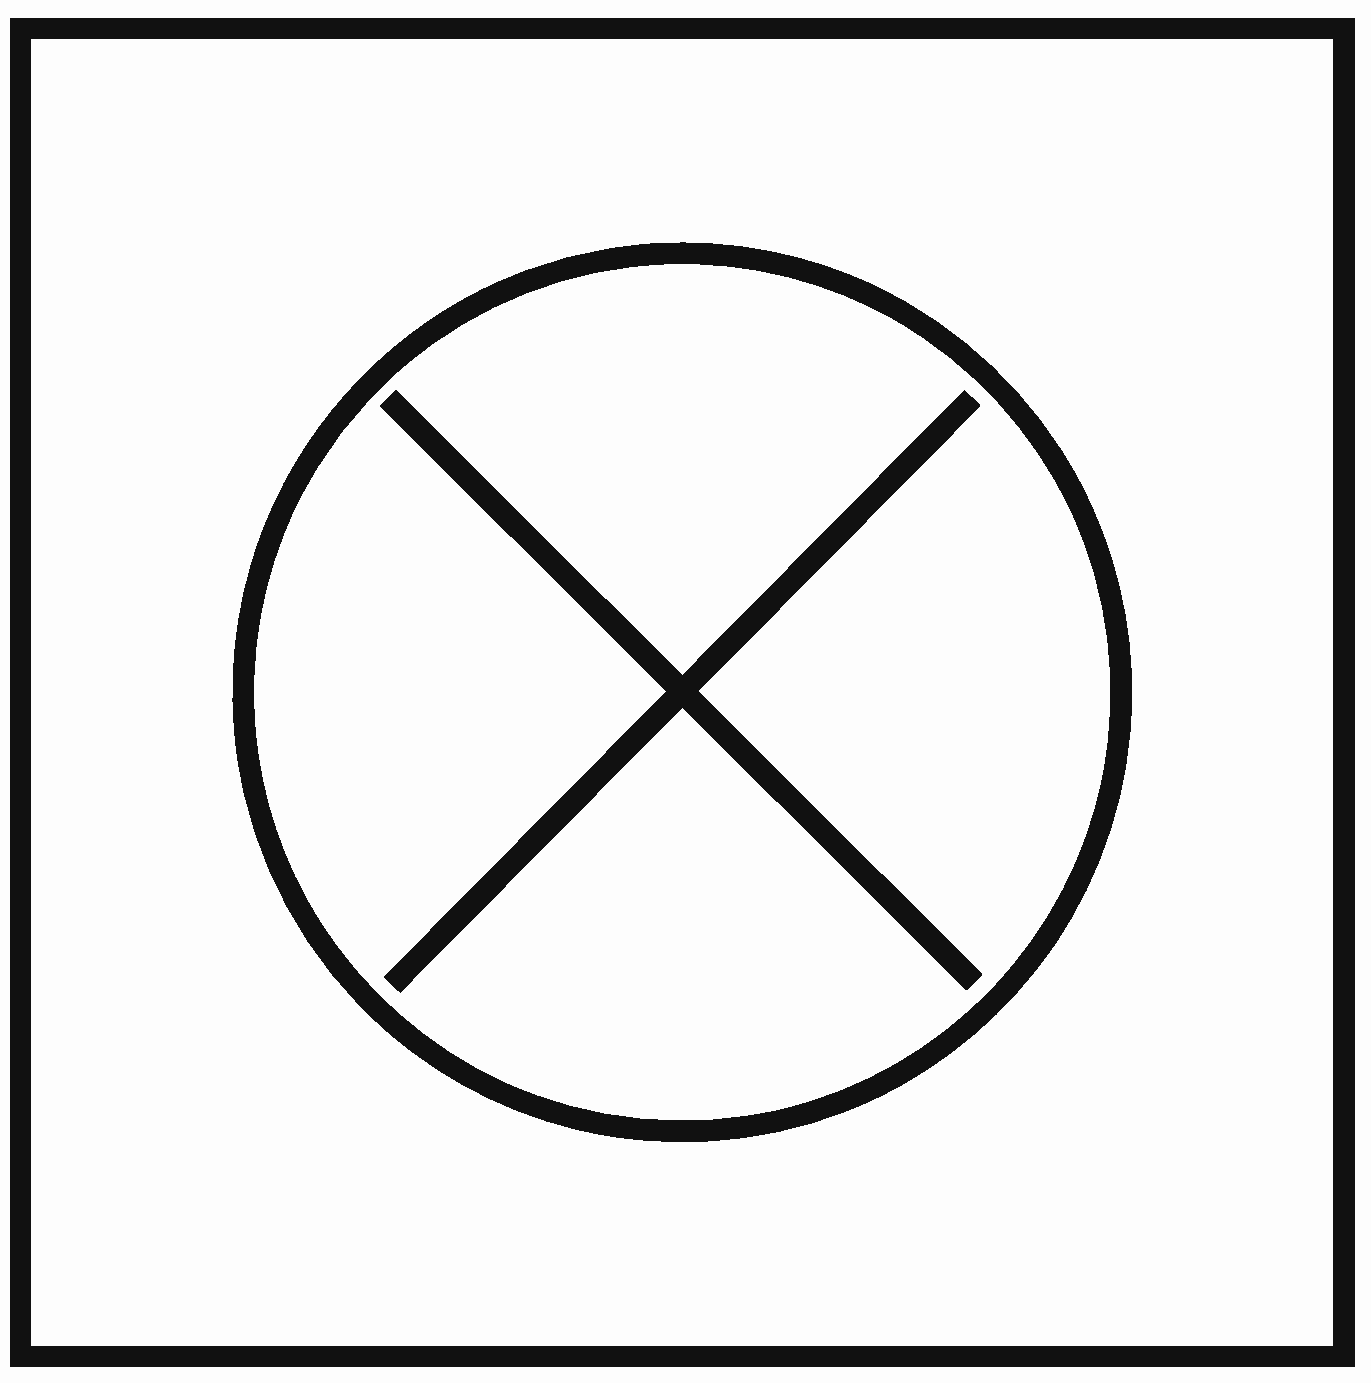
\includegraphics[width=0.3\textwidth]{img/base.pdf}
    \caption{Design of the platform in which the quadrotor must land on}
    \label{fig:finalplatform}
\end{figure}



%\chapter{MBZIRC challenge}\label{chap:thechallenge}
The Mohamed Bin Zayed International Robotics Challenge (MBZIRC) is an international robotics competition, held every two years \cite{challenge_description}. MBZIRC provides an ambitious and technologically demanding set of challenges, that aim to inspire the future of robotics through innovative solutions and technological excellence.\\
Robotics is poised to have a transformative impact in a variety of new markets and on various human social aspects. These include robot applications in disaster response, oil and gas, manufacturing, construction and household chores. Enabling technologies for such applications include robots working more autonomously in dynamic, unstructured environments, while collaborating and interacting with other robots and humans. \\
The competition consists in 3 challenges and this thesis consist in developing a framework to complete challenge number 1 that requires an UAV to land on a moving ground vehicle. 
The specifications of the challenge are:
\begin{itemize}
\item Duration: 20 minutes.
\item UAV initial condition: the participating team positions the UAV in stationary mode on the ground at the start location.
\item UGV initial condition: the ground vehicle is driven into the arena and placed at a random location on the track.
\end{itemize}

 

\subsection{The Arena}
The challenge will be performed in an arena with the following specifications (see figure \ref{fig:arenachallenge}):
\begin{itemize}
\item Outdoor open arena with GPS access.
\item Dimension: approximate  $100m \times 60m$.
\item Track: width 3m, in the shape of a figure 8 (of infinity shape), with boundary marked with white paint.
\item Terrain: relatively smooth and relatively level. 
\item UAV initial start location: 10m away from the arena.
\end{itemize}

\begin{figure}[!htbp]
    \centering
    \includegraphics[width=1.1\textwidth]{img/arena.png}
    \caption{Arena of the challenge}
    \label{fig:arenachallenge}
\end{figure}

\subsection{Landing platform}
The landing platform is mounted on a ground vehicle of approximate dimensions $2.5m \times 1.5m \times 1.5m$ (length, width, height). The moving car starts at a constant speed of $15km/h$, it reduces the speed to $10km/h$ after 6 minutes and to $5 Km/h$ after 12 minutes.\\
The landing platform will be made of a ferrous surface to enable docking using magnetic or suction or other means.
It will be a square of dimensions $1.5m \times 1.5m$, and approximately $1.5m$ above ground, positioned on the vehicle. 
The landing zone inside the landing area is a circle of diameter $1m$. The center of the circle is indicated by an X. The landing area, the landing zone and the marker X are shown in Figure \ref{fig:finalplatform}.
A successful landing is when a point of contact of the UAV is within the landing circle, with propulsion off and rotors not spinning.

\begin{figure}[!htbp]
    \centering
    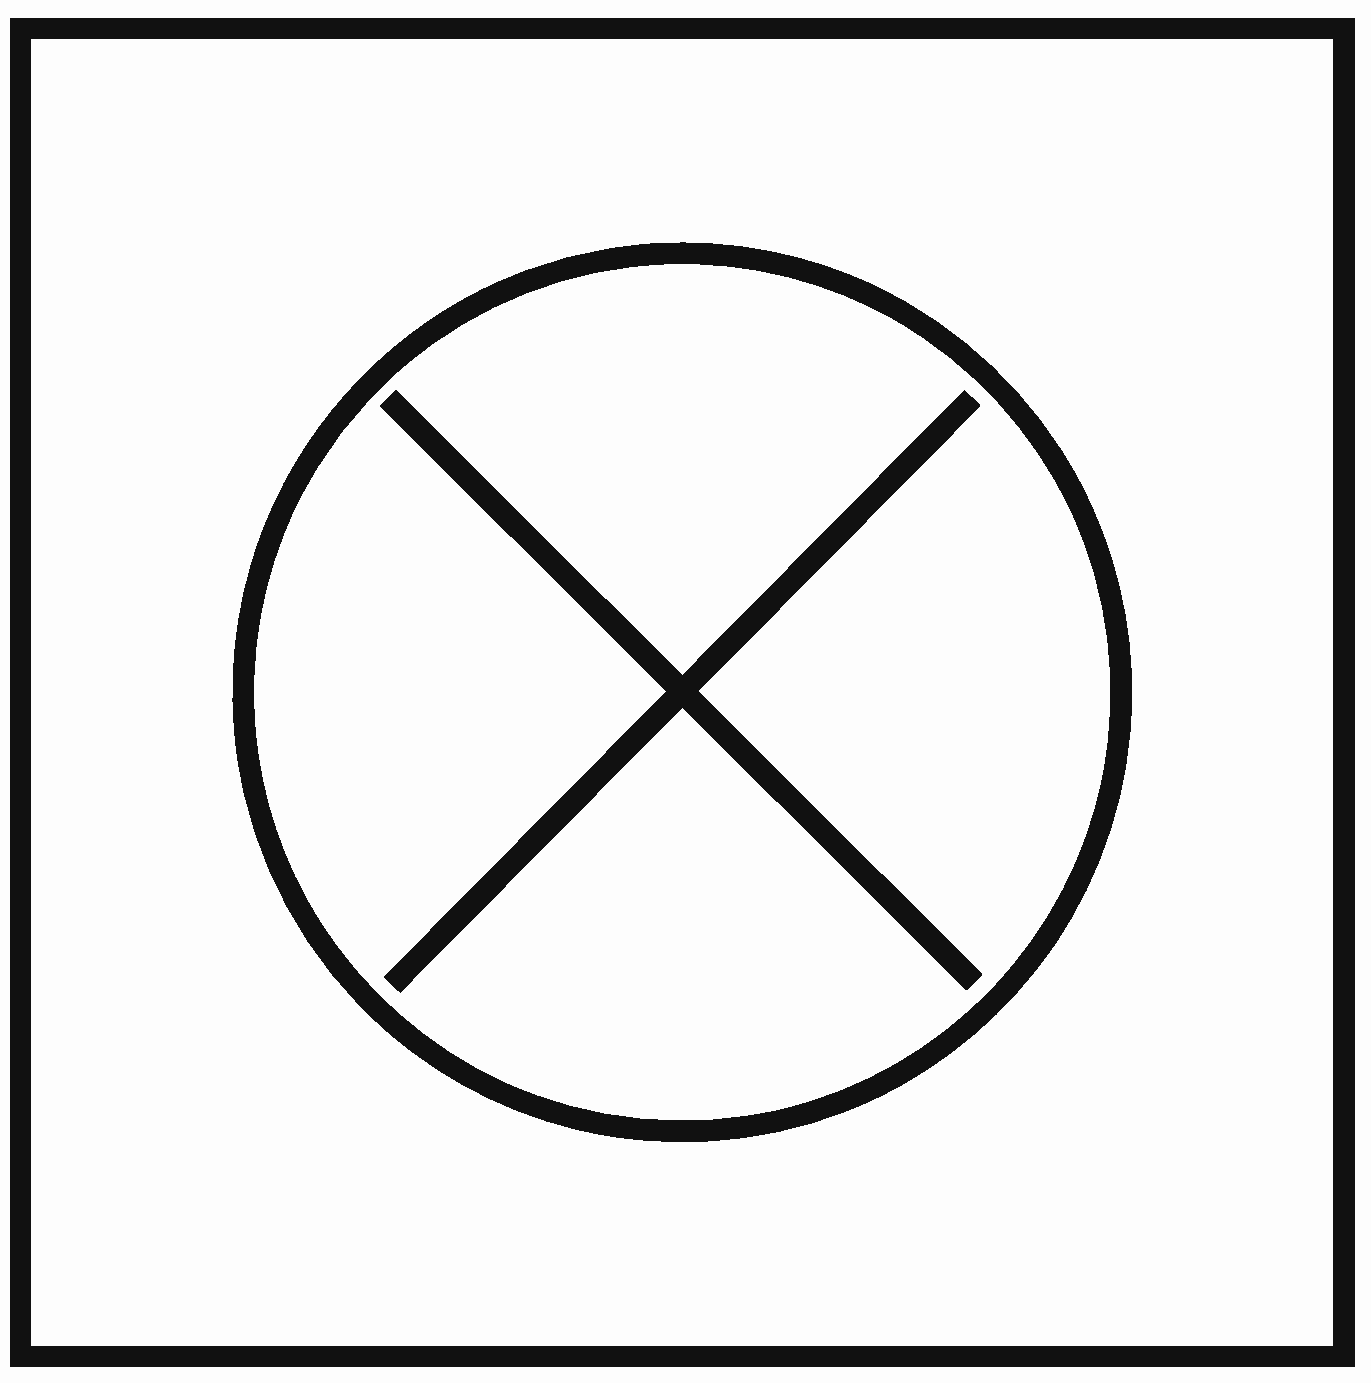
\includegraphics[width=0.5\textwidth]{img/base.pdf}
    \caption{Design of the platform in which the quadrotor must land on}
    \label{fig:finalplatform}
\end{figure}

\subsection{Infinity shape path}
The moving platform will move in an infinity-shape path described in the figure \ref{fig:arenachallenge}. 
We need to describe in a mathematical way this shape in order to use this information when we are estimating the state of the platform and to understand the right moment to perform the landing maneuver.\\
From the specification of the challenge:
\begin{itemize}
\item the car is moving with constant velocity $v_{tan}$ along the path
\item the radius of the circumferences that forms the trajectory is $r_{8}$m
\item the path is making a cross in the middle that creates 4 angles of $\frac{\pi}{2}$ 
\end{itemize}
The easiest way to describe this path is to define how the angle $\theta$ is changing in function of the space. \\
It easy to see that the shape can be seen as a combination of a cross and two circles.
The cross is simply defined as the union between the two line:
\begin{align}
\begin{split}
y &= x \\
y &= -x
\end{split}
\end{align}
while the two circles 
\begin{align}
\begin{split}
y^2 + (x - x_0)^2 &= r_{8}^2 \\
y^2 + (x + x_0)^2 &= r_{8}^2 
\end{split}
\end{align}
It easy to see that if we want the intersections between these two functions to be exactly in the 4 points we have to choose 
\begin{align}
\begin{split}
x_0 = \frac{\sqrt{2}}{2}r_{8}
\end{split}
\end{align}
That correspond to the 4 intersections coordinate
\begin{align}
\begin{split}
\Big(\frac{\sqrt{2}}{2}r_{8},\frac{\sqrt{2}}{2}r_{8}\Big);
\Big(\frac{\sqrt{2}}{2}r_{8},-\frac{\sqrt{2}}{2}r_{8}\Big);
\Big(-\frac{\sqrt{2}}{2}r_{8},-\frac{\sqrt{2}}{2}r_{8}\Big);
\Big(-\frac{\sqrt{2}}{2}r_{8},\frac{\sqrt{2}}{2}r_{8}\Big)
\end{split}
\end{align}

\begin{figure}[!htbp]
  \centering
 {\includegraphics[width=0.48\textwidth]{img/constructionshape1_.png}\label{fig:constuctinfinity1}}
  \hfill
  {\includegraphics[width=0.48\textwidth]{img/constructionshape2_.png}\label{fig:constuctinfinity2}}
  \caption{How to construct the infinity-shape path}
\end{figure}

If we travel over the two circumferences the intersections correspond to angles $\theta = \pm \frac{3\pi}{4}$. \\
Now it is obvious to see that the path is symmetric and it can be divided in 4 parts and describing how the angle is changing in one of this section, the whole trajectory is defined.\\
We can observe that:
\begin{align}
\theta(x) =
\begin{cases}
    -\frac{x}{r_{8}}  &x\in \Big[0,\frac{3\pi}{4}r_{8}\Big] \quad \quad \ \ \  \\[10pt]
    -\frac{3\pi}{4} &x\in \Big[\frac{3\pi}{4}r_{8} ,\frac{3\pi}{4}r_{8} + r_{8}\Big]
\end{cases}
\end{align}
This function define a quarter of the trajectory \ref{fig:quarter_path} in function of the radius $r_{8}$ of the path.\\
It is now possible to use it to generate the entire trajectory $( x(t) , y(t) )$ \ref{fig:entire_path}: \\ we know that the length of the path is $$l = 4(\frac{3\pi}{4}r_{8} + r_{8})$$
and given the constant velocity $v_{tan}$ we can calculate the time to complete the trajectory 
$$T = \frac{l}{v_{tan}}$$
and it is simple to define $\theta(t)$ just stretching or shrinking $\theta(x)$ .\\
So we can now define:
\begin{align}
\begin{split}
\dot{x} &= v_{tan} cos(\theta(t)) \\
\dot{y} &= v_{tan} sin(\theta(t))
\end{split}
\end{align}
And finally we also need the discretized verison obtain just by forward Euler approximation:
\begin{align}
\begin{split}
x_k &= x_{k-1} + dt \big(v_{tan k-1} cos(\theta_{k-1})\big) \\
y_k &= y_{k-1} + dt \big(v_{tan k-1} sin(\theta_{k-1})\big)
\end{split}
\end{align}

\begin{figure}[!htbp]
  \centering
 {\includegraphics[width=0.8\textwidth]{img/angle_x.eps}\label{fig:quarter_theta}}
  \hfill
  {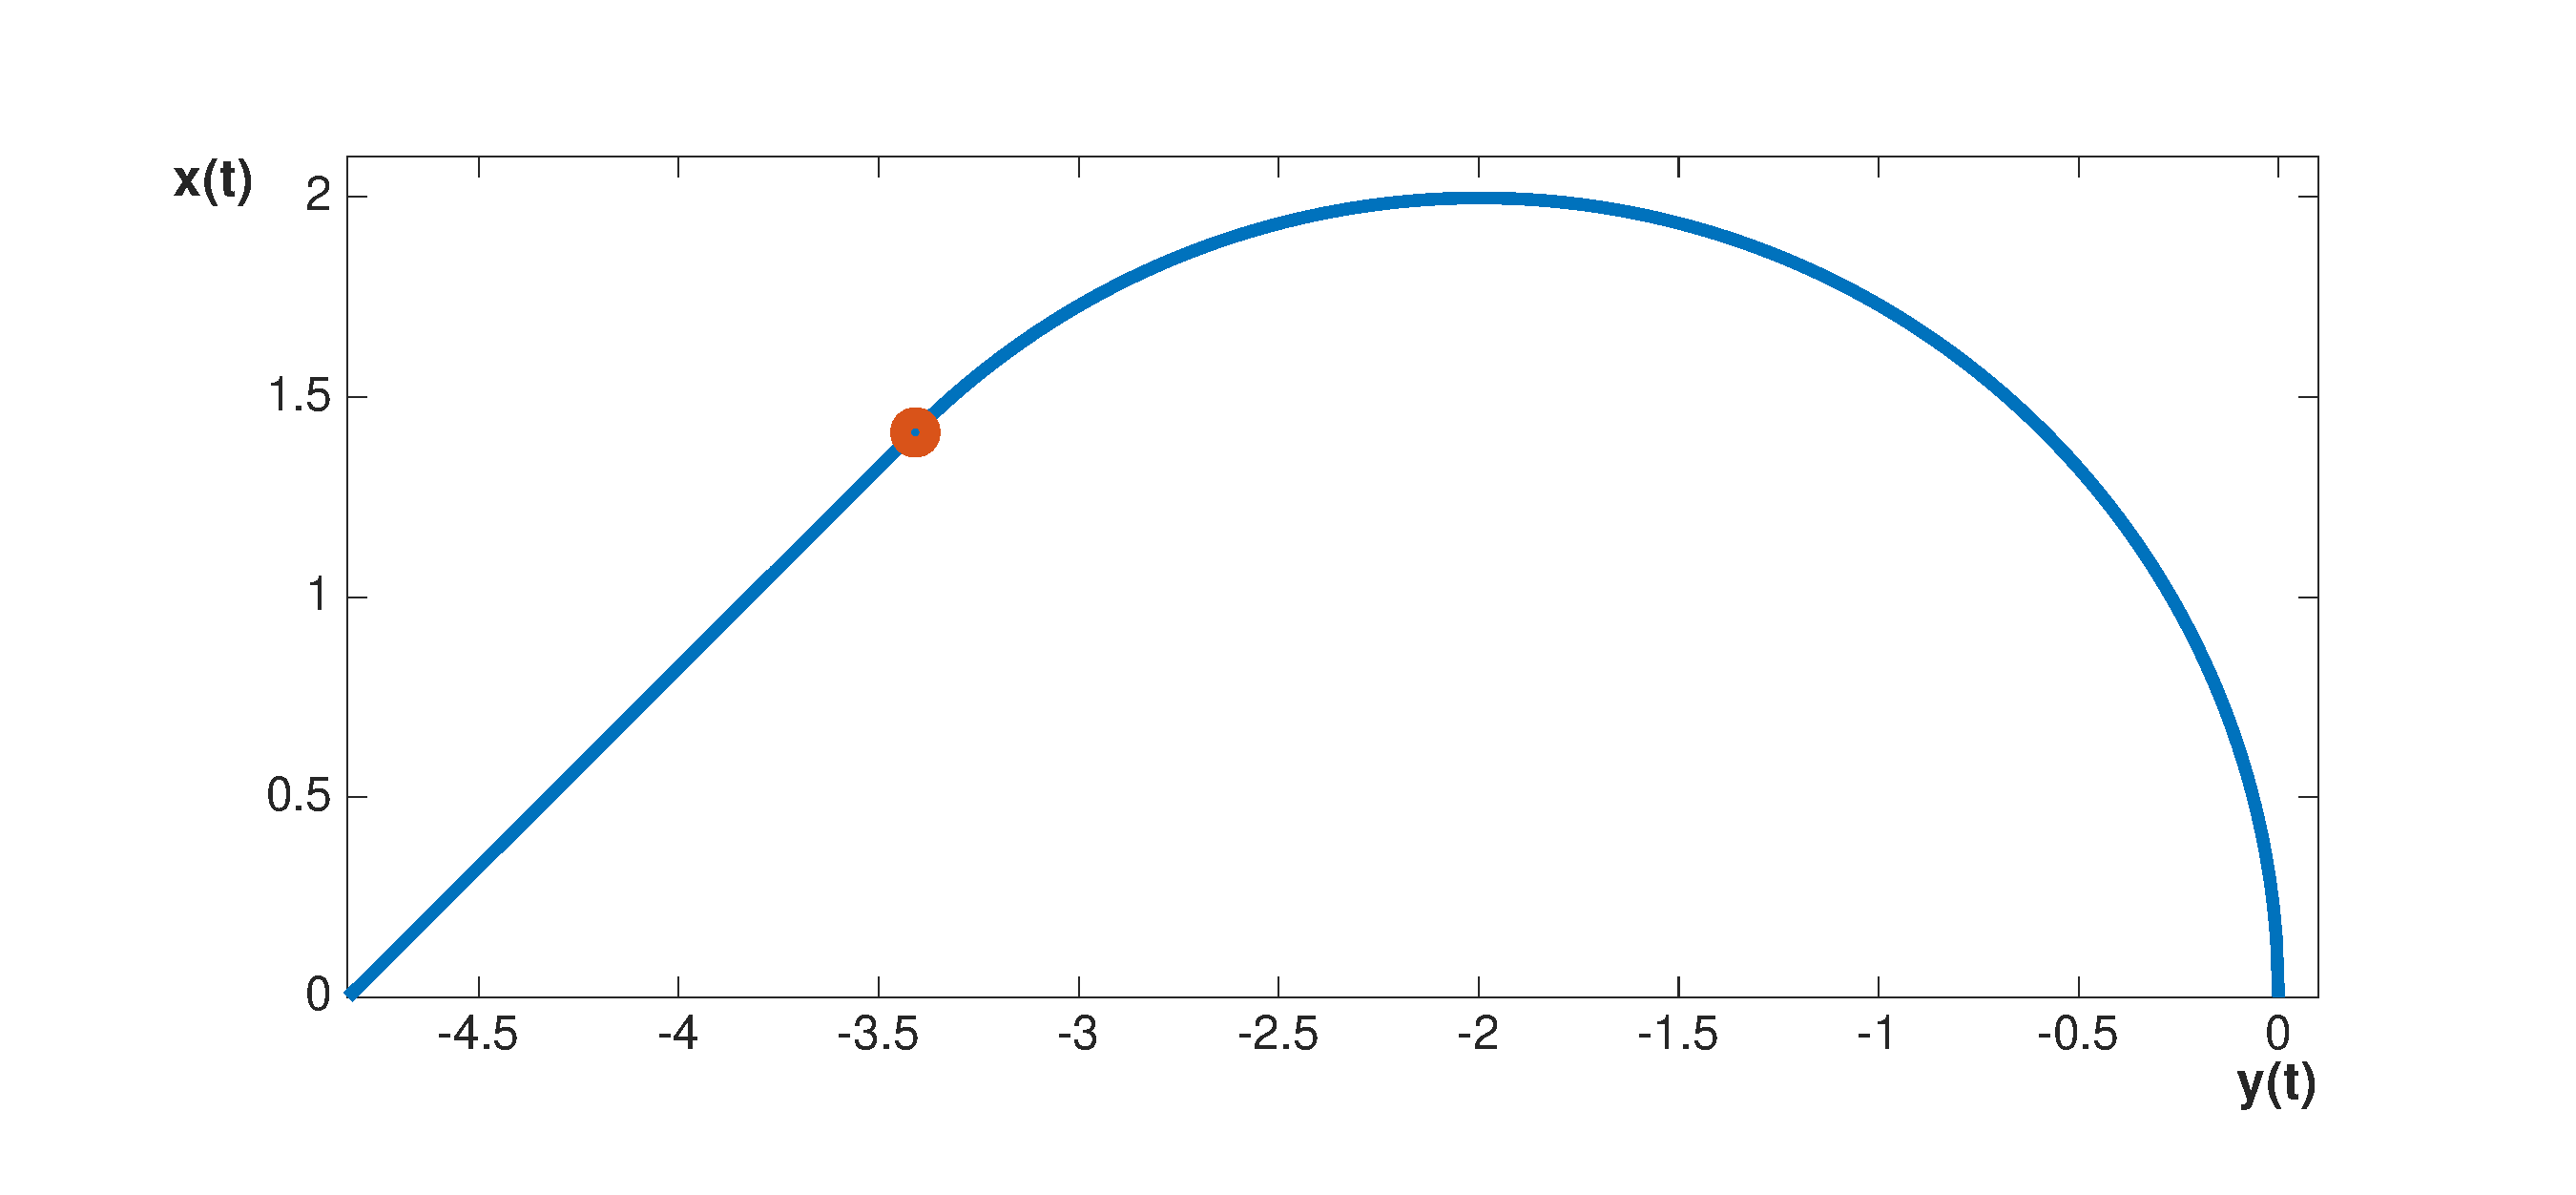
\includegraphics[width=0.8\textwidth]{img/path_x_quarter.eps}\label{fig:quarter_xy}}
  \caption{The parametrization of a quarter of the path}
  \label{fig:quarter_path}
\end{figure}

\begin{figure}[!htbp]
    \centering
    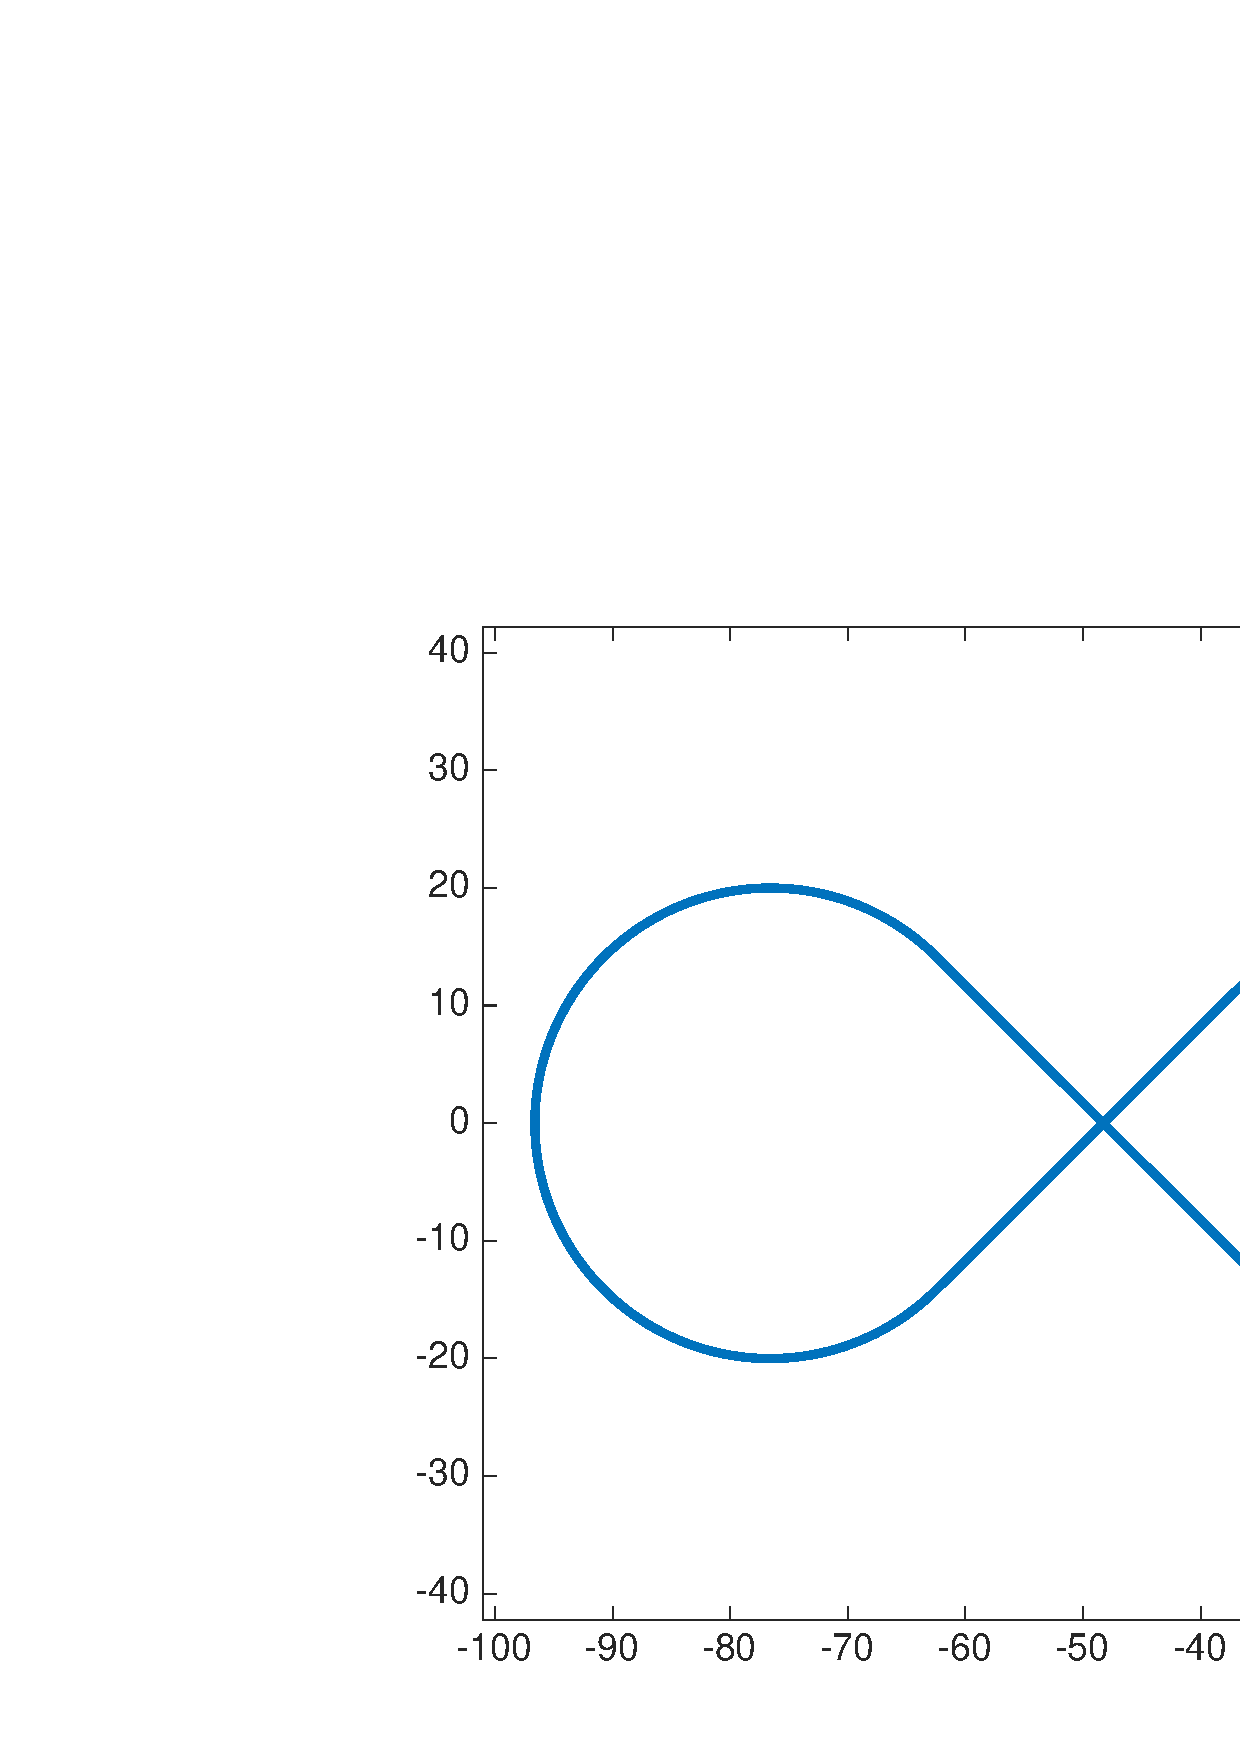
\includegraphics[width=1\textwidth]{img/infinityshapepath.png}
    \caption{Infinity-shape path}
    \label{fig:entire_path}
\end{figure}

\section{Simulation}


\chapter{General Framework}\label{chap:general_framework}

\begin{figure}[!ht]
    \centering
    \includegraphics[width=0.97\textwidth]{img/pipeline_diagram.png}
    \caption{Pipeline}
    \label{fig:pipeline_diagram}
\end{figure}

\subsection{SVO \& MSF}
are calculating the best estimation of the state of quadrotor based on data from a camera and an IMU
\subsubsection{SVO front looking camera}
explanation about base in fov\\
Fish eye or not fish eye? pros and cons
\subsection{Base Detection \& Base Tracking}
given images taken from a camera on the quadrotor, it is searching the landing platform and estimating its state
\subsection{Area Exploration \& Trajectory Generation}
considering the state of the quadrotor and of the landing platform, they are calculating where the quadrotor must go and with which trajectory. 

\subsection{Flight Control \& Copilot}
given the desired trajectory, they are computing the controls that must be applied to the quad in order to follow such trajectory

\chapter{Base detection and tracking}\label{chap:base_tracking}
One part of the work is focused on the estimation of the state of the moving platform. This is necessary in order to have a good prediction of the final state that the quadrotor must have in order to proper land on the moving car. \\ With the method described in this section, every time we detect the platform we can estimate its position, orientation and velocity vector in world coordinate frame, so we can predict where the platform will be in $t$ seconds and where the quadrotor should go to successfully complete the mission.\\ 


An EKF  \cite{kalmanfilter} is design in order to have the most reliable value of the state of the platform.\\
Kalman filtering is an algorithm that uses a series of noisy measurements observed over time and produces estimates of unknown variables that tend to be more precise than those based on a single measurement alone, by using Bayesian inference and estimating a joint probability distribution over the variables for each time frame.\\
The algorithm works in a two-step process:
\begin{itemize}
\item In the prediction step, the Kalman filter produces estimates of the current state variables, along with their uncertainties, based on a model of the system:
\begin{align}
\boldsymbol{x}_k = f(\boldsymbol{x}_{k-1},\boldsymbol{u}_k) + \boldsymbol{w}_k
 \label{eq:ekf1}
\end{align}
\item Once the outcome of the next measurement is observed:
\begin{align}
\boldsymbol{z}_k = h(\boldsymbol{x}_{k}) + \boldsymbol{v}_k
 \label{eq:ekf2}
\end{align}
these estimates are updated using a weighted average, with more weight being given to estimates with higher certainty.
\end{itemize}
In the extended Kalman filter, the state transition and observation models don't need to be linear functions of the state but may instead be differentiable functions.\\
($\boldsymbol{w}_k$ and $\boldsymbol{v}_k$ are the process and observation noises which are both assumed to be zero mean multivariate Gaussian noises with covariance $\boldsymbol{Q}_k$ and $\boldsymbol{R}_k$ respectively. $\boldsymbol{u}_k$ is the control vector).

The algorithm is recursive. It can run in real time, using only the present input measurements and the previously calculated state and its uncertainty matrix; no additional past information is required.\\
The Kalman filter does not require any assumption that the errors are Gaussian. However, the filter yields the exact conditional probability estimate in the special case that all errors are Gaussian-distributed.\\
Initialization
\begin{align}
\begin{split}
\boldsymbol{x}_{0|0} = x_0\\
\boldsymbol{P}_{0|0} = P_0
\end{split}
\end{align}
In this case the prediction equations are continuous in time, so for the prediction step of the EKF we have to solve:
\begin{align}
\begin{split}
\boldsymbol{\dot{\hat{x}}}(t) &= f(\boldsymbol{\hat{x}}(t),\boldsymbol{u}(t)) \\
\boldsymbol{\dot{P}}(t) &= \boldsymbol{F}(t) \boldsymbol{P}(t) + \boldsymbol{P}(t)\boldsymbol{F}(t)^{\top } + \boldsymbol{Q}(t)
\end{split}
\end{align}
for $t \in (t_{k-1}, t_k)$ where
\begin{align}
\begin{split}
\boldsymbol{\hat{x}}(t_{k-1}) &= \hat{x}_{k-1|k-1} \\
\boldsymbol{P}(t_{k-1}) &= P_{k-1|k-1}
\\
{\boldsymbol{F}}(t)&=\left.{\frac  {\partial f}{\partial {\boldsymbol{x}}}}\right\vert _{{{\hat  {{\boldsymbol{x}}}}(t),{\boldsymbol{u}}(t)}}  \\
\boldsymbol{\hat{x}}_{k|k-1} &= \boldsymbol{\hat{x}}(t_{k}) \\
\boldsymbol{P}_{k|k-1} &= \boldsymbol{P}(t_{k})
\end{split}
\end{align}
In order to save some computation we can discretize the dynamicin order to have shorter computation during the prediction step of the EKF:
\begin{align}
\begin{split}
\boldsymbol{\hat{x}}_{k|k-1} &= f(\boldsymbol{\hat{x}}_{k-1|k-1},\boldsymbol{u}_k) \\
\boldsymbol{P}_{k|k-1} &= \boldsymbol{F}_{k-1} \boldsymbol{P}_{k-1|k-1}\boldsymbol{F}_{k-1}^{\top } + \boldsymbol{Q}_{k}
\end{split}
\end{align}
where the state transition matrix is defined to be the following Jacobians:
\begin{align}
\begin{split}
\boldsymbol{F}_{k-1}&= \left.{\frac{\partial f}{\partial {\boldsymbol{x}}}} \right \vert_{\hat{\boldsymbol{x}}_{k-1|k-1},\boldsymbol{u}_{k}} 
\end{split}
\end{align}
While the update equations are discrete in time and they yield to the following update step: 
\begin{align}
\begin{split}
\boldsymbol{K}_{k} &= \boldsymbol{P}_{k|k-1} \boldsymbol{H}_{k}^{\top }(\boldsymbol{H}_{k} \boldsymbol{P}_{k|k-1} \boldsymbol{H}_{k}^{\top }+ \boldsymbol{R}_{k})^{-1}
\\
\hat{\boldsymbol{x}}_{k|k} &= \hat{\boldsymbol{x}}_{k|k-1} + \boldsymbol{K}_{k} (\boldsymbol{z}_{k}-h(\hat{\boldsymbol{x}}_{k|k-1}))
\\
\boldsymbol{P}_{k|k} &=(\boldsymbol{I}-\boldsymbol{K}_{k}\boldsymbol{H}_{k})\boldsymbol{P}_{k|k-1}
\end{split}
\end{align}
where the observation matrix is defined to be the following Jacobian:

\begin{align}
\begin{split}
\boldsymbol{H}_{k} = \left.{\frac{\partial h}{\partial {\boldsymbol{x}}}} \right \vert_{\hat{\boldsymbol{x}}_{k|k-1}}
\end{split}
\end{align}

\section{Prediction update: non-holonomic model}
The platform is considered as a car and simulated with a non-holonomic model \ref{fig:nonholonomicmodel}. 
\begin{figure}[!ht]
    \centering
    \includegraphics[width=0.5\textwidth]{img/non_holonomic_model.png}
    \caption{Non-holonomic model}
    \label{fig:nonholonomicmodel}
\end{figure}

In this model the state is defined as $\boldsymbol{x} = (x, y, z,\theta , v, \phi)$:
It corresponds to the 3 position in a space $(x,y,z)$ and the yaw angle of the platform $(\theta)$ w.r.t. the world frame, the forward velocity ($v$) and the angle of the front wheels ($\phi$). The system depends on a parameter $L$ that corresponds to the distance between the front and the back wheels.\\
In this model the control input are the change in velocity $v$ and in the angle of curvature $\phi$. \\
The equation of motion in continuous time are:
\begin{align}
\boldsymbol{\dot{x}} = f(\boldsymbol{x},\boldsymbol{u}) \nonumber
\end{align}
\begin{align}
\boldsymbol{\dot{x}} = 
\begin{bmatrix}
\dot{x}  \\[10pt]
\dot{y}  \\[10pt]
\dot{z} \\[10pt]
\dot{\theta} \\[10pt]
\dot{v}  \\[10pt]
\dot{\phi}
\end{bmatrix}
= 
\begin{bmatrix}
v cos(\theta) \\[10pt]
v sin(\theta) \\[10pt]
 0 \\[10pt]
\frac{v}{L}tan(\phi)\\[10pt]
u_1 \\[10pt]
 u_2 
\end{bmatrix}
\label{eq:equation_nonholonomic_continuos}
\end{align}
It is possible to discretize these dynamics in $t \in (t_{k-1}, t_k)$ with a first order finite difference:
\begin{align}
\boldsymbol{\dot{x}} \approx \frac{\boldsymbol{x}_k - \boldsymbol{x}_{k-1} }{dt} \approx f(\boldsymbol{x}_{k-1},\boldsymbol{u}_k) \nonumber
\end{align}
with $\boldsymbol{x}_k = \boldsymbol{x}(t_k)$, $\boldsymbol{x}_{k-1} = \boldsymbol{x}(t_{k-1})$, $dt = t_k - t_{k-1}$
\begin{align}
\boldsymbol{x_k} = 
\begin{bmatrix}
x_k  \\[10pt]
y_k  \\[10pt]
z_k \\[10pt]
\theta_k \\[10pt]
v_k  \\[10pt]
\phi_k
\end{bmatrix}
= 
\begin{bmatrix}
 x_{k-1} + dt \big(v_{k-1} cos(\theta_{k-1})\big) \\[10pt]
 y_{k-1} + dt \big(v_{k-1} sin(\theta_{k-1})\big) \\[10pt]
 z_{k-1} \\[10pt]
 \theta_{k-1} + dt\Big(\frac{v_{k-1}}{L}tan(\phi_{k-1}) \Big)\\[10pt]
v_{k-1} + dt \big(u_{1k}\big) \\[10pt]
\phi_{k-1} + dt \big(u_{2k}\big) 
\end{bmatrix}
\label{eq:equation_nonholonomic_discrete}
\end{align}

In order to solve the former system, we have anyway to find a numerical solution. For this purpose we use a    
Runge-Kutta scheme  \cite{wiki_runge_kutta}.\\
In numerical analysis, the Runge-Kutta methods are a family of implicit and explicit iterative methods used in temporal discretization for the approximate solutions of ordinary differential equations.\\
The most widely known member of the Runge-Kutta family is generally referred to as RK4.\\
Let an initial value problem be specified as follows:
\begin{align}
\begin{split}
{\dot {y}}&=f(t,y) \\
y(t_{0})&=y_{0}
\end{split}
\end{align}
$y$ is an unknown function (scalar or vector) of time $t$, which we would like to approximate and the function $f$ and the data $t_{0}$, $y_{0}$ are given.\\
Now pick a step-size $h > 0$ and define
\begin{align}
\begin{split}
y_{k+1}&=y_{k}+{\tfrac {h}{6}}\left(\alpha_{1}+2\alpha_{2}+2\alpha_{3}+\alpha_{4}\right),\\
t_{k+1}&=t_{k}+h
\end{split}
\end{align}
for $k = 0, 1, 2, 3, ...,$ using
\begin{align}
\begin{split}
\alpha_{1}&=f(t_{k},y_{k}),\\
\alpha_{2}&=f(t_{k}+{\frac {h}{2}},y_{k}+{\frac {h}{2}}\alpha_{1}),\\
\alpha_{3}&=f(t_{k}+{\frac {h}{2}},y_{k}+{\frac {h}{2}}\alpha_{2}),\\
\alpha_{4}&=f(t_{k}+h,y_{k}+h\alpha_{3}).
\end{split}
\end{align}
Here  $y_{k+1}$ is the RK4 approximation of $y(t_{k+1})$, and it is determined by the present value ($y_{k}$) plus the weighted average of four increments.

\subsection{Straight and circular path} \ref{subsec:circularlinearmodel}
We assume the input $u_1$ and $u_2$  are equal to zero. In this way we can have three type of movement:
\begin{itemize}
\item the platform can be static ($v_f(0) = 0$)
\item it can move in a straight line ($v_f(0) \neq 0$ and $\phi(0) = 0$)
\item it can move in a circle ($v_f(0) \neq 0$ and $\phi(0) \neq 0$)
\end{itemize}

\subsection{Infinity shape path}
As described in charapter \label{chap:thechallenge}, the moving platform will move in an infinity-shape path described in the figure \ref{fig:arenachallenge}. \\
We need to describe in a mathematical way this shape in order to use this information when we are estimating the state of the platform and to understand the right moment to perform the landing maneuver.\\
From the specification of the challenge:
\begin{itemize}
\item the car is moving with constant velocity $v_{tan}$ along the path
\item the radius of the circumferences that forms the trajectory is $r_{8}$m
\item the path is making a cross in the middle that creates 4 angles of $\frac{\pi}{2}$ 
\end{itemize}
The easiest way to describe this path is to define how the angle $\theta$ is changing in function of the space. \\
It easy to see that the shape can be seen as a combination of a cross and two circles.
The cross is simply defined as the union between the two line:
\begin{align}
\begin{split}
y &= x \\
y &= -x
\end{split}
\end{align}
while the two circles 
\begin{align}
\begin{split}
y^2 + (x - x_0)^2 &= r_{8}^2 \\
y^2 + (x + x_0)^2 &= r_{8}^2 
\end{split}
\end{align}
It easy to see that if we want the intersections between these two functions to be exactly in the 4 points we have to choose 
\begin{align}
\begin{split}
x_0 = \frac{\sqrt{2}}{2}r_{8}
\end{split}
\end{align}
That correspond to the 4 intersections coordinate
\begin{align}
\begin{split}
\Big(\frac{\sqrt{2}}{2}r_{8},\frac{\sqrt{2}}{2}r_{8}\Big);
\Big(\frac{\sqrt{2}}{2}r_{8},-\frac{\sqrt{2}}{2}r_{8}\Big);
\Big(-\frac{\sqrt{2}}{2}r_{8},-\frac{\sqrt{2}}{2}r_{8}\Big);
\Big(-\frac{\sqrt{2}}{2}r_{8},\frac{\sqrt{2}}{2}r_{8}\Big)
\end{split}
\end{align}

\begin{figure}[!htbp]
  \centering
 {\includegraphics[width=0.4\textwidth]{img/constructionshape1_.png}\label{fig:constuctinfinity1}}
  \hfill
  {\includegraphics[width=0.4\textwidth]{img/constructionshape2_.png}\label{fig:constuctinfinity2}}
  \caption{How to construct the infinity-shape path}
\end{figure}

If we travel over the two circumferences the intersections correspond to angles $\theta = \pm \frac{3\pi}{4}$. \\
Now it is obvious to see that the path is symmetric and it can be divided in 4 parts and describing how the angle is changing in one of this section, the whole trajectory is defined.\\
We can observe that:
\begin{align}
\theta(x) =
\begin{cases}
    -\frac{x}{r_{8}}  &x\in \Big[0,\frac{3\pi}{4}r_{8}\Big] \quad \quad \ \ \  \\[10pt]
    -\frac{3\pi}{4} &x\in \Big[\frac{3\pi}{4}r_{8} ,\frac{3\pi}{4}r_{8} + r_{8}\Big]
\end{cases}
\end{align}
This function define a quarter of the trajectory \ref{fig:quarter_path} in function of the radius $r_{8}$ of the path.\\
It is now possible to use it to generate the entire trajectory $( x(t) , y(t) )$ \ref{fig:entire_path}: \\ we know that the length of the path is $$l = 4(\frac{3\pi}{4}r_{8} + r_{8})$$
and given the constant velocity $v_{tan}$ we can calculate the time to complete the trajectory 
$$T = \frac{l}{v_{tan}}$$
and it is simple to define $\theta(t)$ just stretching or shrinking $\theta(x)$ .\\
So we can now define:
\begin{align}
\begin{split}
\dot{x} &= v_{tan} cos(\theta(t)) \\
\dot{y} &= v_{tan} sin(\theta(t))
\end{split}
\end{align}
And finally we also need the discretized verison obtain just by forward Euler approximation:
\begin{align}
\begin{split}
x_k &= x_{k-1} + dt \big(v_{tan k-1} cos(\theta_{k-1})\big) \\
y_k &= y_{k-1} + dt \big(v_{tan k-1} sin(\theta_{k-1})\big)
\end{split}
\end{align}

\begin{figure}[!htbp]
 \centering
   \begin{subfigure}[b]{0.42\textwidth}
     \includegraphics[width=\textwidth]{img/angle_x.eps}
        \caption{Angle in function of the space}
        \label{fig:quarter_theta}
   \end{subfigure}
   \hfill
   \begin{subfigure}[b]{0.45\textwidth}
     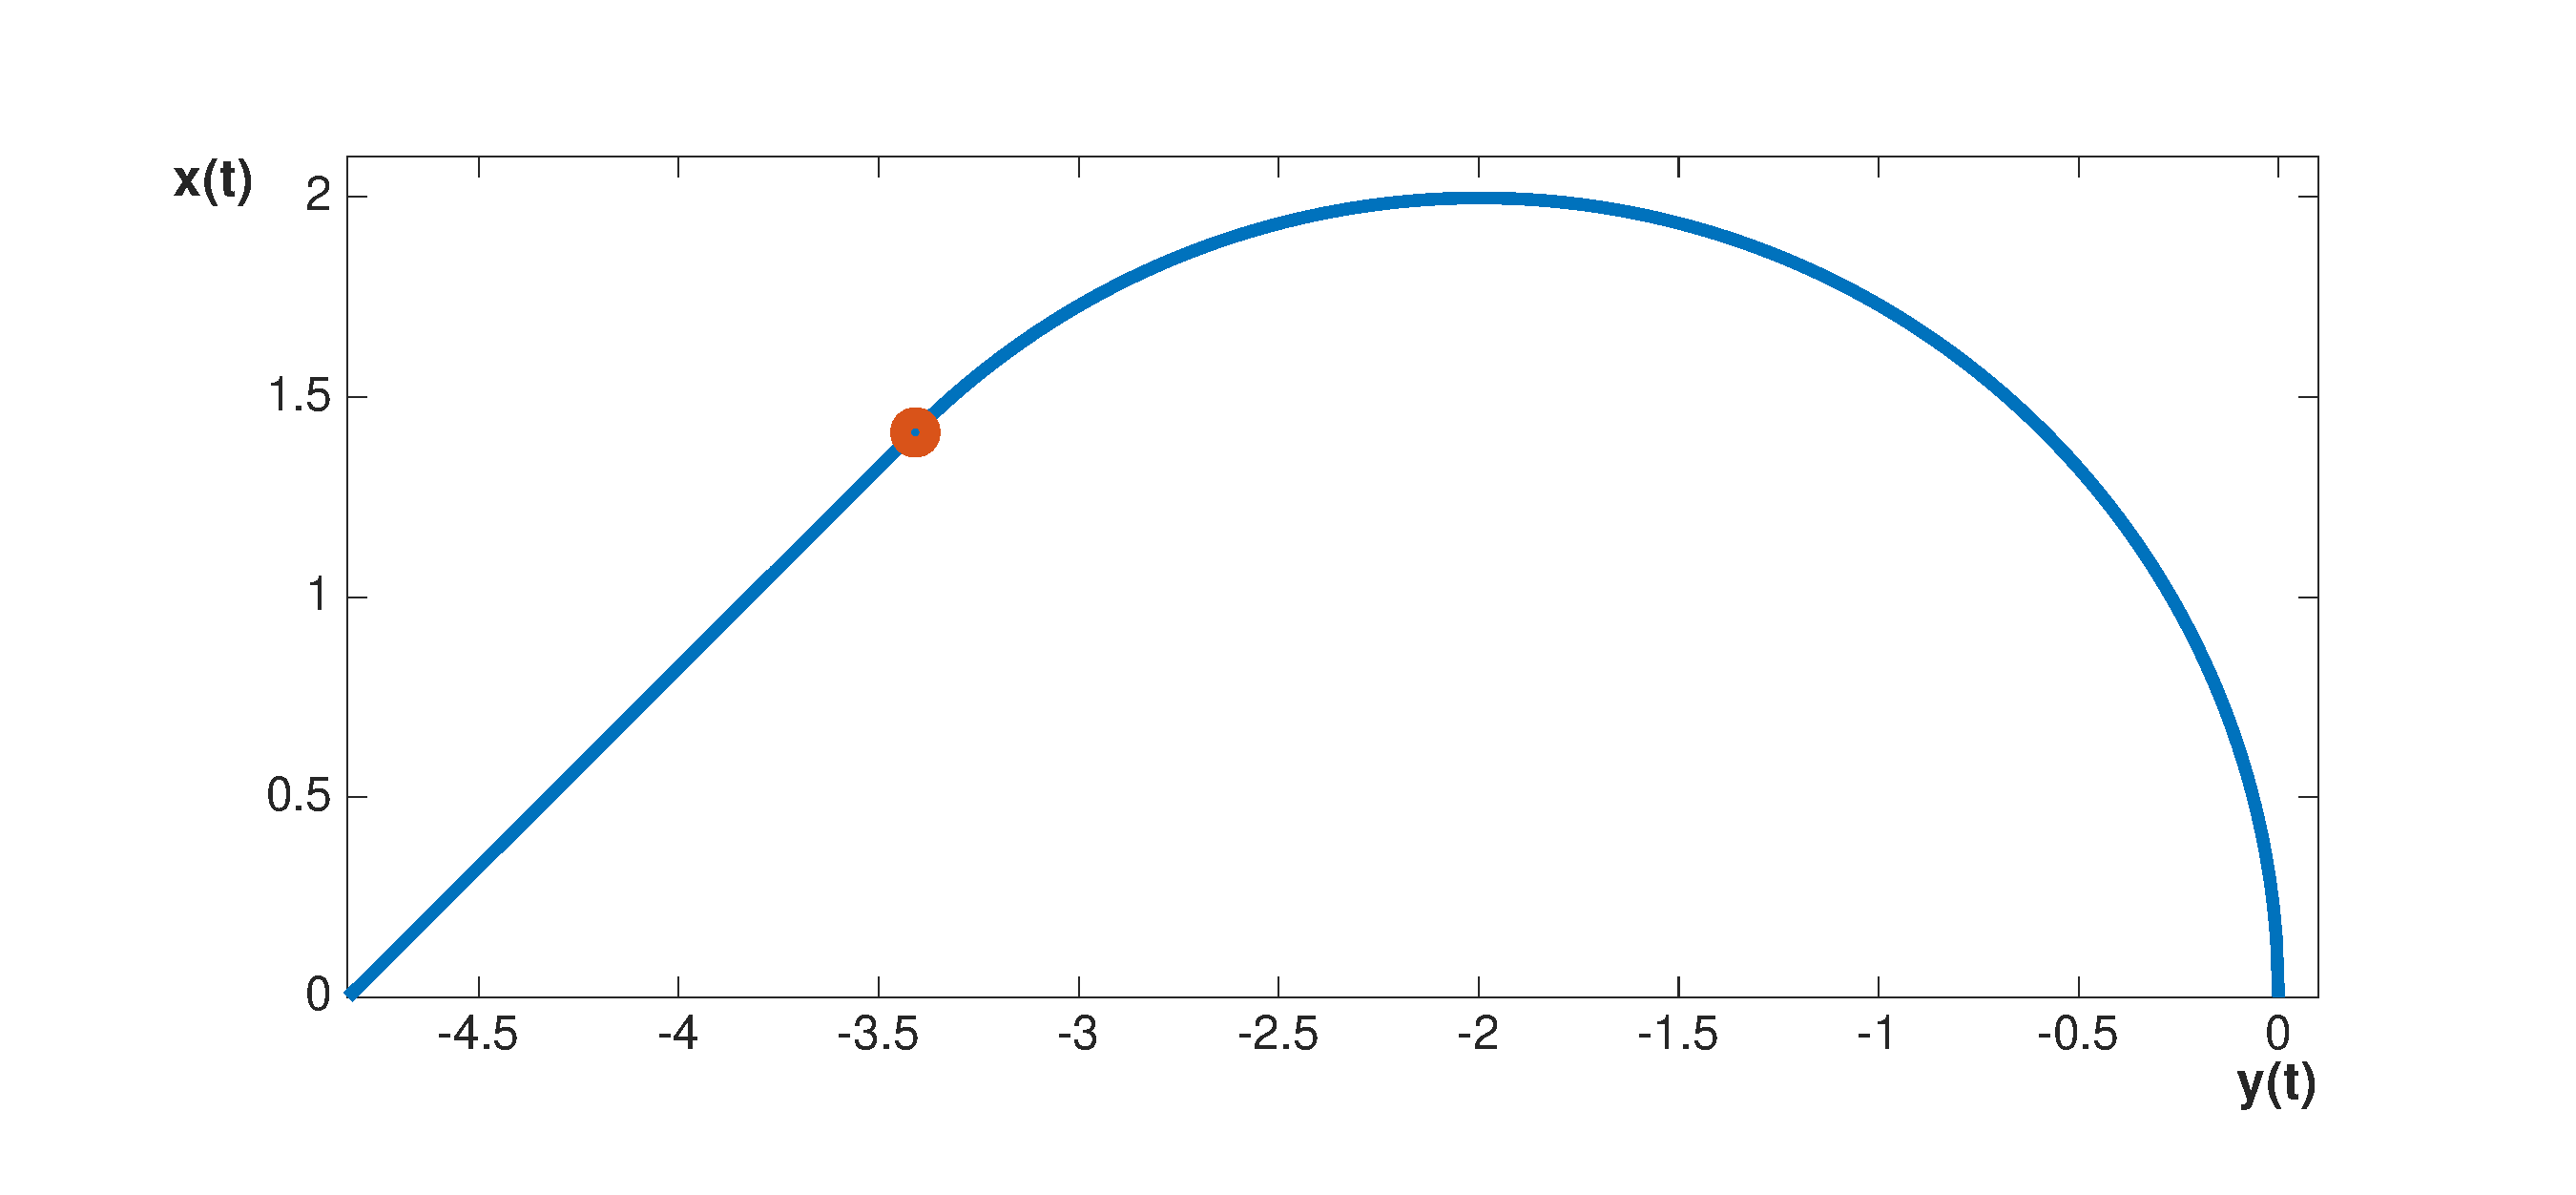
\includegraphics[width=\textwidth]{img/path_x_quarter.eps}
        \caption{One quarter of the path}
       \label{fig:quarter_xy}
   \end{subfigure}
   
   \begin{subfigure}[b]{0.45\textwidth}
     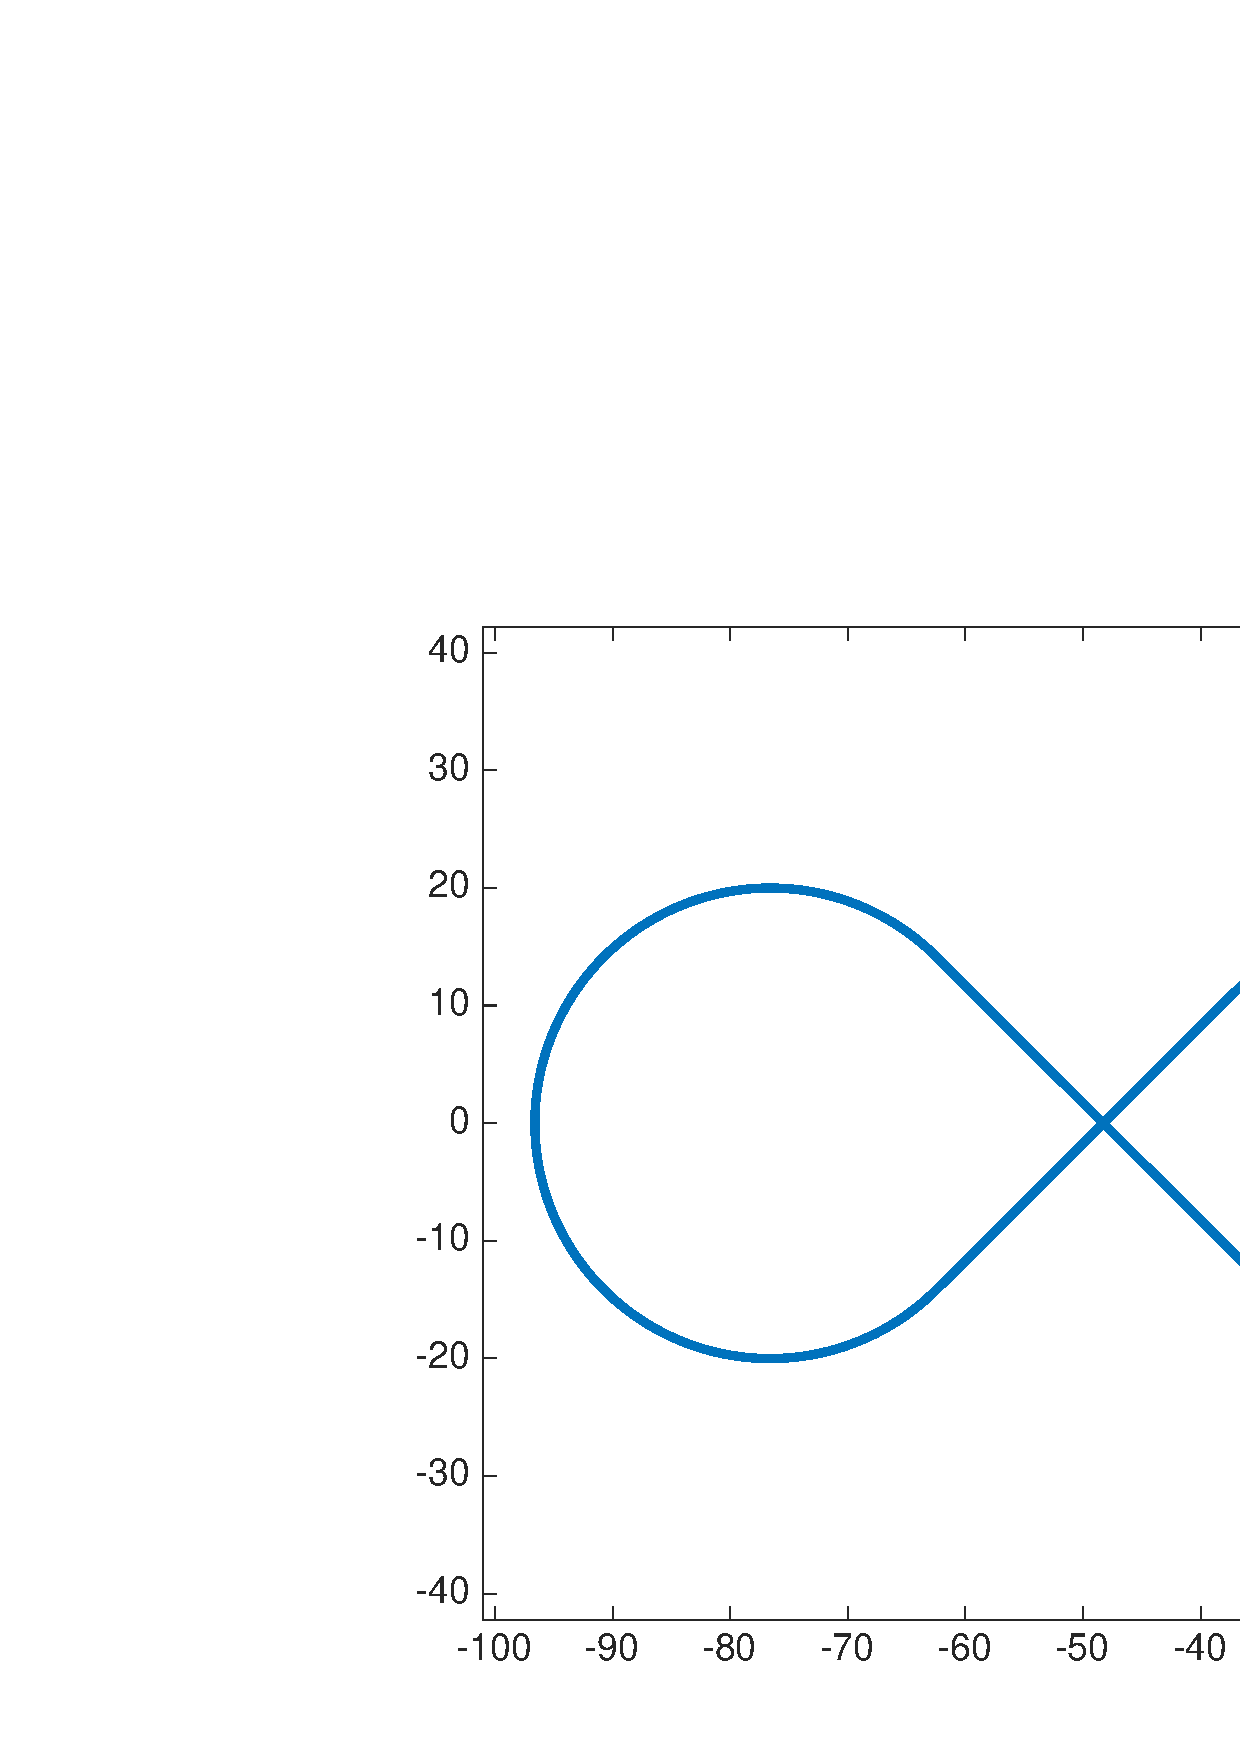
\includegraphics[width=\textwidth]{img/infinityshapepath.png}
       \label{fig:entire_xy}
   \end{subfigure}
    \caption{The parametrization of the path}
  \label{fig:path}
  \end{figure}
  
From these calculations we can conclude that the final trajectory of the platform is only a composition of a linear and a circular movement (for a given determinate amount of time). So the model described in \ref{subsec:circularlinearmodel} can be used also in the final implementation.

\section{Measurement update}
From equation \ref{eq:equation_nonholonomic_discrete} we have the variables that describe the state of the moving car. We have to be able to measure some of these components in order to have the second step of our EKF. \\
What we are using is a camera with which we are able to identify the moving platform and estimate the relative position and orientation. At this point knowing the position of the camera in the real world we can measure the following vector $\boldsymbol{z} = (x, y, z,\theta)$. It corresponds to the 3 position in a space $(x,y,z)$ and the yaw angle of the platform $\theta$ w.r.t. the world frame.
The measurement equations are simply:
\begin{align}
\boldsymbol{z_k} = 
\begin{bmatrix}
x_k  \\[10pt]
y_k  \\[10pt]
z_k \\[10pt]
\theta_k
\end{bmatrix}
\label{eq:realmeasure}
\end{align}

In the different phases we have to use different methods measure  $\boldsymbol{z}$ detecting and tracking the base:
\begin{itemize}
\item to be able to find the platform in the minimum amount of time, at the beginning, we need to inspect the area from a very high altitude. From this height we can see just a few features of the moving car and then the pose estimation are noisy. Furthermore we do not have any assumption on the initial condition of the platform, we just know the magnitude of constant forward velocity $|v_{tan}|$, so we do not know before if at a certain time $t$ the car is moving in a straight line or in a curve, we have to estimate it, and this is possible only tracking the platform for several seconds. 
\item after knowing the type of movement and a rough pose estimation of the moving car, we can use these information to improve our state estimation: getting close to the platform without loosing the tracking, starting a more precise measure (base on tag detection), and filtering the measurements with a theoretical model of the movement.
\end{itemize}
\subsection{From high altitude}
To find the car we assume that the platform is the only white square moving on the arena.
Base on this assumption, we analyze the images from the down looking camera to find a moving white square and calculate its optical flow to predict its future position.

We perform the following passages:
\begin{itemize}
\item threshold the image in order to find the white features.
\item find all the close shapes in the image.
\item select only the shapes with
\begin{itemize}
\item 4 edges
\item convex contour
\item angles between edges close to $\frac{\pi}{2}$
\end{itemize}
\end{itemize}
At this point we have the position of the four corners of all the squares in the image.\\
Now we try to calculate the optical flow of these points through the sequence of images and we track only the points that are moving with a velocity comparable to the one known $v_{tan}$.\\

The optical flow methods \cite{beauchemin1995computation} try to calculate the motion, for each pixel, between two image frames which are taken at times $t$ and $t+\Delta t$. \\
For a 2D dimensional case a pixel at location $(x,y,t)$ with intensity $I(x,y,t)$ will have moved by $\Delta x$,$\Delta y$ and $\Delta t$ between the two image frames. \\
To solve this problem, the core assumption is the brightness constancy constraint:
\begin{align}
I(x,y,t) = I(x+\Delta x, y + \Delta y, t + \Delta t)
\end{align}
Assuming the movement to be small, the image constraint at $I(x,y,t)$ with Taylor series can be developed to get:
\begin{align}
I(x+\Delta x,y+\Delta y,t+\Delta t) = I(x,y,t) + \frac{\partial I}{\partial x}\Delta x+\frac{\partial I}{\partial y}\Delta y+\frac{\partial I}{\partial t}\Delta t.
\end{align}
From these equations it follows that:
\begin{align}
 \frac{\partial I}{\partial x}\frac{\Delta x}{\Delta t}+\frac{\partial I}{\partial y}\frac{\Delta y}{\Delta t}+\frac{\partial I}{\partial t}\frac{\Delta t}{\Delta t} = 0
\end{align}
which results in
\begin{align}
 I_{x}V_x+I_{y}V_y+I_{t}= 0
\end{align}
where $V_x,V_y$ are the $x$ and $y$ components of the velocity or optical flow of $I(x,y,t)$ and $I_{x}$, $I_{y}$, $I_{t}$ are the derivatives of the image at $(x,y,t)$ in the corresponding directions.\\
Thus:
\begin{align}
 \nabla I^T\cdot\vec{V} = -I_t
\end{align}
This is an equation in two unknowns and cannot be solved as such. This is known as the aperture problem of the optical flow algorithms. To find the optical flow another set of equations is needed, given by some additional constraint. All optical flow methods introduce additional conditions for estimating the actual flow.\\
In our implementation we use the Lucas-Kanade method \cite{lucas1981iterative}.
This method assumes that the displacement of the image contents between two nearby frames is small and approximately constant within a neighborhood of the point p under consideration. Thus the optical flow equation can be assumed to hold for all pixels within a window centered at $p$. Namely, the local image flow vector $(V_{x},V_{y})$ must satisfy:

\begin{align}
\begin{split}
I_{x}(q_{1})V_{x}+I_{y}(q_{1})V_{y}=-I_{t}(q_{1})  \\
I_{x}(q_{2})V_{x}+I_{y}(q_{2})V_{y}=-I_{t}(q_{2})  \\
\vdots \\
I_{x}(q_{n})V_{x}+I_{y}(q_{n})V_{y}=-I_{t}(q_{n}) 
\end{split}
\end{align}

Where $q_{1},q_{2},\dots ,q_{n}$ are the pixels inside the window, and $I_{x}(q_{i}),I_{y}(q_{i}),I_{t}(q_{i})$ are the partial derivatives of the image $I$ I with respect to position x, y and time t, evaluated at the point $q_{i}$ and at the current time.\\
These equations can be written in matrix form $Av=b$, where
\begin{align}
A={\begin{bmatrix}I_{x}(q_{1})&I_{y}(q_{1})\\[10pt]I_{x}(q_{2})&I_{y}(q_{2})\\[10pt]\vdots &\vdots \\[10pt]I_{x}(q_{n})&I_{y}(q_{n})\end{bmatrix}},\quad \quad v={\begin{bmatrix}V_{x}\\[10pt]V_{y}\end{bmatrix}},\quad {\mbox{and}}\quad b={\begin{bmatrix}-I_{t}(q_{1})\\[10pt]-I_{t}(q_{2})\\[10pt]\vdots \\[10pt]-I_{t}(q_{n})\end{bmatrix}}
\end{align}

This system has more equations than unknowns and thus it is usually over-determined. The Lucas-Kanade method obtains a compromise solution by the least squares principle. Namely, it solves the $2\times2$ system:
\begin{align}
\begin{split}
A^{T}Av=A^{T}b\\
{\mathrm  {v}}=(A^{T}A)^{{-1}}A^{T}b
\end{split}
\end{align}
\begin{align}
{\begin{bmatrix}V_{x}\\[10pt]V_{y}\end{bmatrix}}={\begin{bmatrix}\sum _{i}I_{x}(q_{i})^{2}&\sum _{i}I_{x}(q_{i})I_{y}(q_{i})\\[10pt]\sum _{i}I_{y}(q_{i})I_{x}(q_{i})&\sum _{i}I_{y}(q_{i})^{2}\end{bmatrix}}^{{-1}}{\begin{bmatrix}-\sum _{i}I_{x}(q_{i})I_{t}(q_{i})\\[10pt]-\sum _{i}I_{y}(q_{i})I_{t}(q_{i})\end{bmatrix}}
\end{align}
With this method we can track the interesting points from frame to frame, calculate direction and velocity of the car and so predict where it will be after a time $t$.\\
\begin{figure}[!htbp]
  \centering
  {\includegraphics[width=0.45\textwidth]{img/18730previousImage.png}\label{fig:original}}
  \hfill
  {\includegraphics[width=0.45\textwidth]{img/18730_thresholded.png}\label{fig:threshold}}
  \vspace{1cm}
  
  {\includegraphics[width=0.45\textwidth]{img/18741_optical_flow.png}\label{fig:optical1}}
  \hfill
  {\includegraphics[width=0.45\textwidth]{img/18758_optical_flow.png}\label{fig:optical2}}
  \vspace{1cm}
  
  {\includegraphics[width=0.45\textwidth]{img/18777_optical_flow.png}\label{fig:optical3}}
  \hfill
  {\includegraphics[width=0.45\textwidth]{img/18800_optical_flow.png}\label{fig:optical4}}
   
  \vspace{1cm}
  {\includegraphics[width=0.45\textwidth]{img/18856_optical_flow.png}\label{fig:optical5}}
  \hfill
  {\includegraphics[width=0.45\textwidth]{img/18881_optical_flow.png}\label{fig:optical6}}
 
  \caption{A sequence of images where the moving car is detected and tracked. First image is the original image. Then the one after thresholding. Then all the subsequent images where the corners of the platform are tracked.}
  \label{fig:optical_folw_sequence}
\end{figure} 

\subsubsection{From images to real world}
After tracking the platform in the images, we have to find its position in the 3D real world. This position is calculate using the pinhole model of the camera \cite{weng1992camera}:
\begin{align}
wm = A [R|t]M
 \label{eq:pinholemodel}
\end{align}
In expanded form:
\begin{align}
{w\begin{bmatrix}
u \\[10pt]
v  \\[10pt]
1
\end{bmatrix}}=
{\begin{bmatrix}\
f_x & 0 & c_x \\[10pt]
0 & f_y &c_y \\[10pt]
0 & 0 & 1
\end{bmatrix}}
{\begin{bmatrix}\
r_{11} & r_{12} & r_{13} & t_{x} \\[10pt]
r_{21} & r_{22} & r_{23} & t_{y} \\[10pt]
r_{31} & r_{32} & r_{33} & t_{z}
\end{bmatrix}}
{\begin{bmatrix}
X \\[10pt]
Y \\[10pt]
Z \\[10pt]
1
\end{bmatrix}}
\end{align}
Where:
\begin{itemize}
 \item $m$ homogeneous coordinate of the projection point in pixel.
  \item $M$ homogeneous coordinate of a 3D point in the world coordinate frame.
 \item $A$ is the camera matrix or the matrix of intrinsic parameters. It is Composed by $f_x,f_y$ the focal lengths and $c_x,c_y$ the principal point.
 \item $[R|t]$ is the joint rotation-translation matrix or matrix of extrinsic parameters. It express the camera motion around the static scene. This matrix denote the coordinate system transformations from 3D world coordinates to 3D camera coordinates. The position $C$ of the camera expressed in world coordinates is $C=-R^{{-1}}t=-R^{T}t$.
\end{itemize}

We can calculate the depth of the platform using the known dimension of the base: given the length $l_w$ of the square in the real world and the average dimension of the edges in the image $l_i$, we can calculate the depth with respect to the camera frame 
\begin{align}
z = \frac{l_w f}{l_i}
\end{align}
To calculate the dimension $l_i$ we need at least 3 corner of the base and we calculate all the pairwise distances between the corners \ref{fig:platform_profile}:
\begin{itemize}
\item if we have 4 corners there are 6 different distances: 4 of which equal to $l_i$ and 2 $\sqrt{2}l_i$
\item if we have 3 corners there are 3 different distances: 2 of which equal to $l_i$ and 1 $\sqrt{2}l_i$
\end{itemize}
This approximation is not really precise when we see the platform with a camera not perpendicular to the base, but we need just a rough approximation of the height in this first phase.
\begin{figure}[!htbp]
  \centering
  {\includegraphics[width=0.3\textwidth]{img/platform_4_edges.pdf}\label{fig:4_corners}}
  \hspace{5em}
  {\includegraphics[width=0.3\textwidth]{img/platform_3_edges.pdf}\label{fig:3_corners}}
  \caption{Model of the square platform detected on the image. Red crosses corner detected. Blue lines edges with length $l_i$. Green lines edges with length $\sqrt{2}l_i$ }
  \label{fig:platform_profile}
\end{figure} 

If this depth $z!=0$ we can  solve the system of equation \ref{eq:pinholemodel} finding an unique solution using the following equivalent equations:
\begin{align}
\begin{split}
x &= z\frac{u-c_x}{f_x}\\[10pt]
y &= z\frac{v-c_y}{f_y}\\[10pt]
{\begin{bmatrix}
x \\[10pt]
y \\[10pt]
z
\end{bmatrix}} &= 
R {\begin{bmatrix}
X \\[10pt]
Y \\[10pt]
Z
\end{bmatrix}} + t
\end{split}
\end{align}

A better method to find the position of the platform, without the approximation of the depth $z$ is to resolve a Perspective-n-Point problem  \cite{quan1999linear}
that estimates the pose of a camera given a set of n 3D points in the world and their corresponding 2D projections in the image. The only issue is that to solve this problem without ambiguity the minimum number of points is 4, and sometimes we can track only 3 corners of the base, but when all the 4 points are available we solve the correspondent PnP problem to find a better estimation of the base position.\\

\subsection{From low altitude}
When the quadrotor is closer to the landing platform more features can be seen from the camera. This allow to design a base that helps the measure of the pose of the moving car.\\
In the final challenge \label{chap:thechallenge} the platform will be as depicted in figure \ref{fig:finalplatform}, while for the first testing another design is considered \ref{fig:tempplatform}, in order to use preexisting algorithm that allow pose estimation with respect to the camera. The platform we are using is decorated with Augmented-Reality Tags. AR Tags are planar markers used to easily make virtual objects and animations appear to enter the real world. They also allows video tracking capabilities that calculate the real camera position and orientation relative to square physical markers in real time. \\
To reduce the sensitivity to lightning conditions and camera settings planar marker systems typically use bitonal markers (black and white), so there is no need to identify shades of gray, and the decision made per pixel is reduced to a threshold decision. The markers consist of a square black border and a pattern in the interior to an unique identification, when more the one marker is used in the application.\\
There are several methods to detect and calculate the pose of the markers. Some methods (as ARToolKit \cite{kato1999marker}), use a fixed global threshold to detect squares, but these methods are very sensitive to varying lighting conditions. On the other hand, other algorithms (as ARTag \cite{fiala2010designing}), use an edge based approach, so one need not to deal with thresholds under different illumination conditions and the algorithm can cope with broken sides and missing corners to a certain extent. 
Both algorithms find on the image the contour of the marker, the four corners of every potential marker are used to calculate a homography in order to remove the perspective distortion. This perspective undistortion is done solving a Perspective-n-Point problem \cite{quan1999linear}.\\
Once the internal pattern of a marker is brought to a canonical front view one can sample a grid of $N \times N$ (typically $5 \times 5$ or $6 \times 6$) points in order to understand the code related to the tag identified, and the orientation of the tag.

\begin{figure}[!htbp]
    \centering
    \includegraphics[width=0.5\textwidth]{img/tempbase.png}
    \caption{Design of the platform, we are using, in which the quadrotor must land on}
    \label{fig:tempplatform}
\end{figure}

\begin{figure}[!htbp]
  \centering
   \begin{subfigure}[b]{0.45\textwidth}
        \includegraphics[width=\textwidth]{img/frame0.jpg}
        \caption{If we are far from the moving platform we have to use the big tag to identify the base.}
        \label{fig:one}
   \end{subfigure}\hfill
   \begin{subfigure}[b]{0.45\textwidth}
        \includegraphics[width=\textwidth]{img/frame1.jpg}
        \caption{So only when the bigger square is inside the FOV we can detect the center of the base correctly.}
        \label{fig:two}
   \end{subfigure}
   
   \begin{subfigure}[b]{0.45\textwidth}
        \includegraphics[width=\textwidth]{img/frame2.jpg}
        \caption{When both the tags are visible we use all the information to have the best position of the master tag.}
        \label{fig:three}
   \end{subfigure}\hfill
    \begin{subfigure}[b]{0.45\textwidth}
        \includegraphics[width=\textwidth]{img/frame3.jpg}
        \caption{Even if we lose one or more tag of the board we still have the pose estimation of the center.}
        \label{fig:four}
   \end{subfigure}
   
    \begin{subfigure}[b]{0.45\textwidth}
        \includegraphics[width=\textwidth]{img/frame4.jpg}
        \caption{The landing maneuver is performed to be finished over the central tag. So while we are landing the bigger and further tags leave the FOV.  }
        \label{fig:five}
   \end{subfigure}\hfill
    \begin{subfigure}[b]{0.45\textwidth}
        \includegraphics[width=\textwidth]{img/frame5.jpg}
        \caption{At the end only the central tag is entirely on the FOV, so this tag must be little in order to have the possibility to track it until the very end.}
        \label{fig:six}
   \end{subfigure}
   
  \caption{A sequence of images where the AR-Tag over the base is detected. The coordinate system related to the moving platform has its origin on the master tag. The landing is performed over this tag.}
  \label{fig:arsys}
\end{figure} 


\subsection{Covariance Estimation}
In the practical implementation of the Kalman Filter is crucial to find a good estimate of the noise covariance matrices $Q_k$ and $R_k$ for the prediction and the measurement steps. \\
When a manual tuning is required, these matrices are considered diagonal, such as each component of the state vector is corrupted by a Gaussian processes that is independent with respect to all the other coordinates. It is easy to give a physical interpretation to the components of the diagonal, so it is easy to find correct values for them.\\
The equations \ref{eq:ekf1} is the general matrix formulation of the system corrupted by a multivariable Gaussian noise $\boldsymbol{w}_k$. Now, if we consider the covariance matrix $Q_k$ diagonal we can split the equation  \ref{eq:ekf1} into:
\begin{align}
{\begin{bmatrix}
\dot{x}_k^1 \\[10pt]
\dot{x}_k^2 \\[10pt]
\vdots \\[10pt]
\dot{x}_k^n
\end{bmatrix}}=
{\begin{bmatrix}
 f_1(\boldsymbol{x}_{k-1},\boldsymbol{u}_k) \\[10pt]
f_2(\boldsymbol{x}_{k-1},\boldsymbol{u}_k)  \\[10pt]
\vdots \\[10pt]
f_n(\boldsymbol{x}_{k-1},\boldsymbol{u}_k) 
\end{bmatrix}} 
+ 
{\begin{bmatrix}
w_k^1 \\[10pt]
w_k^2 \\[10pt]
\vdots \\[10pt]
w_k^n
\end{bmatrix}}
\end{align}
where $w_k^i$ is a scalar Gaussian random variable with variance $q_k^i$. This variance can now be directly related to the error that is generally computed when the variable is predicted with the theoretical model.\\
For the error update equation \ref{eq:ekf2} the concept is the same: 
\begin{align}
{\begin{bmatrix}
z_k^1 \\[10pt]
z_k^2 \\[10pt]
\vdots \\[10pt]
z_k^m
\end{bmatrix}}=
{\begin{bmatrix}
 h_1(\boldsymbol{x}_{k-1}) \\[10pt]
h_2(\boldsymbol{x}_{k-1})  \\[10pt]
\vdots \\[10pt]
h_m(\boldsymbol{x}_{k-1}) 
\end{bmatrix}} 
+ 
{\begin{bmatrix}
v_k^1 \\[10pt]
v_k^2 \\[10pt]
\vdots \\[10pt]
v_k^m
\end{bmatrix}}
\end{align}
with $v_k^i$ scalar Gaussian noise with variance $r_k^i$. This variance is even more understandable and it is related on the actual error that we are making while measuring the component $z_k^i$ due to measurement limitations.\\
In our case the measures are \ref{eq:realmeasure} and they are computed with the methods described in the previous section. To estimate the variance of the measure we must start from the error computed in the image when we detect the pose of the platform and propagate the correspondent covariance in the real world. The propagation of uncertainty is the effect of variables'  uncertainties on the uncertainty of a function based on them.\\
Supposed that in the equation \ref{eq:ekf2} $\boldsymbol{z}_k$ is not a direct measure of $\boldsymbol{x}_{k}$
but is a function of other variables $\boldsymbol{\gamma}_k$, such as:
\begin{align}
h(\boldsymbol{x}_{k}) = g(\boldsymbol{\gamma}_k)
\end{align}
Then we can easily estimate the measurement error (variance) that we have computed during the observation of  $\boldsymbol{\gamma}_k$, but we need the correspondent error for the measures $ g(\boldsymbol{\gamma}_k)$.\\

In the linear case 
\begin{align}
g(\boldsymbol{\gamma}_k) = \mathrm {A}\boldsymbol{\gamma}_k
\end{align}
The covariance matrix $\mathrm {\Sigma }_g$ of $g$ is related to $\mathrm {\Sigma }_{\boldsymbol{\gamma}}$, the covariance of the variable $\boldsymbol{\gamma}$, by the equation:
\begin{align}
\begin{split}
Cov(g) &= Cov(\mathrm {A}\boldsymbol{\gamma}_k) = \mathrm {A}Cov(\boldsymbol{\gamma}_k)\mathrm {A} ^{\top} \\
\mathrm {\Sigma }_g &=\mathrm {A} \mathrm {\Sigma }_{\boldsymbol{\gamma}}\mathrm {A} ^{\top}
\end{split}
\end{align}

If the function $g$ is a set of non-linear combination of the variables $\gamma_i$,  it must be linearized by approximation to a first-order Taylor series expansion:
\begin{align}
g_{i}(\boldsymbol{\gamma}_{k}) \approx g_{i}(\tilde{\boldsymbol{\gamma}}_{k})+\sum _{j}^{n}{\frac  {\partial g_{i}}{\partial {\gamma_{j}}}}\Big|_{\tilde{\gamma}_k^{j}}(\gamma_k^{j}-\tilde{\gamma}_k^{j})
\end{align}
where ${\frac  {\partial g_{i}}{\partial {\gamma_{j}}}}\Big|_{\tilde{\gamma}_k^{j}}$ denotes the partial derivative of $g_i$ with respect to the j-th variable, evaluated at the measured component $\tilde{\gamma}_k^{j}$.\\
In matrix notation the first-order Taylor series expansion is:
\begin{align}
g(\boldsymbol{\gamma}_{k}) \approx g(\tilde{\boldsymbol{\gamma}}_{k})+J\Big|_{\tilde{\gamma}_k}(\gamma_k-\tilde{\gamma}_k)
\end{align}
where $J$ is the Jacobian matrix. Since $g(\tilde{\boldsymbol{\gamma}}_{k})$ is a constant it does not contribute to the error on $g$, so the propagation of the error can be approximate with the linear case where $A = J$:
\begin{align}
{\displaystyle \mathrm {\Sigma }_g\approx \mathrm {J} \mathrm {\Sigma }_{\boldsymbol{\gamma}}\mathrm {J} ^{\top}} 
\label{eq:errorpropag}
\end{align}

In our case to have the final measure $\boldsymbol{z}_k$  in the 3D real world coordinate system, we start from a measure in pixel in the image coordinate system. We have the function $g : \mathrm{R}^{6 \times 6} \to \mathrm{R}^{2 \times 2} $ that is converting the real world coordinate in image coordinate, and its Jacobian matrix $J \in \mathrm{R}^{2 \times 6} $.\\
Now to calculate the covariance of the final pose estimate, $\mathrm {\Sigma }_{RW} \in \mathrm{R}^{6 \times 6} $, from the covariance of the image position  $\mathrm {\Sigma }_{I} \in \mathrm{R}^{2 \times 2} $, we need to invert the equation \ref{eq:errorpropag}:
\begin{align}
{\displaystyle \mathrm{\Sigma}_{RW} = ( \mathrm{J}^{\top} \mathrm{\Sigma }_{I} \mathrm{J})^{-1} } 
\label{eq:errorpropag}
\end{align}

In our implementation we do not have a single function $g$ from image pixel $(u,v)$ to 3D coordinate $(x,y,z,\theta)$. The passage from image to 6dof pose is done using the openCV function $solvePnP$ \cite{opencv_library} that returns a pose expressed as 3D coordinates $(x,y,z)$ and Rodrigues orientation  \cite{belongie1999rodrigues}. To convert the orientation in Euler angles we convert the Rodrigues angles into a rotation matrix and the rotation matrix into finally $(roll,pitch,yaw)$ notation:
\begin{align}
\begin{split}
J_{solvePnP} &= J_0 = \Big[ \frac  {\partial g}{\partial rodrigues},  \frac {\partial g}{\partial xyzpos} \Big] \\[10pt]
J_{rodriguesToR} &= J_1 =  \frac  {\partial rodrigues}{\partial R}, \\[10pt]
J_{RToEuler} &= J_2 =  \frac  {\partial R}{\partial euler}, \\[10pt]
J_{Final} &= J = \Big[ \frac  {\partial g}{\partial euler},  \frac {\partial g}{\partial xyzpos} \Big]  = J_{0}{\begin{bmatrix}
J_{1}J_{2} & 0 \\[10pt]
0 & I 
\end{bmatrix}}
\end{split}
\end{align}



\chapter{Landing State Machine}\label{chap:area_exploration}
This section describes the module that, based on the state estimation of the UAV and of the moving platform, decides in which state the framework is, and which is the desired state that the quadrotor must reach in order to complete the mission.\\
This module implements a state machine and the flow diagram can be seen in Fig.~\ref{fig:area_exploration_state_machine}.

\begin{figure}[!htbp]
    \centering
    \includegraphics[width=1\textwidth]{img/state_machine.pdf}
    \caption{Landing state machine flow chart.}
    \label{fig:area_exploration_state_machine}
\end{figure}

It consists of 5 main parts in each of which the MAV has to complete a particular task in order to proceed with the successive stage. The task is defined by a precise final state that the quad must reach, and this final condition is considered reached when the position of the quad is inside a sphere of radius $\rho_{reached}$ around the final position.\\

In the following we describe in detail all these stages and explain the computation that we perform in order to decide where the UAV must go and when a particular stage is considered concluded.


\section{Takeoff and searching for the base}
In this stage the quadrotor starts from a position near to the ground and has to explore a given area from high altitude until the platform is found.\\

At the beginning, the quad hovers close to the ground, then a vertical takeoff is performed until it reaches a given altitude $h$. This vertical maneuver is performed anytime the pipeline fails and we have to restart the state machine.\\
Given the area that must be explored to find the target (in our case it will be the arena in which the platform can move, see Fig.~\ref{fig:arenachallenge}), we calculate a list of way-points the UAV must reach in order to span the whole area.\\
As the quadrotor moves, the camera collects information from a large section of the area and the searching task of the target can be performed faster.\\
There are many ways to sample the way-points to explore the area, in our case we try to maximize the probability to find the moving platform so we are moving from one side to the other, along the main axis of the infinity-shape path.\\

As soon as the moving platform is found, the state machine proceeds with the next stage.

\section{Following the base}
In this stage the quadrotor has to follow the moving platform until we identify the right moment it has to start the landing maneuvers.\\

The MAV moves at high altitude, reaching the desire points given by the previous stage.  As soon as an estimation of the target state is available, the quad begins to follow the platform and performs the following computations in order to complete the task of this stage.

\subsection{Understand type of movement}
From the challenge description in Sec.~\ref{fig:arenachallenge}, we know that the car moves in a shape composed by straight lines and circumference sectors. We need to understand, at a given time, in which part the platform is: this information is important in order to calculate properly where the platform will be in $t$ seconds. Also, we want to perform the landing maneuver, when the platform is moving on a straight line.\\

To understand the trajectory of the moving base, we collect all the estimated positions of the base coming from the previous module, described in Chap.~\ref{chap:base_tracking}, and we perform a linear regression on the last $n$ estimations. The platform moves in a straight line if the linear regression is a good approximation of the data trends, otherwise it driving on a curve.\\

We have a series of $n$ points, each of these is consider as a pair of coordinates $(x_i,y_i)$, and we are searching for the best-fit line that can describe the data as a linear function: 
\begin{align}
y = mx + q
\end{align}
In our case, there are no real dependent and independent variables so we perform the following analysis considering before the coordinates $y_i$ as dependent, then solve the dual problem with $x_i$, and finally peaking the fit with smaller approximation error. \\
We want find the best parameters $m$ and $q$, and to do so we need to have some measures of quality to optimize. Unless all our $n$ points are already in a perfect line there will be an error between the value predicted by the line, and the observed dependent variable:
\begin{align}
e_i = y_i - (mx_i + q)
\label{theor_resid}
\end{align}

These differences are called residuals and what we want is to find the model that minimizes: 
\begin{align}
(m^*,q^*) = argmin \sum_{i=1}^{n}{e_i^2}
\end{align}
The model we find is the Least Squares Fit of the data. We define also the cumulative residual as: 
\begin{align}
e_{tot} = \sqrt{\sum_{i=1}^{n}{e_i^2}}
\end{align}

The parameters $m$ and $q$ of the model are found where $e_{tot}^2$ is minimized. To do so, the following first order condition must hold:
\begin{subequations}
\begin{align}
\frac{e_{tot}^2}{\partial m} = 0,\\
\frac{e_{tot}^2}{\partial q} = 0.
\label{eq:mandq1}
\end{align}
\end{subequations}

It is easy to demonstrate that the solution of Eq.~\eqref{eq:mandq1} is:
\begin{subequations}
\begin{align}
m^* &= \ddfrac{n\sum_{i=1}^{n}{x_iy_i} - \sum_{i=1}^{n}{x_i}\sum_{i=1}^{n}{y_i}}{n\sum_{i=1}^{n}{x_i^2} -( \sum_{i=1}^{n}{x_i})^2}, \\[10pt]
q^* &= \ddfrac{ \sum_{i=1}^{n}{y_i}}{n} - m\ddfrac{ \sum_{i=1}^{n}{x_i}}{n}.
\label{eq:mandq}
\end{align}
\end{subequations}

The platform moves on a straight line if the cumulative residual $e_{tot}$ is below a threshold $th_{line}$, while if the error is above $th_{curve}$ the base is traveling the circumference. If $th_{line} \leq e_{tot} \leq th_{curve}$ then the type of movement cannot be determinate, and we assume that the platform keeps moving with the same style found before.\\

To have a good interpretation of the data it is important to decide the three parameters $n$, $t_{line}$, $t_{curve}$ correctly:
\begin{itemize}
\item The first parameter $n$ is the number of samples to consider when we perform the linear regression. We chose it in order to consider poses that are along a curve with length:
\begin{align}
l_{curve} = \frac{\rho_8\pi}{4}. \label{eq:lengthcurve} 
\end{align}
We know the forward constant velocity of the car $v_{tan}$, so we can calculate the time it takes the platform to perform this curve:
\begin{align}
t_{curve} = \frac{l_{curve}}{v_{tan}}. \label{eq:timecurve} 
\end{align}

When we receive a pose at time $t_i$ we store it and we perform the linear regression with all the data stored in the interval $[t_i-t_{curve},t_i]$.

\item The threshold parameters are calculated considering that each measure is corrupted by an additive Gaussian noise with 0 mean and $\sigma_e^2$ variance: 
\begin{align}
\tilde{y_i} = \mathcal{N}(y_i,\sigma_e^2) .
\end{align}
When we perform the linear regression on the measured data, the average residual square is 
\begin{align}
\begin{split}
<\tilde{e_i}^2> &= <(\tilde{y_i} - (mx_i + q))^2>  \\[5pt]
&= <\tilde{y_i}^2 - 2\tilde{y_i}(mx_i + q) + (mx_i + q)^2>  \\[5pt]
&= <\tilde{y_i}^2> - 2<\tilde{y_i}>(mx_i + q) + (mx_i + q)^2 \\[5pt]
&=  \sigma_e^2 + y_i^2  - 2y_i(mx_i + q) + (mx_i + q)^2  \\[5pt]
&=  \sigma_e^2 + e_i^2 
\end{split}
\end{align}
Now we have to distinguish if the total approximation error is related to a straight line or a curve section:
\begin{itemize}
\item when we perform the linear regression on linear data the theoretical data are distributed as:
\begin{align}
\begin{cases}
x_i = x_i \\[5pt]
y_i = ax_i + b
\end{cases},
\end{align} 
so the theoretical residual, calculated using Eq.~\eqref{theor_resid}, is: 
\begin{align}
e_i = ax_i + b - (mx_i + q).
\end{align}
When we try to calculate the model parameter $m^*$ and $q^*$ with Eq.~\eqref{eq:mandq}  the result leads to:
 \begin{align}
\begin{cases}
m^* &= a  \\[5pt]
q^* &= b
\end{cases}.
\label{eq:mandqcirum}
\end{align}
So, obviously, the theoretical residual squares is:
\begin{align}
e_i^2  = 0,
\end{align} 
and the average residual squares on the measured data is:
\begin{align}
<\tilde{e_i}^2>  = \sigma_e^2.
\end{align} 
The parameter $th_{line}$ is then:
\begin{align}
th_{line} = \sqrt{\sum_{i=1}^{n}{\tilde{e_i}^2}} = \sqrt{\sum_{i=1}^{n}{\sigma_e^2}} = \sigma_e\sqrt{n}.
\end{align}
\item When we perform the linear regression on data along a circumference arch with radius $\rho$ and angles $\theta_i \in [\theta_1,\theta_2]$, the theoretical data are distributed as:
\begin{align}
\begin{cases}
x_i = \rho\cos{\theta_i}\\[5pt]
y_i = \rho\sin{\theta_i},
\end{cases}
\end{align} 
so the theoretical residual, calculated using Eq.~\eqref{theor_resid}, is:
\begin{align}
e_i = \rho\sin{\theta_i} - (m\rho\cos{\theta_i} + q)
\end{align}
To find $m^*$ and $q^*$ we use Eq.~\eqref{eq:mandq}, but we want a general approximation of these values. To do so, we have  to consider all the sums in the equations as integrals, using the relation:
\begin{align}
\lim_{n \to \infty} { \frac{b-a}{n} \sum_{i=0}^{n}{f(x_i)}} &=   \int_a^b{f(x )\mathrm  {d}x} \\[10pt]
 \sum_{i=0}^{n}{f(x_i)} &\simeq \frac{n}{b-a} \int_a^b{f(x )\mathrm  {d}x}
\label{eq:integralsandsums}
\end{align} 

So now if we calculate this approximation for our values we have:
\begin{align}
\begin{split}
\sum_{i=1}^{n}{x_iy_i} &= \sum_{i=1}^{n}{\rho^2\cos{\theta_i}\sin{\theta_i}}   \\
& \simeq  \frac{n}{\theta_2 - \theta_1}  \rho^2 \int_{\theta_1}^{\theta_2}{\cos{x}\sin{x} \mathrm  {d}x} \\
&=  \frac{n}{\theta_2 - \theta_1}  \frac{ \rho^2}{2} \Big[-\cos^2{x} \Big]_{\theta_2}^{\theta_2}
\end{split}
\label{eq:mandqintegralsoncircum1}
\end{align}
\begin{align}
\begin{split}
 \sum_{i=1}^{n}{x_i} &= \sum_{i=1}^{n}{\rho\cos{\theta_i}} \\
&\simeq  \frac{n}{\theta_2 - \theta_1}  \rho \int_{\theta_1}^{\theta_2}{\cos{x}\mathrm  {d}x} \\
&= \frac{n}{\theta_2 - \theta_1}  \rho \Big[\sin{x} \Big]_{\theta_2}^{\theta_2}
\end{split}
\label{eq:mandqintegralsoncircum2}
\end{align}
\begin{align}
\begin{split}
 \sum_{i=1}^{n}{y_i} &= \sum_{i=1}^{n}{\rho\sin{\theta_i}} \\
& \simeq  \frac{n}{\theta_2 - \theta_1}  \rho \int_{\theta_1}^{\theta_2}{\sin{x}\mathrm  {d}x} \\
&= \frac{n}{\theta_2 - \theta_1}  \rho \Big[-\cos{x} \Big]_{\theta_2}^{\theta_2}
\end{split}
\label{eq:mandqintegralsoncircum3}
\end{align}
\begin{align}
\begin{split}
 \sum_{i=1}^{n}{x_i^2} &= \sum_{i=1}^{n}{\rho^2\cos^2{\theta_i}} \\
& \simeq  \frac{n}{\theta_2 - \theta_1}  \rho^2 \int_{\theta_1}^{\theta_2}{\cos^2{x}\mathrm  {d}x} \\
&=  \frac{n}{\theta_2 - \theta_1}  \frac{ \rho^2}{2} \Big[ x+\cos{x} \sin{x}\Big]_{\theta_2}^{\theta_2}
\label{eq:mandqintegralsoncircum4}
\end{split}
\end{align}

In our case we consider pieces of curve with length $l_{curve}$ defined in Eq.~\ref{eq:lengthcurve}, that correspond to a circumference arch with:
\begin{align}
\rho = \rho_8  \ \ \ \ \ \ \ \ \ \ \ \ \ 
\theta_i \in \Big[0,\frac{\pi}{4}\Big]
\label{eq:valuessircum}
\end{align}

We can now calculate the approximate values of $m*$ and $q*$ using Eq.~\eqref{eq:mandq} and Eqs.~\eqref{eq:mandqintegralsoncircum1} - \eqref{eq:valuessircum}:
\begin{subequations}
\begin{align}
\begin{split}
m^* &= \ddfrac{n\rho_8^2\frac{n}{\pi} - \rho_8\frac{n2\sqrt{2}}{\pi} \rho_8\frac{n2(2-\sqrt{2})}{\pi} }{n\frac{n\rho_8^2(2+\pi)}{2\pi} -(\rho_8\frac{n2\sqrt{2}}{\pi})^2}\\
 &= \ddfrac{2\pi - 16\sqrt{2} + 16}{\pi^2 + 2\pi - 16}
 \end{split}
 \end{align}
 \begin{align}
 \begin{split}
q^* &= \ddfrac{ \rho_8\ddfrac{n2(2-\sqrt{2})}{\pi} }{n} - m\ddfrac{ \rho_8\frac{n2\sqrt{2}}{\pi}}{n}\\
 &= \rho_8 \ddfrac{4-2\sqrt{2}(m+1)}{\pi} = \rho_8\bar{q} 
  \end{split}
\end{align}
\label{eq:mandqcirum}
\end{subequations}
Now we have to calculate the theoretical residual square $e_i^2$, but in this case we can compute the algebraic average residual square $<e_i^2>$, using again the approximations \eqref{eq:mandqintegralsoncircum1} - \eqref{eq:mandqintegralsoncircum4}, the values calculate in \eqref{eq:mandqcirum}, and averaging over the $n$ samples we consider:
\begin{align}
\begin{split}
<e_i^2> &=  \frac{1}{n}\sum_{i = 1}^{n}{\Big(\rho_8\sin{\theta_i} - (m\rho_8\cos{\theta_i} + q)\Big)^2}\\
%&= \frac{1}{n}\sum_{i = 1}^{n}{\rho_8^2\sin^2{\theta_i} - 2\rho_8\sin{\theta_i}(m\rho_8\cos{\theta_i} + q) + (m\rho_8\cos{\theta_i} + q)^2}\\
& =  \frac{1}{n}\sum_{i = 1}^{n} \rho_8^2 \xi = \rho_8^2 \xi 
\end{split}
\end{align}
%In particular, with $\theta$ having values like in \eqref{eq:valuessircum} we lead with:
%\begin{align}
%\xi &= \frac{\pi - 2 + m^2(\pi+2) + 2\pi\bar{q}^2 - 4m -8\bar{q}(2-\sqrt{2}+ m\sqrt{2})}{2\pi}
%\end{align}
Finally we calculate 
\begin{align} 
<\tilde{e_i}^2>  = <e_i^2> + \sigma_e^2 = \rho^2 \xi  + \sigma_e^2.
\end{align} 
The parameter $th_{curve}$ is then:
\begin{align}
th_{curve} = \sqrt{\sum_{i=1}^{n}{\tilde{e_i}^2}} = \sqrt{\sum_{i=1}^{n}{\rho^2 \xi  + \sigma_e^2}} = \sqrt{n}(\sigma_e + \rho\sqrt{\xi}).
\end{align}
\end{itemize}
\end{itemize}

Figure \ref{fig:error_regression} shows the typical evolution of the total residual during this first stage: the different phases of linear and circular movement can be detect in the graph. Furthermore, the points of regime change can be seen both in Fig.~\ref{fig:error_regression}  and in Fig.~\ref{fig:error_regression_map} in which also all the estimated positions of the base are plotted.

\begin{figure}[!htbp]
    \centering
    \includegraphics[width=0.9\textwidth]{img/following_platform_for_long_position_base_error.pdf}
    \caption{Evolution of the total residual during this first phase (in blue). The vertical lines are the real moments in which the car changes movement types: green a linear phase starts, red a circular phase begins. The horizontal lines are the thresholds for the detection of the two different phases. The crosses are the moments in which the algorithm understands the change.}
    \label{fig:error_regression}
\end{figure}
\begin{figure}[!htbp]
    \centering
    \includegraphics[width=0.8\textwidth]{img/following_platform_for_long_map_simple.pdf}
    \caption{Map of the estimated positions of the platform in blue. The crosses are the moments in which the algorithm understands the change. Red crosses from line to curve. Green crosses from curve to line.}
    \label{fig:error_regression_map}
\end{figure}

We can see from these graphs that with the proposed method is possible to distinguish clearly the period of time in which the platform is traveling along a line or along a curve, and it is also finds the switching points with good accuracy.\\ 
The major drawback of this method is that it is necessary an amount of time equal to $t_{curve}$ to understand that the platform switched motion regime. As a matter of fact, to detect a straight line movement we need that all the positions, considered in the linear regression, lay on the line.  \\
If  $th_{line}$ and  $th_{curve}$ are too close, it is always possible to consider a curve with longer length $l_{curve}$: this will increase the latter threshold with respect to the former, but will also increase the time $t_{curve}$ to understand the type of movement.

\subsection{Calculate future positions of the moving platform}
If the platform regime of movement at a specific time is known, we can estimate where it will be after $t_s$ seconds and proceed with the following stages when it starts a straight portion of the trajectory.\\
Thanks to the algorithm described before, we can estimate that if at time $t_0$ the car is at position $(x_0,y_0)$ with a direction angle of $\theta_0$ and forward velocity of $v_{tan}$, at time $t_1 = t_0 + t_s$ the car will be at position $(x_1,y_1)$ with an angle  $\theta_1$, and it has traveled  $v_{tan}t_s$.
\begin{itemize}
\item When no regime is found (at the begging) or when a line movement is detect, the predicted state is:
\begin{align}
\begin{cases}
x_1 &= x_0 + v_{tan}t_s\cos{\theta_0}\\[5pt]
y_1 &= y_0 + v_{tan}t_s\sin{\theta_0}\\[5pt]
\theta_1 &= \theta_0
\end{cases}.
\label{eq:line_future_pose}
\end{align}
\item When a movement on the circumference is detected, we have to perform some calculations in order to find the final state of the platform.\\ 
First, we use the relation:
\begin{align}
l_{curve} = v_{tan}t_s = \rho_8|\beta_s|,
\end{align}
where $\beta_s$ is the angle spanned by the platform in $t_s$ seconds:
\begin{align}
|\beta_{s}| &= \frac{v_{tan}t_s}{\rho_8}.
 \label{eq:anglespanned}
\end{align}
The final angle will be:
 \begin{align}
 \theta_1 = \theta_0 + \beta_s.
 \label{eq:anglefinal}
 \end{align}

Referring to Fig.~\ref{fig:chord} we can calculate that the segment connecting $(x_0,y_0)$ and $(x_1,y_1)$ has:
\begin{itemize}
\item direction $\theta_{chord}$ found as bisection between $\theta_0$ and $\theta_1$:
 \begin{align}
 \theta_{chord} = \theta_0 + \frac{\theta_0 + \theta_1}{2} ;
 \label{eq:anglechord}
 \end{align}
\item length $l_{chord}$, found with the chord theorem:
\begin{align}
 l_{chord} = 2\rho_8\sin{\frac{|\beta_s|}{2}}.
  \label{eq:lengthchord}
 \end{align}
\end{itemize}
\begin{figure}[!htbp]
    \centering
    \includegraphics[width=0.5\textwidth]{img/chord.pdf}
    \caption{In red, the position of initial state at time $t_0$. In green, the final estimate state at time $t_1$. In yellow, the chord between the two states with length $l_{chord}$ and orientation $\theta_{chord}$.}
    \label{fig:chord}
\end{figure}

Now we have all the elements to calculate the final point $(x_1,y_1)$, but in order to properly find it we have to resolve another last problem. Both $\beta_{s}$ and  $-\beta_{s}$ span a curve of length $v_{tan}t_s$, and due to the symmetry of our trajectory is impossible to know beforehand which angle is the right one. \\
What we can do is calculate both the two possible final states using Eqs.~\eqref{eq:anglespanned}, \eqref{eq:anglechord} and \eqref{eq:lengthchord}:
\begin{align}
\begin{cases}
x_1^a &= x_0 + l_{chord}\cos{\Big(\theta_0 + \frac{|\beta_s|}{2}\Big) }\\[5pt]
y_1^a &= y_0 + l_{chord}\sin{\Big(\theta_0 + \frac{|\beta_s|}{2} \Big)}\\[5pt]
\theta_1^a &=  \theta_0 + |\beta_s|
\end{cases},
\end{align}
\begin{align}
\begin{cases}
x_1^b &= x_0 + l_{chord}\cos{\Big(\theta_0 - \frac{|\beta_s|}{2}\Big) }\\[5pt]
y_1^b &= y_0 + l_{chord}\sin{\Big(\theta_0 - \frac{|\beta_s|}{2}\Big) }\\[5pt]
\theta_1^b &=  \theta_0 - |\beta_s|
\end{cases}.
\end{align}

In order to understand which one is the correct state, we can calculate the distance between the two possible final points and a point of the trajectory estimated at time $ t_{-\alpha} < t_0$. The state with smaller distance will be the right final state, because the wrong one leads to a position further away.\\

Figure \ref{fig:sequence_find_next_position_circumference} summarizes the passages we perform to find the right final state explained above.

\begin{figure}[!htbp]
  \centering
   \begin{subfigure}[b]{0.45\textwidth}
        \includegraphics[width=\textwidth]{img/circular_movment1.pdf}
        \caption{Red cross with arrow: state a $t_0$. Red arrow: current velocity vector. Red cross: previous position a $t_{-\alpha}$.}
        \label{fig:one}
   \end{subfigure}\hfill
   \begin{subfigure}[b]{0.45\textwidth}
        \includegraphics[width=\textwidth]{img/circular_movment2.pdf}
        \caption{Black line: direction of the velocity vector, with angle $\theta_0$. We have symmetry with respect to this axes.}
        \label{fig:two}
   \end{subfigure}
   
   \begin{subfigure}[b]{0.45\textwidth}
        \includegraphics[width=\textwidth]{img/circular_movment3.pdf}
        \caption{Blue lines: real and symmetric path. We do not know which of the two trajectories is correct.}
        \label{fig:three}
   \end{subfigure}\hfill
    \begin{subfigure}[b]{0.45\textwidth}
        \includegraphics[width=\textwidth]{img/circular_movment4.pdf}
        \caption{Yellow arrows: estimated future angles $\theta_1^a$ and $\theta_1^b$ that the base will assume at time $t_1$.}
        \label{fig:four}
   \end{subfigure}
   
    \begin{subfigure}[b]{0.45\textwidth}
        \includegraphics[width=\textwidth]{img/circular_movment5.pdf}
        \caption{Green arrows: segment from state at $t_0$ and possible states at $t_1$: with angles $\theta_{chord}^a$  and $\theta_{chord}^b$ and length $l_{chord}$ }
        \label{fig:five}
   \end{subfigure}\hfill
    \begin{subfigure}[b]{0.45\textwidth}
        \includegraphics[width=\textwidth]{img/circular_movment6.pdf}
        \caption{Green crosses: future possible states of the platform at positions $(x_1^a,y_1^a)$ and $(x_1^b,y_1^b)$ .}
        \label{fig:six}
   \end{subfigure}
   
    \begin{subfigure}[b]{0.45\textwidth}
        \includegraphics[width=\textwidth]{img/circular_movment7.pdf}
        \caption{Dark grey lines: distances from previous position at $t_{-\alpha}$ and possible future positions at $t_1$. }
        \label{fig:seven}
   \end{subfigure}\hfill
    \begin{subfigure}[b]{0.45\textwidth}
        \includegraphics[width=\textwidth]{img/circular_movment8.pdf}
        \caption{Green cross with arrow: future state selected taking the position with minimum distance.}
        \label{fig:eight}
   \end{subfigure}
  \caption{The sequence of passages computed in order to select the future position when the platform is moving on the circumference.}
  \label{fig:sequence_find_next_position_circumference}
\end{figure} 
\end{itemize}

At this point we can use the predicted position of the platform to control the quadrotor following the base.\\

Figure \ref{fig:map_waypoints} shows the points in which the algorithm calculates where the quadrotor should go in order to follow the moving car. It is noticeable the subdivision of point calculates with the linear model (green stars) and with the circular one (red stars).
% and also that the algorithm needs some time, $t_{curve}$, to understand the switch of movement regime and this can be seen in the delay in changing between calculation models.

\begin{figure}[!htbp]
    \centering
    \includegraphics[width=0.8\textwidth]{img/following_platform_long_map_waypoints.pdf}
    \caption{Map of the estimated positions of the platform in blue.  Stars positions in which the quadrotor should go to following the base until a proper moment to proceed with the follow stage is detected. The green points are calculated with the linear model, while the red ones with the circular one. }
    \label{fig:map_waypoints}
\end{figure}

\subsection{Select moment to land}
When the vehicle is following the platform, we have to detect the right moment to proceed with the other stages.\\
The right moment to start the landing maneuver is at the start of a line segment:
\begin{itemize}
\item if we detect the base and we understand that it is moving in the circumference (where we cannot land), we have to follow the base and wait until we detect a change in the regime from curve to line. At this point we can proceed with the following stages.\\
Proceed with the landing when we detect a passage between circumference and line movement can be risky if the platform is moving fast: as a matter of facts we know that the length of the straight line is $2\rho_8$ but we understand that the platform is moving straight after $l_{curve} = \frac{pi}{4}$ after it finished the curve, so the quad has just 
\begin{align}
t_{landing} = \frac{\rho_8(2-\frac{pi}{4})}{v_{tan}}
\end{align}
seconds to perform the land with the platform moving in line. If the velocity of the platform is too high this time may not be sufficient.
\item If we detect the base for the first time and we understand that it is moving in a straight line it is very risky to perform the landing maneuver. As a matter of fact, we do not know when the platform started the line segment and in how many seconds it will begin the curve section. The platform can be almost at the end of line and it is about to start the circumference, in this case we do not have time to perform the entire landing maneuver.\\
What we do is following the car and waiting when it changes movement regime, from line to curve. At this point we can calculate where the next change point, from curve to line, will be and start the landing at that point.\\
In this case we will have more time to complete the landing, because the quadrotor starts the maneuver at the begin of the line, and not after $l_{curve}$ as in the previous case. Also it can proceed with the first stage of the the landing even a little before the start of the segment, so:
\begin{align}
t_{landing} \geq \frac{2\rho_8}{v_{tan}}
\end{align}.

In order to calculate where the future changing point will be, we must perform some computations:
\begin{itemize}
\item we know the orientation $\theta_{line}$ of the straight line just finished: the platform just changed from line regime to curve and we have saved the inclination $m$ of the best linear approximation found while it was moving in line;
\item given the point of change between line and curve, the future point will be in the circumference after an angle of $\big | \frac{3\pi}{2} \big |$;
\item from Eqs.~\eqref{eq:anglechord} and \eqref{eq:lengthchord} we know that the segment connecting the change point and the future intersection point has length $\sqrt{2}\rho_8$ and angle $\theta_{line} \pm \frac{3\pi}{4} $;
\item we can apply the same method described before to find the two possible intersection points:
\begin{align}
\begin{cases}
x_{intersection}^a &= x_{changing} + \sqrt{2}\rho_8\cos{\Big(\theta_{line} + \frac{3\pi}{4}\Big) }\\[5pt]
y_{intersection}^a &= y_{changing} + \sqrt{2}\rho_8\sin{\Big(\theta_{line} + \frac{3\pi}{4}\Big) }\\[5pt]
\theta_{intersection}^a &=  \theta_{line} + \frac{3\pi}{2}
\end{cases},
\end{align}
\begin{align}
\begin{cases}
x_{intersection}^b &= x_{changing} + \sqrt{2}\rho_8\cos{\Big(\theta_{line} - \frac{3\pi}{4}\Big) }\\[5pt]
y_{intersection}^b &= y_{changing} + \sqrt{2}\rho_8\sin{\Big(\theta_{line} - \frac{3\pi}{4}\Big) }\\[5pt]
\theta_{intersection}^b &=  \theta_{line} - \frac{3\pi}{2}
\end{cases},
\end{align}
and select the right one with minimum distance with the current estimate position of the platform.
\end{itemize}


Figure~\ref{fig:sequence_find_next_intersection} summarizes all the passages we perform to find the right intersection point just explained.

\begin{figure}[!htbp]
  \centering
   \begin{subfigure}[b]{0.45\textwidth}
        \includegraphics[width=\textwidth]{img/intersection_1.pdf}
        \caption{Red cross with arrow: state a $t_0$. Red arrow: current velocity vector. Red cross: changing point from line to curve.}
        \label{fig:one}
   \end{subfigure}\hfill
   \begin{subfigure}[b]{0.45\textwidth}
        \includegraphics[width=\textwidth]{img/intersection_2.pdf}
        \caption{Black line: direction of the line sector just finished. The direction is taken as the slope of the best linear fit found in the previous regime.}
        \label{fig:two}
   \end{subfigure}
   
   \begin{subfigure}[b]{0.45\textwidth}
        \includegraphics[width=\textwidth]{img/intersection_3.pdf}
        \caption{Blue lines: real and symmetric path. We do not know which of the two trajectories is correct. Yellow crosses: in both the path we can calculate the future intersection point.}
        \label{fig:three}
   \end{subfigure}\hfill
    \begin{subfigure}[b]{0.45\textwidth}
        \includegraphics[width=\textwidth]{img/intersection_4.pdf}
        \caption{Dark grey lines: distances from current position and the two possible future intersections. Both are eligible becouse of the symmetry of the trajectory.}
        \label{fig:four}
   \end{subfigure}
   
    \begin{subfigure}[b]{0.45\textwidth}
        \includegraphics[width=\textwidth]{img/intersection_5.pdf}
        \caption{Yellow cross with arrow: future intersection point selected taking the position with minimum distance from the current state. }
        \label{fig:five}
   \end{subfigure}
  \caption{The sequence of passages computed in order to select the future intersection point where the platform will start the movement in line.}
  \label{fig:sequence_find_next_intersection}
\end{figure} 
\end{itemize}

At this point the quad is following the moving platform, but as soon as the base is close to the future changing point, the quad can proceed with the next stage.\\

Figure \ref{fig:map_intersections} shows where the algorithm calculates the future changing points (yellow crosses), based on the current one (red crosses). When the platform is in a neighborhood of these points is the right moment for the UAV to approach the base.

\begin{figure}[!htbp]
    \centering
    \includegraphics[width=0.8\textwidth]{img/following_platform_normal_map_intersection.pdf}
    \caption{Estimated positions of the platform in blue.  Yellow crosses are the position where the quadrotor should go in order to intersect the platform when is about to start a line phase.}
    \label{fig:map_intersections}
\end{figure}

\section{Approaching the base}
In this stage the quadrotor has to decrease its altitude keeping the platform in the field of view until a better state estimation (from the low altitude EKF) of the platform itself is available.\\

The quadrotor is following the base at high altitude. As soon as the platform starts a straight line sector, the UAV has to approach it reducing its altitude and keeping the target in the field of view of the camera.\\
In this phase, the desired final $x,y$ coordinates of the quadrotor are calculated with the same equations of the previous stage when a line movement of the platform is detected Eq.~\eqref{eq:line_future_pose}. 
The main difference are the $z$ coordinate and the $x,y$ final velocities that the quad has to assume.\\
We set the final velocity identical to estimated velocity of the base:
\begin{align}
\begin{cases}
vx_1 &= v_{tan}\cos{\theta_0}\\[5pt]
vy_1 &= v_{tan}\sin{\theta_0}
\label{eq:finalstavelocity}
\end{cases}
\end{align}
While the final altitude is computed as:
\begin{align}
z_1 = \alpha z_0 + (1 - \alpha) z_{0,target},
\label{eq:finalz}
\end{align}
where $\alpha <  1$ is a parameter to be tuned in order to have a right balance between time duration of this stage and aggressiveness of the maneuver.\\
As a matter of fact, if the quad approaches too quickly the target, it is very easy to lose the platform from the field of view. of the camera: the closer we are to the base the less area we can cover with the camera, so the more precise we must be in order to still have tracking of the target.\\
For example, if we set the final state of the quad equal to the state estimation of the moving base we have from high altitude ($\alpha = 0$), we are directly performing the landing on the base. In this case the UAV approaches a final position that may not be the one in which the platform will be: because the high altitudes EKF does not give a really precise estimation of the platform the quadrotor reaches a wrong place and it can loose the platform. \\
It is necessary to have some intermediate stages in which the quad gets closer to the platform, so it can refine and correct the final target, but at the same time the area spanned by the camera is large enough to detect the base even if the quad is not in the right pose.\\
If we loose the platform, this stage fails, and we have to takeoff again until the platform is in the field of view again.\\
Figure  \ref{fig:approach_platform} summarizes a situation in which approaching the platform too aggressively can lead to the loss of tracking, while if we have intermediate steps we can recover from the estimation error we had.\\ 

With this approach the platform can stay in the field of view of the camera much easier:  the quad is going ahead of the base, with a direction that is the same of the target, and correcting the estimate position of the moving platform at each step. \\
As soon as we are close enough to have a more precise state estimation from the low altitude EKF, we proceed with the next stage.

\begin{figure}[!htbp]
 \centering
   \begin{subfigure}[b]{1.0\textwidth}
     \includegraphics[width=\textwidth]{img/approach_platform_lose.png}
        \caption{If we set $z_1$ too close to the platform we can loose the tracking because the position estimation of the moving base is not good enough from high altitude.}
        \label{fig:loose_platform}
   \end{subfigure}
 \end{figure}
\begin{figure}[!htbp] \ContinuedFloat  
   \begin{subfigure}[b]{1.0\textwidth}
     \includegraphics[width=\textwidth]{img/approach_platform.png}
        \caption{With intermediate steps, instead, it is more difficult to loose the platform and we can correct the state estimate.}
        \label{fig:not_loose_platform}
   \end{subfigure}
    \caption{A situation in which intermediate steps, while approaching he moving platform from high altitude, are necessary to not loose the platform.  }
    \label{fig:approach_platform}
\end{figure}
 
\section{Aligning with the base}
In this stage the quadrotor flies close to the platform and, before proceeding with the landing maneuver, it has to align its direction with the one of the base to be in the best position to proceed with the final step.\\

When a state estimate of the base from the low altitude EKF is available the quad can rely on this information to align its movement to the base. The estimate is good enough to predict the future states of the moving platform even if we loose tracking. As a matter of fact, in this stage we know that the platform is moving in a straight line, and we now its initial position, direction and velocity, so it is easy to predict where it will be in $t$ seconds.\\

Given the current state of the platform and of the UAV we can calculate the distance $d$ between the two. This segment can be covered by the quadrotor with an maximum relative speed given by:
\begin{align}
v_{max,rel} &= v_{max,quad} - v_{base},
\label{eq:relative_vel}
\end{align}
in a time:
\begin{align}
t &= \frac{d}{||v_{max,rel}||}.
\end{align}
We can see from Eq.~\eqref{eq:relative_vel} that if the maximum velocity of the quadrotor  is equal in magnitude to the velocity of the platform, the time $t$ to reach the platform is infinite. Intuitively speaking, this means that the quadrotor has to be able to reach higher linear velocities than those of the moving platform.\\

In this period of time we know that the platform is moving to a different place, and we have to predict where it will be in $t$ seconds.\\
To predict the future position we use the same model used in the EKF Eq.\eqref{eq:equation_nonholonomic_discrete}. With this model, we do not just predict where the platform will be after $t$ seconds, but we estimate its state for discrete moments in a window of time around $t$: $[t-t_1,t+t_2]$. This way we have a set of possible future candidate positions to execute the landing maneuver.\\
It is also possible to bring the quad ahead of the platform simply requiring to reach one of these candidate states in a shorter time.\\

This window of future state estimates is used by the trajectory generator module to calculate different possible alternatives to reach the platform.\\
In this stage, the final target of the quadrotor will be one of these candidate state with $x,y$ position and velocity equal to the one of the platform, and $z$ position set to a proper height $h_{align}$.\\

\begin{figure}[!htbp]
    \centering
    \includegraphics[width=0.8\textwidth]{img/prediction_platform.pdf}
    \caption{The scheme synthesizes the algorithm performed in this stage to find the possible final states the quadrotor should reach in order to intercept the base. }
    \label{fig:align_platform}
\end{figure}

As soon as the quadrotor reaches the final target state, in which it is aligned with the moving platform we proceed with the final stage.

\section{Landing on the base}
In this final stage the quadrotor is very close to the platform and is moving in the same direction. It has to decrease its altitude until it touches the platform and then switch the motors off in order to conclude the whole task.\\

The way to calculate the final target is the same used in the previous stage of the state machine: we predict possibles intersection points that can be reached by the quadrotor, and the final states of the UAV will be one of these predictions.\\
It is possible also to add a velocity in the $z$ direction in order to have a slightly more aggressive vertical landing.\\
Furthermore, because the visual odometry can fail when we are really close to the platform, we introduce the possibility of a blind landing, in which we are not using the state estimation of the quadrotor to control the UAV, but we control the thrust open loop. In this case, when we are at $h_{blind}$ over the platform, we start to apply a thrust $c_{quad}$ smaller than the gravity $g$, such that $||c_{quad}|| < g$ in order to decrease the altitude of the quadrotor until it touches the platform.\\
More specifically, in this phase, the quad is moving along the z axis with the following equation of motion:
\begin{align}
\begin{split}
z(t) = z_{quad,0} + v_{z,quad,0}t + \frac{(c_{quad,z} - g)t^2}{2}.
\label{eq:z_dynamics}
\end{split}
\end{align}
If the quad starts from $z_{quad,0} = h_{blind}$ after a time $t_{blind}$ we want $z(t_{blind}) = 0$. Furthermore, we consider the initial velocity $v_{z,quad,0}$ to be really little, so it can be neglected. We can then easily calculate the time $t_{blind}$:
\begin{align}
\begin{split}
t_{blind} = \sqrt{\frac{2h_{blind}}{g-c_{quad,z}}}.
\label{eq:z_dynamics}
\end{split}
\end{align}

We know that in this time $t_{blind}$ the platform will change its position. In particular it is moving on a straight line, so its coordinates will be :
\begin{align}
\begin{cases}
x_{base}(t_{blind}) &= x_{base}(0) + v_{tan}t_{blind}\cos{(\theta_{base})}\\[5pt]
y_{base}(t_{blind}) &= y_{base}(0) + v_{tan}t_{blind}\sin{(\theta_{base})}
\end{cases}.
\label{eq:future_pose_blind}
\end{align}

Therefore, we know that if we have selected the coordinates $\tilde{x},\tilde{y}$ as intersection points where we will start the blind landing over the platform, the quad must be at these coordinates $t_{blind}$ seconds before the platform in order to properly land over it. Notice that if $h_{blind} \rightarrow 0$ also $t_{blind} \rightarrow 0$ and so the quad arrives at the intersection point with the moving base.\\

\begin{figure}[!htbp]
    \centering
    \includegraphics[width=0.8\textwidth]{img/blind_landing.pdf}
    \caption{The scheme synthesizes the concept of the final blind landing. }
    \label{fig:align_platform}
\end{figure}

In order to detect when the quad hits the platform we check the measurements from the IMU. This provides different measurements, among which the value of the linear accelerations along the 3 axes. Using this data we can calculate the magnitude of the acceleration and we know that, when the UAV hits a surface, this quantity is showing a big pick, so with a simple threshold on the acceleration norm we can detect when the quadrotor has landed.\\
This solution does not take in account that data from the IMU are usually corrupted by noise (see Sec.~\ref{subsec:acceleration}) and so we could confuse a noisy measurement with a bump. \\
To make this detection more robust we can filter the data with a low pass filter:
\begin{align}
imu_{filt}(t_k) =  (1-e^{-\frac{t_k-t_{k-1}}{\tau_{imu}}})imu_{raw}(t_k) + e^{-\frac{t_k-t_{k-1}}{\tau_{imu}}} imu_{filt}(t_{k-1})
\label{eq:imu_filtered}
\end{align} 
The filter eliminates the noise but it slows down the response to changes, so the detection of the bump is done with some delay: the parameter $\tau_{imu}$ decides the cut frequency of the filter, so tuning this quantity can lead to filtered data with the right trade-off between smoothness and sensibility to changes.\\  
Using the absolute value of the acceleration does not take in account that the quadrotor could assume very high accelerations while is performing a normal flight, and so this acceleration could exceed the threshold and be detected as a landing on the platform.\\
A solution to have a robust and fast detector of the hit is to compare the raw data from the IMU with the filtered one: only the bump creates a big change that the filter cannot follow instantaneously, so the difference between the two version of the data will be very high only in this case.\\
Figure \ref{fig:imu_landing} shows the data used by the bump detector in order to find when the quad is touching the platform and switch off the motors.

\begin{figure}[!htbp]
    \centering
    \includegraphics[width=0.7\textwidth]{img/imu_landing.pdf}
    \caption{Data used by the bump detector: difference between the norm of the raw data from the IMU and its filtered version. The difference grows really fast only when the UAV hits the surface.}
    \label{fig:imu_landing}
\end{figure}
 
If something goes wrong and in this phase the quadrotor reaches a $z_{quad} < z_{base}$, then the landing failed and we have to takeoff again, resetting the state machine.

\chapter{Trajectory generator}\label{chap:trajectory_generator}
This section describes the module that computes the trajectory between the UAV current odometry estimation and a final desired target. \\

A trajectory is a sequence of desired states that leads the UAV from an initial condition at $t = t_0 $ to the desired final condition reached at $t = T$. In particular a desired state at a certain time $t_i$ is defined as:
 \begin{itemize}
\item $[x_{t_i,des},y_{t_i,des},z_{t_i,des}]$: desired 3D position
\item $[vx_{t_i,des},vy_{t_i,des},vz_{t_i,des}]$: desired linear velocity
\item $[ax_{t_i,des},ay_{t_i,des},az_{t_i,des}]$: desired linear acceleration
\item $[\psi_{t_i,des}]$: desired yaw
\end{itemize}
The fact that the desired state of the quadrotor is completely defined by these quantities is because the quadrotor dynamics are differentially flat \cite{van1997real}: the states and the inputs can be written as algebraic functions of four flat outputs and their derivatives: $[x,y,z,\psi]$.\\

The initial desired state, for $t_i = t_0$, is given by the state estimation of the quad, while the final condition for $t_i = T$ are given from the state machine module. \\

The final conditions can be of different types, and the calculation of the possible trajectories depends on it:
\begin{itemize}
\item During the first two stages of the state machine the final state is simply a pose in the world frame with zero velocity and acceleration. This module is calculating some trajectories from the initial state to this final states with different total times $T_i$ and it is choosing the best one.\\ 
The times $T_i$ are depending on the distance between initial and final position and the average velocity that the quad should have during the flight.
\item During the third stage the final state is a pose in the world frame with a velocity equal to the moving platform and zero acceleration. The module is calculating the trajectories like in the previous point, so for different times $T_i$ and picking the best option.
\item In the other parts, in which the UAV has to align and land on the base, the state machine is given to the trajectory generator a set of possible final states with positions $p_i$, velocities $v_i$ and times $T_i$ to reach them. This module is calculating all the trajectories to reach all these possible final conditions in the correspondent time, and is choosing the best one.
\end{itemize}
Note that the choice of the final trajectory among all the possible calculates is done w.r.t a cost function that will be discuss later.

\begin{figure}[!htbp]
    \centering
    \includegraphics[width=0.8\textwidth]{img/trajectory_generation.pdf}
    \caption{The scheme synthesizes the concept of multiple possible trajectory generated and then pick the best one. The red trajectory are unfeasible (state or input unfeasible), the green trajectory is the best solution found.}
    \label{fig:traject_gen}
\end{figure}

This module is constituted by two threads:
\begin{itemize}
\item The first thread is popping and publishing the top of a stack of desired states with rate $r_{trj}$. \\
This state will be the input of the high controller module.
\item The Second thread is:
\begin{itemize}
\item receiving the initial and final conditions
\item checking if this two belong to the previous trajectory (within an error), and only if they do not, proceed with the following tasks
\item calculating the best trajectory
\item sampling the trajectory with a given rate $r_{trj}$
\item substituting the desired states inside the stack of the first thread with the new ones sampled
\end{itemize}
\end{itemize}


In this module we utilize the trajectory planning approach described in \cite{mueller2015computationally} to generate thousands of trajectories per second ($2ms$ each), and then choose the best one to follow. We are doing this calculation with frequent replanning in order to correct any errors related to the prediction of the final target or related to a displacement between desired state and actual state of the quadrotor, due to the not perfect tracking of the trajectory by the controller.\\

\section{Rapid Trajectory}
The algorithm by Mark Mueller  produces trajectories that are the result of an optimal control problem with the goal of computing a thrice differentiable trajectory which guides the quadrotor from an initial state (position, velocity, acceleration and yaw of the UAV) to a final state in a finite time $T$, while minimizing a cost function that can be considered as an upper bound on the average of a product of the inputs to the quadrotor system.\\ Furthermore, the final trajectory takes in account feasibility with input and space constraints.
\subsection{Dynamic model}
Starting from the classic simplified dynamic model of the quadrotor:
\begin{align}
\begin{cases}
\ddot{\boldsymbol{r}} = \boldsymbol{g} + \boldsymbol{R}_{WB}\boldsymbol{c}  \\[10pt]
\dot{\boldsymbol{R}}_{WB} = \boldsymbol{R}_{WB}\hat{\boldsymbol{w}_{WB}}
\end{cases}
\label{eq:dynamic_jerk}
\end{align}
Where 
\begin{align}
\hat{\boldsymbol{w}_{WB}} =
{\begin{bmatrix}
0 & -\omega_3 & \omega_2 \\[10pt]
\omega_3 & 0 & -\omega_1 \\[10pt]
-\omega_2 & \omega_1  & 0
\end{bmatrix}} \ \ \ \ \ \ \boldsymbol{c} = 
{\begin{bmatrix}
0 \\[10pt]
0 \\[10pt]
c
\end{bmatrix}} = \boldsymbol{e}_3c
\end{align}
Where the system input are  $c$, the total normalized thrust, and the angular rates $\omega_1,\omega_2,\omega_3$ .\\

The input thrust $c$ is computed by applying the norm to the position dynamics:
\begin{align}
c^2 &= ||\boldsymbol{c}||^2 =  ||\ddot{\boldsymbol{r}} - \boldsymbol{g}||^2 \\[20pt] \label{eq:thrust_from_jerk}
\begin{split}
2c\dot{c} &= 2(\ddot{\boldsymbol{r}} - \boldsymbol{g})^T \boldsymbol{j} = 2 c\boldsymbol{e}_3^T\boldsymbol{R}_{WB}^T \boldsymbol{j}   \\[10pt]
\dot{c} &= \boldsymbol{e}_3^T\boldsymbol{R}_{WB}^T \boldsymbol{j} 
\end{split}
\end{align}

We can also define the position dynamic in therms of jerk:
\begin{align}
\begin{split}
\boldsymbol{j} &= \dddot{\boldsymbol{r}} = \dot{\boldsymbol{R}}_{WB}\boldsymbol{c} + \boldsymbol{R}_{WB}\dot{\boldsymbol{c}}
\end{split}
\end{align}

Combining the two derivations, we can say that fixed $\boldsymbol{j}$ and $c$, we define uniquely two components of the body rates:
\begin{align}
{\begin{bmatrix}
\omega_1 \\[10pt]
\omega_2
\end{bmatrix}}  = \frac{1}{c}
{\begin{bmatrix}
1 & 0 & 0  \\[10pt]
0 & 1 & 0
\end{bmatrix}}\boldsymbol{R}_{WB}^T \boldsymbol{j}
\label{eq:omega_from_jerk}
\end{align}
Using these equations the inputs of the system are defined with a degree of freedom in $\omega_3$.\\

If we consider the system input to be the three-dimensional jerk, then we can decoupling the dynamics into three orthogonal inertial axes, and treating each axis as a triple integrator with jerk used as control input. The true control inputs $c$ and $\omega$ are then recovered from $\boldsymbol{j}$  inputs using equations \ref{eq:thrust_from_jerk} and \ref{eq:omega_from_jerk}.


\subsection{Optimal control problem}
The trajectory generation is rewritten as a discrete optimal control problem, with boundary conditions defined by the quadrotor initial and (desired) final states. The solution of this problem must minimize a cost function subject to some dynamics and satisfying state and inputs conditions.\\

As we said, the dynamics are split among the three decoupled axis, and for each axis the optimal control problem is  solved independently.\\

For a single axis the problem is defined as following:\\
find the control input $j$ that minimizes:
\begin{align}
J = \sum_{k=0}^N j_k^2
\end{align}

subject to the dynamics:
\begin{align}
\begin{split}
j_k &= \dddot{r}_k\\
z_k  &= 
{\begin{bmatrix}
 r_k \\[10pt]
 \dot{r}_k \\[10pt]
 \ddot{r}_k
\end{bmatrix}} = 
{\begin{bmatrix}
1 & dt & \frac{dt^2}{2}  \\[10pt]
0 & 1 & dt \\[10pt]
0 & 0 & 1
\end{bmatrix}}z_{k-1} + 
{\begin{bmatrix}
 \frac{dt^3}{6}  \\[10pt]
 \frac{dt^2}{2} \\[10pt]
 dt
\end{bmatrix}}j_{k-1} \\
z_0 &= z(0) \\
z_N &= z(T)
\end{split}
\end{align}
and respecting the constraints:
\begin{align}
A
{\begin{bmatrix}
 r_k \\[10pt]
j_k
\end{bmatrix}} \leq b
\end{align}

The solution of this optimal control problem can be found in close form with Pontryagin's minimum principle.
In the paper \cite{mueller2015computationally} are presented all the calculations to derive the solution.\\
The final result requires the evaluation of a single matrix that depends on the initial and final condition $z(0)$ $z(T)$ and the total time $T$.

\subsection{Cost function}
The cost function selected is, considering the three axis together:
\begin{align}
J = \sum_{k=0}^N ||\boldsymbol{j}_k||^2
\end{align}

This cost function has been chosen because it can be interpreted as an upper bound for a product of the input (using equation \ref{eq:omega_from_jerk}):
\begin{align}
c_k^2||\boldsymbol{\omega}_k||^2 = \Big|\Big| c_k
\begin{bmatrix}
\omega_{1,k} \\[2pt]
\omega_{2,k}
\end{bmatrix}\Big|\Big|^2 = \Big|\Big| c_k \frac{1}{c_k}
{\begin{bmatrix}
1 & 0 & 0  \\[2pt]
0 & 1 & 0
\end{bmatrix}}\boldsymbol{R}_{WB,k}^T \boldsymbol{j}_k\Big|\Big|^2 \leq ||\boldsymbol{j}_k||^2
\end{align}

\subsection{Constraints}
The trajectory is feasible if $c$ and $||\boldsymbol{\omega}||$ respect the following for all t of the trajectory:
\begin{align}
\begin{split}
0 < c_{min} \leq c &\leq c_{max}\\
||\boldsymbol{\omega}|| & \leq \omega_{max}
\end{split}
\end{align}

These constraints can be rewritten in therm of the state and the jerk:\\
for the thrust
\begin{align}
\begin{split}
 c_{min}^2 \leq c^2 &\leq c_{max}^2\\
 c_{min}^2 \leq ||\ddot{\boldsymbol{r}} - \boldsymbol{g}||^2 &\leq c_{max}^2\\
\end{split}
\label{eq:feasib_thrust}
\end{align}
For the body rates
\begin{align}
\begin{split}
||\boldsymbol{\omega}|| =
 {\begin{bmatrix}
\omega_1 & \omega_2
\end{bmatrix}}
 {\begin{bmatrix}
\omega_1 \\[10pt]
\omega_2
\end{bmatrix}} + \omega_3^2 = {\begin{bmatrix}
\omega_1 & \omega_2
\end{bmatrix}}
 {\begin{bmatrix}
\omega_1 \\[10pt]
\omega_2
\end{bmatrix}}  \leq \frac{1}{c}||\boldsymbol{j}||  \leq \omega_{max} 
\end{split}
\label{eq:feasib_bodyrates}
\end{align}
in which we assume that $\omega_3 = 0$

\subsection{Feasibility check} \label{feasibility_check}
A fast conservative check is applied to check the feasibility of the trajectory.\\
For the thrust, from equation \ref{eq:feasib_thrust}, we know that the trajectory is unfeasible if:
\begin{align}
\max_{k=[0,N]} {(\ddot{r}_{i,k}- \mathbb{1}_zg)^2} > c_{max}^2 \ \ \ \ \forall i\in\{x,y,z\} \\
\min_{k=[0,N]} {(\ddot{r}_{i,k} - \mathbb{1}_zg)^2} < c_{min}^2 \ \ \ \ \forall i\in\{x,y,z\}
\end{align}
where $\mathbb{1}_z$ is equal to $1$ if we are considering the $z$ axis otherwise it is $0$.\\
On the other hand trajectory is surely feasible if:
\begin{align}
\sum_i{\max_{k=[0,N]} {(\ddot{r}_{i,k}- \mathbb{1}_zg)^2}} \leq c_{max}^2 \ \ \ \ i\in\{x,y,z\}\\
\sum_i{\min_{k=[0,N]} {(\ddot{r}_{i,k} - \mathbb{1}_zg)^2}} \geq c_{min}^2 \ \ \ \  i\in\{x,y,z\}
\label{eq:thrust_minmax}
\end{align}
If both these checks fails the trajectory is considered interminable.\\
For the body rates from equation \ref{eq:feasib_bodyrates} we know that the trajectory is feasible only if:
\begin{align}
\ddfrac{\sum\limits_{i=1} \  \max\limits_{k=[0,N]} j_{i,k}^2 }{\sum\limits_{i=1} \ {\min\limits_{k=[0,N]} {(\ddot{r}_{i,k} - \mathbb{1}_zg)^2}}} \leq \omega_{max} \ \ \ \ i\in\{x,y,z\}
\label{eq:body_rates_max}
\end{align}


If the trajectory is define indeterminable then the feasibility check are repeated separately in the two sub intervals $[1,\frac{N}{2}], [\frac{N}{2}+1,N]$, iteratively. The check stops when all the subset are feasible, or one is unfesible, or if the subdivision has arrived at intervals smaller than a certain threshold.


\subsection{Compute the acceleration} \label{subsec:acceleration}
The rapid trajectory generator needs an initial and a final state. The initial state is always selected as the current position velocity and acceleration of the quadrotor. From the state estimate of MSF we have the first two information, while we have to find a way to estimate the acceleration.\\
There are several ways to make this estimation:
\begin{itemize}
\item IMU: the Inertial unit gives measurements of the 3D linear accelerations when the quad is moving. This measures are really noisy when the quadrotor is flying because the motors are introducing vibrations that are corrupting the data from this unit. So to be used it is necessary to filter the measure with a low pass:
 \begin{align}
a_{imu}(t_k) = \Big(1-e^{-\frac{t_k-t_{k-1}}{\tau_{a_{imu}}}}\Big)imu(t_k) + e^{-\frac{t_k-t_{k-1}}{\tau_{imu}}} a_{imu}(t_{k-1})
\label{eq:imu_acc}
\end{align}
\item Finite difference: Having two successive velocity estimation we can calculate the acceleration approximating the derivative of the velocity with a numerical finite difference
\begin{align}
\dot{v}(t_k) \simeq \frac{v(t_k)-v(t_{k-1})}{t_k-t_{k-1}}
\label{eq:finite_difference}
\end{align}
Also this method is really sensitive to high frequency noise, and the data must be filter with low pass filter:
 \begin{align}
a_{fd}(t_k) =  \Big(1-e^{-\frac{t_k-t_{k-1}}{\tau_{fd}}}\Big)\frac{v(t_k)-v(t_{k-1})}{t_k-t_{k-1}} + e^{-\frac{t_k-t_{k-1}}{\tau_{a_{fd}}}} a_fd(t_{k-1})
\label{eq:finite_difference}
\end{align}
\item Thrust: from the equation of motion of the quadrotor we know that the acceleration of the UAV in a specific moment are completely described by the total thrust $\boldsymbol{c}$ applied and the rotation of the quadrotor $\boldsymbol{R}_{WB}$ :
\begin{align}
{\begin{bmatrix}
\ddot{x} \\[10pt]
\ddot{y} \\[10pt]
\ddot{z}
\end{bmatrix}}=
{\begin{bmatrix}
0 \\[10pt]
0 \\[10pt]
-g
\end{bmatrix}} 
+ \boldsymbol{R}_{WB}
{\begin{bmatrix}
0 \\[10pt]
0 \\[10pt]
c
\end{bmatrix}}
\end{align}
And we also know that:
 \begin{align}
c = \frac{1}{m}\sum_{i=1}^{4}{f_i}
\end{align}
where $f_i$ is the thrust produced by the propeller $i$.\\
From the low level controller \ref{eq:thrusts} we have these values and so we can calculate the acceleration vector.\\
It is important to notice that the information from the low level control are the desired thrust for each propeller $\tilde{f}_i$, not the actual one $f_i$. The real produced thrust can be calculated as $\lambda_i\tilde{f}_i$ where $\lambda_i$ is the rotor fitness coefficients.\\
\end{itemize}


In the final implementation we decided to use the thrust, that, even if shows some offset in the z direction (look section \ref{subsec:acceleration_experiments} for more details) w.r.t the other two, it seems more smooth and does not need a filtering.


\section{Minimum snap trajectory}
When the rapid trajectory algorithm fails to find a feasible trajectory, and no previous trajectories are available, we have to find another way to calculate the sequence of desired states.\\
If this is the case, we are using a minimum snap trajectory \cite{mellinger2011minimum}. This type of trajectories are the solution of another optimization problem in which the inputs are expressed in function of the fourth derivative of the position: the snap.\\

The problem formulation uses a more complete dynamics of the quad w.r.t the jerk formulation \ref{eq:dynamic_jerk}
:
\begin{align}
\begin{cases}
\ddot{\boldsymbol{r}} = \boldsymbol{g} + \boldsymbol{R}_{WB}\boldsymbol{c}  \\[10pt]
\dot{\boldsymbol{R}}_{WB} = \boldsymbol{R}_{WB}\hat{\boldsymbol{w}_{WB}}  \\[10pt]
\dot{\boldsymbol{w}}_{WB} = J^{-1} (\boldsymbol{\tau} - \boldsymbol{w}_{WB} \times J\boldsymbol{w}_{WB})
\end{cases}
\end{align}
where $\boldsymbol{\tau}$ are the torques acting on the body causated by the totor thrust \ref{eq:torques}.\\

Using these dynamics we need a derivative more in order to express the input in therms of the flat outputs.
Because of that, the states must be described as position, velocity, acceleration and jerk. \\
In order to compute this type of trajectory we should calculate the initial jerk, but since it is difficult to estimate its value we set the initial and final jerks to be zero (even if this condition it is not correct for the initial state), while the other values of the initial condition are calculated as int the previous section's algorithm.\\

In this new formulation, the optimization problems try to minimize:
\begin{align}
J = \sum_{k=0}^N\Big( \mu_r \Big|\Big|\frac{d^{4}\boldsymbol{r}_k}{dt^{4}}\Big|\Big|  +  \mu_{\psi} \Big|\Big|\frac{d^{2}\boldsymbol{\psi}_k}{dt^{2}}\Big|\Big|\Big)
\end{align}
that is minimizing the snap (because the thrust and pitch and roll body rates are expressed as functions of the forth derivative of the position $\boldsymbol{r}$), and the yaw angular acceleration for minimizing the input relative (in the paper  \cite{mellinger2011minimum} there are all the calculations to express the inputs as function of the snap).

Since this problem does not have a close form, it is written as a quadratic program:
\begin{align}
\begin{split}
min & \ \ \boldsymbol{x}^T\boldsymbol{H}\boldsymbol{x} + \boldsymbol{h}^T\boldsymbol{x}\\[10pt]
s.t. &\ \ \boldsymbol{Ax} \leq \boldsymbol{b}
\end{split}
\end{align}
and then solved with optimization algorithms, finding numerically the result.\\ 

This problem requires more time to be solved ($20ms$) w.r.t. the rapid trajectory, so it is not possible to generate multiple trajectories and select the best one at each control loop.\\

What we are doing is calculating this trajectory taking, among all the final conditions that the state machine is given as input to this module, the one with longest time $T$ and so producing the trajectory of $T_{max}$ seconds from the initial state to this point.

\section{Problems with the trajectory generation} \label{sec:trajectory_problem}
With this trajectory generator there are some issues that must be resolved. Right now we have found temporary solutions that can fix these problems but a more proper and robust answer must be found.\\
Following we report the main problems of this module:

\subsection{Last chance solution}
If both rapid trajectory and minimum snap trajectory do not find a solution we apply this final method.\\

This method is using the rapid trajectory algorithm calculated with a final time $T_{feasible}$ such that the trajectory is surely feasible. In the paper \cite{mueller2015computationally} there is a method to calculate $T_{feasible}$ for a trajectory from rest to rest states (initial e final velocity and accelerations equal to 0).\\
In our case the initial state can also be not static, so the solution should not hold in our case. What we can do is to enlarge the time $T_{feasible}$, from rest to rest, by a factor $\alpha$ proportional to the initial acceleration and velocity, and using this final time to calculate the rapid trajectory.\\

The minimum time $T_{feasible}$ is define like the maximum between three different final times. The 3 times are calculate to guarantee the maxim thrust feasibility $T_{c_{max}}$, the minimum thrust feasibility $T_{c_{min}}$ and the body rates feasibility $T_{\omega_{max}}$. \\

We take 
\begin{align}
T_{feasible} = \alpha \max{(T_{c_{max}},T_{c_{min}},T_{\omega_{max}})}
\end{align}
because if  we calculate a feasible trajectory $trj_1$, from static to static states, with terminal time $T_1$, and then we calculate $trj_2$ with $T_2 \geq T_1$ as new terminal time, then the second trajectory will be surely feasible (this is not always true if initial and final conditions are not resting).\\

The parameters necessary to find these times are: the distance $d$ between initial and final position, $c_{min}$, $c_{max}$ the minimum and maximum thrust, and $\omega_{max}$ the maximum body rates.\\ 
Substituting these variables into the general solution of the optimal control problem, calculating the maximum acceleration that the final trajectory will have, and using \ref{eq:thrust_minmax} and \ref{eq:body_rates_max}, we can find the thee values of time:
\begin{align}
\begin{split}
T_{c_{max}} &= \sqrt{\dfrac{10d}{\sqrt{3}(g-c_{min})}} \\
T_{c_{min}} &= \sqrt{\ddfrac{10d}{\sqrt{3}(c_{max}-g)}} \\
T_{\omega_{max}} &= \sqrt[3]{\ddfrac{60d}{\omega_{max}c_{min}}}
\end{split}
\end{align}

At this point $T_{feasible}$ is defined and we can calculate the rapid trajectory relative. \\ 

This trajectory is considered a temporal solution, so as soon as a new initial or final condition arrive, we try to substitute it with a new right trajectory. \\

Note that the solution found with this last method could not lead to the correct completion of the task in the last two parts of the state machine. In these phases the quadrotor must be in a precise amount of time $T$ in a specific position, in order to intersect the moving platform, while we are now considering a trajectory with duration $ T_{feasible} \neq T$. This is why when we use this type of trajectory we try to change it as soon as possible, hoping that at the next initial condition one of the previous two methods do not fail.\\


\subsection{Too frequent replanning}
The main drawback of the algorithm used is that, in theory, it is possible to replan the trajectory at each control loop: in a MPC style, at each cycle, we calculate a trajectory from the initial state state to the final one and communicate just the first desired state to the high level control, repeating this procedure at the next loop.\\
In practice, using this algorithm, the continuous replanning is not possible: when we pass the first desired state at the high controller the difference in position, velocity and acceleration are too tiny to actually generate a response from the quadrotor and start a movement. The outcome of this process is that the UAV does not move, as it should, and at the following control cycle the initial condition are only slightly changed, so the quadrotor results static in the initial position.\\

This behaviour usually does not happen when we have to perform a trajectory in which the altitude is decreasing (small thrust required), but it is a great issue when the $z$ position should remain equal or increasing.\\
This is why we do not perform a replan at each loop but only when it is necessary so when the final desired state has changed or the quadrotor is not tracking the trajectory.

\begin{figure}[!htbp]
    \centering
    \includegraphics[width=0.7\textwidth]{img/frequent_replanning.pdf}
    \caption{The scheme synthesizes the concept too frequent replanning. The quadrotor at time $dt$ should be in a position but the controller are not able to bring the UAV there. At the next loop the state of the quad is almost not changed, so it remains fixed in its initial state.}
    \label{fig:freq_replan}
\end{figure}


\subsection{Too short final time}
The rapid trajectory algorithm has another issue: when the final time $T$ is too short all the trajectory calculate result indeterminable. This problem is due to the method used to check the feasibility with respect 
to the input, \ref{feasibility_check}, but to overcame this problem we can reduce the threshold for which the algorithm stop to recursively control if a piece of the trajectory is feasible.\\
In this way the generation of the trajectory is slower, but we are able to find feasible trajectory for shorter time.


%\chapter{Nonlinear Model Predictive Control}\label{chap:nonlinear_mpc}


\section{Model}

\section{Cost Function}

\section{Acado Library}


\section{Learning}


\section{Results}

\chapter{Experiments}\label{chap:experiments}
During this thesis several experiments were performed in order to evaluate the performance of the framework. We did different trials of all the parts of the modules, both in simulation and in the real world, in order to understand the weakness of each module and achieve better results.\\
In this section we describe the hardware used in the real world and we report the main results achieved during these experiments.\\
%The system developed, utilize the Robot Operating System (ROS) [19]

\section{Real world hardware}
\subsection{Quadrotor}
We utilize custom-designed quadrotors that are based on 3D printed and electronic parts designed in the RPG lab, combined with some commercial components \ref{fig:quad_hardware}.\\
These platforms are lightweight (~500 grams) and safe for operation in close proximity with humans. However, they are also agile while maintaining maneuverability and robust vision-based control: they can achieve a maximum speed of at least 4 m/s during vision-based flight.\\
The quadrotor used is equipped with:
\begin{itemize}
\item an inertial measurement unit (IMU) that reports linear accelerations and angular rates
\item a quad-core single board computer (Odroid XU4), where all computations described in the previous chapters are performed.
\item two different cameras:
\begin{itemize}
\item a down looking regular camera, used to detect and tracking the moving platform
\item a forward looking camera with fish eye lens, used for the quad self state estimation. The fish eye is used in order to have a bigger field of view and be able to track enough features in every configuration.
\end{itemize}
\end{itemize}
TODO PHOTO
\begin{figure}[!ht]
    \centering
    \includegraphics[width=0.7\textwidth]{img/photo_quad.png}
    \caption{The UAV used during the experiments}
    \label{fig:quad_hardware}
\end{figure}

\subsection{Moving platform}
During the experiments we are using Jackal UGV as moving platform.\\ 
Jackal is a small field robotics research platform produced by Clearpath Robotics \cite{clearpathrobotics}. 
It has an onboard computer, GPS and IMU fully integrated with ROS. It has an onboard computer and can reach a maximum speed of $2m/s$ that is perfect for testing with condition similar to the final challenge.\\
Over the UGV we have installed a wooden base $1m \times 1m$ were we can attached both the textures     \ref{fig:finalplatform} or \ref{fig:tempplatform}.
\begin{figure}[!ht]
    \centering
    \includegraphics[width=0.7\textwidth]{img/jackal.jpg}
    \caption{The UGV used during the experiments}
    \label{fig:quad_hardware}
\end{figure}

\section{Simulation}
A simulation environment is developed in order to recreate as precise as possible the final environment of the challenge.  As a matter of fact, organizing experiments in real field as large as the one in the challenge, can be difficult, but with the simulation environment we can test the whole framework before try it into the real world.\\
The simulation is done using Gazebo simulator \cite{gazebosimulator}: a free simulation toolbox useful to simulate populations of robots in complex indoor and outdoor environments, furthermore this toolbox is directly part of ROS.\\
To simulate the quadrotor we are using RotorS simulator \cite{rotors2016}: a UAV gazebo simulator that provides some multirotor models among which there is the AscTec Hummingbird, very similar to the quadrotor we are using in the real world experiments. All quadrotor can be provided with many sensors such as IMU, cameras etc. \\
To simulate the moving platform we are using the ROS package \cite{RobotsHusky} that allow to control a Clearpath Husky. Over the UGV we installed a platform identical to the one used in the real world.

\begin{figure}[!ht]
    \centering
    \includegraphics[width=0.8\textwidth]{img/simulation.jpg}
    \caption{The UAV and UGV used during the experiments in simulation}
    \label{fig:quad_ugv_sim}
\end{figure}

\section{SVO}
For this project we need to use a front looking camera for the visual odometry, because, when the UAV is over the base, the majority of the image from the down looking camera is occluded by the platform itself.
This is a crucial problem because the features on the base cannot be considered: the perceived movement is relative to the moving platform and not to the world frame. For example in the scenario in which the quadrotor and the platform are moving with the same velocity, the images taken from the camera are not changing over time, even if the camera is moving. In this case the visual odometry fails.\\
In the final parts of the framework,using the down looking camera, there will be not enough good features to track  for UAV state estimation, so is necessary to use a front looking camera for self state estimation.

\subsection{Front looking vs down looking}
To compare the results of front looking and down looking SVO we have taken data sets in which we are running two instances of SVO (using the two different images from the two cameras) to compute the pose estimation of the quadrotor and then filter these pose with MSF using the same IMU signal. \\
These state estimations are compared also with the ground truth from the optitrack motion capture system \cite{optitrack}. In this way we can compare the 2 versions of SVO+MSF with the real pose.\\
The following images show the the results of one of these experiments. In this particular test we were holding the quadrotor by hand and we were moving inside the flyingroom simulating a square trajectory \ref{fig:comparision_svo_trajectory}.\\
In particular the first images show the position \ref{fig:comparision_svo_position}, the orientation  \ref{fig:comparision_svo_angles} and the velocity \ref{fig:comparision_svo_velocities} estimations from the two versions of SVO compared with the optitrack.
 
\begin{figure}[!ht]
    \centering
    \includegraphics[width=0.75\textwidth]{img/comparision_between_two_svo_and_opti_position.pdf}
    \caption{Comparison between SVO position estimations with the front looking camera (dashed lines), down looking camera (solid lines) and optitrack (black lines) }
    \label{fig:comparision_svo_position}
\end{figure}

\begin{figure}[!ht]
    \centering
    \includegraphics[width=0.75\textwidth]{img/comparision_between_two_svo_and_opti_angles.pdf}
    \caption{Comparison between SVO orientation estimations with the front looking camera (dashed lines), down looking camera (solid lines) , and optitrack (black lines). The orientation data from the optitrack are low pass filtered in order to eliminate the high frequency noise. }
    \label{fig:comparision_svo_angles}
\end{figure}

\begin{figure}[!ht]
    \centering
    \includegraphics[width=0.75\textwidth]{img/comparision_between_two_svo_and_opti_velocities.pdf}
    \caption{Comparison between SVO position estimations with the front looking camera (dashed lines), down looking camera (solid lines), and optitrack (black lines). The velocity data from the optitrack are low pass filtered in order to eliminate the high frequency noise.  }
    \label{fig:comparision_svo_velocities}
\end{figure}

We can see that both the versions of our estimation framework are calculating a reliable estimation of the quadrotor pose and velocity. To measure the precision of the two estimations the figure \ref{fig:comparision_svo_error} shows the average position error between the two versions of SVO. The graph shows an error generally below $10cm$ and RMSE of $4.5cm$ for the down looking camera and $6cm$ for the front looking one.\\

\begin{figure}[!ht]
    \centering
    \includegraphics[width=0.7\textwidth]{img/comparision_between_two_svo_and_opti_error.pdf}
    \caption{Mean error between the 3D position estimations of the two versions of SVO and the ground truth. Blue line is the error with the down looking camera, the red line with the front looking one. The correspondent dashed lines are the RMSE for the two estimations.}
    \label{fig:comparision_svo_error}
\end{figure}

This error is larger than expected. In particular the graphs \ref{fig:perc_error} show the percentage error of the position estimations, related to the maximum distance traveled in each direction. We can see that the error is below $6\%$ in $x,y$ and $8\%$ in $z$ that correspond to a general absolute error smaller than $10cm$.

\begin{figure}[!htbp]
  \centering
  \begin{subfigure}[b]{0.3\textwidth}
        \includegraphics[width=\textwidth]{img/err_perc_2_svo_x.pdf}
        \label{fig:perc_errorone}
   \end{subfigure} \hfill
   \begin{subfigure}[b]{0.3\textwidth}
        \includegraphics[width=\textwidth]{img/err_perc_2_svo_y.pdf}
        \label{fig:perc_errortwo}
   \end{subfigure}\hfill
   \begin{subfigure}[b]{0.3\textwidth}
        \includegraphics[width=\textwidth]{img/err_perc_2_svo_z.pdf}
        \label{fig:perc_errorthree}
   \end{subfigure}
  \caption{Percentage error, in each dimension, between the two version of SVO and the ground truth given by the optitrack. The quad traveled more or less 2m in x,y direction and 1m in z.}
  \label{fig:perc_error}
\end{figure} 

From the image of the 3D trajectory \ref{fig:comparision_svo_trajectory} we can see that the main problem is the scale factor, not drifting in the state estimation. The scale factor is estimated at the beginning, tracking features of the images and setting their depth using external means, other then the images (default depth or laser). If there is an error in this initialization then all the world is scaled and will result bigger or smaller then the reality.
\begin{figure}[!htbp]
    \centering
    \includegraphics[width=0.7\textwidth]{img/comparision_between_two_svo_and_opti_trajectory.pdf}
    \caption{Comparison between SVO position estimation in 3D world. The blue line is the estimation with down looking camera, the red line with front looking one and the black line the ground truth given by the optitrack}
    \label{fig:comparision_svo_trajectory}
\end{figure}


\subsection{Drifting}
We made other experiments to understand if the current version of frontlooking-fisheye-SVO is good enough to fly with it.\\ 
We performed several manual flights in the flyingroom, with the same results: generally SVO is estimating a correct and precise state of the quad, but sometimes it occurs that the state estimation is drifting w.r.t the real world.\\
For example the data set showed inf figure \ref{fig:svo_position_driftind} is related to a flight in which three times the SVO estimation drifted with respect to the real world in all the three axes. We Highlighted in the figure these moments.\\

\begin{figure}[!htbp]
  \centering
  \begin{subfigure}[b]{0.4\textwidth}
        \includegraphics[width=\textwidth]{img/fly_with_landing_position.pdf}
        \label{fig:comparision_svo_position_drifting}
   \end{subfigure} \\
   \begin{subfigure}[b]{0.4\textwidth}
        \includegraphics[width=\textwidth]{img/fly_with_landing_trajectory_x.pdf}
        \label{fig:comparision_svo_position_drifting_x}
   \end{subfigure}\hfill
   \begin{subfigure}[b]{0.4\textwidth}
        \includegraphics[width=\textwidth]{img/fly_with_landing_trajectory_y.pdf}
        \label{fig:comparision_svo_position_drifting_y}
   \end{subfigure}
  \caption{Manual flight in which SVO drifted away from the reality. Highlighted by circles are the moment in which these drifts happened and there are the correspondences between the time domain and the trajectory. }
  \label{fig:svo_position_driftind}
\end{figure} 

The reasons for this behavior can be related to the poverty of features that the vertical walls in the flyingroom has. As a matter of fact if there are no enough distinctive features the visual odometry can drift. TODO ???

\subsection{Very fast flight}
In the final challenge the moving car will move at $15\frac{km}{h}$ that means $4.17\frac{m}{s}$. IN order the quadrotor to be able to follow and land on the platform it must flight faster then this velocity. We made some experiments to understand if the state estimation with the front looking camera it is precise at this high speed. TODO complete


\section{Base detection and tracking}
Several experiments were performed both in simulation and in the real world to evaluate the performance of the state estimation.
\subsection{From high altitude}
We are not requiring that the state estimation from high altitude is very precise, we need a rough estimation of the position of the platform. The performance of the estimation are depending on the altitude from which the quadrotor is tracking the base, but anyway, with the designed  EKF we obtain a reliable estimation of the base state.\\
The following figures show the result of different experiments computed in simulation and in the real world.

\begin{figure}[!htbp]
  \centering
  \begin{subfigure}[b]{0.3\textwidth}
        \includegraphics[width=\textwidth]{img/high_altitude_error_xy.pdf}
        \caption{Trajectory}
        \label{fig:one}
   \end{subfigure} \hfill
   \begin{subfigure}[b]{0.32\textwidth}
        \includegraphics[width=\textwidth]{img/high_altitude_error_x.pdf}
        \caption{x }
        \label{fig:one}
   \end{subfigure}
   \begin{subfigure}[b]{0.32\textwidth}
        \includegraphics[width=\textwidth]{img/high_altitude_error_y.pdf}
        \caption{y}
        \label{fig:two}
   \end{subfigure}
  \caption{Comparison between estimate position (blue dots) and real position (green line) in simulation. The platform is moving in the 8 shape path at 1.5m/s and the quadrotor explores the area at 15m of altitude.}
  \label{fig:ekf_high_altitude_comparison}
\end{figure} 

\begin{figure}[!ht]
    \centering
    \includegraphics[width=0.8\textwidth]{img/high_altitude_error.pdf}
      \caption{Average error between estimate and real x,y coordinate. The RMSE is below 40cm. The value seems high but the estimation is taken from 15m high and while both quadrotor and platform are moving. This precision is sufficient to estimate the type of movement of the base.}
    \label{fig:ekf_high_altitude_error}
\end{figure}

\subsection{From low altitude}
\subsubsection{Different AR-Tag detector}
In the real world implementation we tried several different tag detector ROS packages, such as  RPG-April-Tags \cite{rpgapriltags} that uses the  AprilTags library \cite{apriltagslibrary}, AR-Sys \cite{arsys} and AR-Track-Alvar \cite{artrackalvar}.\\
All of them have some strengths and weaknesses and we compared the most important features to understand which detector is the more suitable for our purpose:
\begin{itemize}
\item \textbf{Light conditions}: all these methods uses the edge based approach, so the results is similar in different light conditions.
\item \textbf{Final pose}: all trackers solve a PnP Problem to find the 6dof pose of the camera that minimize the reprojection error of the points on the image. The final result is the transformation between tag and camera. RPG-AprilTag has also the possibility to return a 4dof pose (perfect for our application), saving some computation.
\item \textbf{Multiple tags}: AR-Sys and AR-Track-Alvar possess the ability to directly track multiple objects and object composed by multiple tags.
\item \textbf{Precision}: we measure the error at $1m$ distance from the tag
\begin{itemize}
\item RPG-April-Tags: $\pm 1 pixel $ 
\item AR-Sys: $\pm 2 pixel $
\item AR-Track-Alvar: $\pm 1 pixel $
\end{itemize}
\item \textbf{Frequency}: on the quadrotor the performance of the three tracker where quite different
\begin{itemize}
\item RPG-April-Tags: $~1Hz$
\item AR-Sys: $~4Hz$
\item AR-Track-Alvar: $~1Hz$
\end{itemize}
\end{itemize}

\paragraph{AR-Sys}
In our final implementation we decided to use AR-Sys because its computational efficiency. AR-Sys is 3D pose estimation ROS package that uses ARUco marker boards \cite{Aruco2014}.\\
This package guarantees a good error correction in the identification of a specific tag, and, more interesting for our application, a solution to the occlusion problem using multiple markers. This package can identify the pose of boards composed by multiple tags considered as a single unit. This guarantees more stable pose estimates and robustness to occlusions. The board is defined in an XML file where all the tag are listed with an ID and the relative position w.r.t. the master tag (the first in the list) that defines the center of the cumulative tag, the pose of the camera is given with respect to this tag. 

\subsubsection{Results}
Very accurate pose estimation is obtain when the AR tags are used. Generally the error in the $x,y$ coordinate is less then $10cm$ while in the $z$ direction is about $3cm$.\\
The following figures show different experiments in the real world and in the simulation with different velocities and initial values.\\

\begin{figure}[!htbp]
  \centering
   \begin{subfigure}[b]{0.45\textwidth}
        \includegraphics[width=\textwidth]{img/tag_static_real_world_pos.pdf}
        \caption{Position }
        \label{fig:one_ekf_real_world_static}
   \end{subfigure}\hfill
   \begin{subfigure}[b]{0.45\textwidth}
        \includegraphics[width=\textwidth]{img/tag_static_real_world_vel.pdf}
        \caption{Velocity}
        \label{fig:two_ekf_real_world_static}
   \end{subfigure}
  \caption{Real world experiment. Comparison between estimate position and velocity with the ground truth values for a static platform. The estimate position has a RMSE of $5cm$ in $x,y$ and $2.5cm$ in $z$.}
  \label{fig:ekf_real_world_static}
\end{figure} 

\begin{figure}[!htbp]
  \centering
   \begin{subfigure}[b]{0.45\textwidth}
        \includegraphics[width=\textwidth]{img/tag_2ms_simulation_pos.pdf}
        \caption{Position }
        \label{fig:one_ekf_simulation_2ms}
   \end{subfigure}\hfill
   \begin{subfigure}[b]{0.45\textwidth}
        \includegraphics[width=\textwidth]{img/tag_2ms_simulation_vel.pdf}
        \caption{Velocity}
        \label{fig:two_ekf_simulation_2ms}
   \end{subfigure}
  \caption{Simulation test. Comparison between estimate position and velocity with the ground truth values. The velocity is initialized with a wrong value of 1m/s but the filter needs few steps to converge to the right value of 2m/s. The estimate position has a RMSE of $10cm$ in $x,y$ and $2cm$ in $z$.}
  \label{fig:ekf_simulation_2ms}
\end{figure} 


%\begin{figure}[!htbp]
%  \centering
%   \begin{subfigure}[b]{0.45\textwidth}
%        \includegraphics[width=\textwidth]{img/tag_2ms_simulation_pos.pdf}
%        \caption{Position }
%        \label{fig:one}
%   \end{subfigure}\hfill
%   \begin{subfigure}[b]{0.45\textwidth}
%        \includegraphics[width=\textwidth]{img/tag_2ms_simulation_vel.pdf}
%        \caption{Velocity}
%        \label{fig:two}
%   \end{subfigure}
%  \caption{Simulation test. Comparison between estimate position and velocity with the ground truth values. The velocity is initialized with 0 value. In this case the filter needs some time to converge to the right value of velocity.}
%  \label{fig:ekf_simulation_hot_init}
%\end{figure}

TODO images from real world moving platform
\begin{figure}[!ht]
    \centering
    \includegraphics[width=0.7\textwidth]{img/position_real_world.png}
    \caption{Real world test. Comparison between estimate position and ground truth for a platform moving at $1\frac{m}{s}$}
    \label{fig:ekf_position_real}
\end{figure}

\begin{figure}[!ht]
    \centering
    \includegraphics[width=0.7\textwidth]{img/position_real_world_fast.png}
      \caption{Real world test. Comparison between estimate position and ground truth for a platform moving at $2\frac{m}{s}$}
    \label{fig:ekf_position_real_fast}
\end{figure}

\newpage

\section{Trajectory generation}

\subsection{Acceleration estimation} \label{subsec:acceleration_experiments}
We described in \ref{subsec:acceleration} the three possible methods to estimate the acceleration of the quadrotor at a given time. This calculation is necessary because the trajectory generator needs a full state description of the initial condition of the quadtotor [position,velocity,acceleration] in order to solve the optimal control problem.\\
We took several data sets while the quadrotor was flying in the flyingroom in order to compare the different methods used to approximate the accelerations.\\

To understand how the raw data looks like, the figure \ref{fig:comparison_acc} on the first column compares the data taken directly from the IMU with the finite difference calculate with two subsequent velocity estimations (without filtering) and the estimation computed with the total thrust. While on the right column there is the same comparison, but this time we consider the filtered versions of the accelerations calculated with finite difference and with the data from the IMU.
\begin{figure}[!htbp]
 \centering   
     \begin{subfigure}[b]{0.45\textwidth}
     \includegraphics[width=\textwidth]{img/acc_x_raw.pdf}
        \caption{Acceleration x axis not filtered}
        \label{fig:comparison_accx}
   \end{subfigure}
    \begin{subfigure}[b]{0.45\textwidth}
     \includegraphics[width=\textwidth]{img/acc_x.pdf}
        \caption{Acceleration x axis}
        \label{fig:comparison_accx_fil}
   \end{subfigure}
   
   \begin{subfigure}[b]{0.45\textwidth}
     \includegraphics[width=\textwidth]{img/acc_y_raw.pdf}
        \caption{Acceleration y axis  not filtered}
        \label{fig:comparison_accy}
   \end{subfigure}
    \begin{subfigure}[b]{0.45\textwidth}
     \includegraphics[width=\textwidth]{img/acc_y.pdf}
        \caption{Acceleration y axis}
        \label{fig:comparison_accy_fil}
   \end{subfigure}\\
   
    \begin{subfigure}[b]{0.45\textwidth}
     \includegraphics[width=\textwidth]{img/acc_z_raw.pdf}
        \caption{Acceleration z axis  not filtered}
        \label{fig:comparison_accz}
   \end{subfigure}
     \begin{subfigure}[b]{0.45\textwidth}
     \includegraphics[width=\textwidth]{img/acc_z.pdf}
        \caption{Acceleration z axis}
        \label{fig:comparison_accz_fil}
   \end{subfigure}
    \caption{Comparison between the accelerations calculate with the three different methods. On the left side the raw data of the three method, on the right column the filtered version for imu and finite difference.}
    \label{fig:comparison_acc}
\end{figure}
It is easy to notice that only the raw data from the thrust can be considered a good approximation of the acceleration, while the other two signals needs some filtering. On the other side, the comparison of the filtered data more sense. Even in this case the estimation computed with the thrust sill more smooth compared to the other. It is possible to filter more the data from IMU and finite difference, but this will cause a delay in the signal.\\

In the $z$ direction the acceleration estimation computed with the thrust shows an offset with respect to the other two signal. This could be caused by a wrong estimation of the rotor fitness factors. TODO???


%\begin{figure}[h]
%   \centering
%   \includegraphics[width=0.75\textwidth]{img/processing_time.pdf}
%   \caption{Example of a figure.}
%   \label{img:timing}
%\end{figure}

%\chapter{Scientific Writing}\label{chap:scietific_wiritng}

This chapter gives you some tips on how to write scientifically. It should prevent you from making the most common mistakes people do and help you with creating a well written report.

\section{General Style}

\begin{itemize}
	\item A report/paper is not a short-story. There is no build-up to a climax. The climax should be in the abstract. Even better, in the title.
	\item Hierarchical exposition, not linear: this goes in hand with the previous point.
	A hierarchical exposition means that you start with the core of your work (The main thing your project was about) and then go into details in following sections.
	Do not build up to the core of your work with too much background/preliminaries as it would be the case in a linear exposition.
	\item At the beginning of every chapter/major section, you should summarize what the content of the section will be.
	A person should get a good sense of the report by reading the first paragraph of each section.
	\item Express your thoughts succinctly.
	Avoid unnecessary words or phrases and be precise and specific.
	\item Definitions are useful if they are used often.
	Do not define something if it is only used once.
	\item Be generous with your references.
	Do not compare your results with others by pointing the deficiencies of their work; rather, state how your results are adding to the body of knowledge others have created.
	\item Notation is extremely important.
	Good notation facilitates understanding. You do not want the reader to mentally perform translations every time they see a symbol.
\end{itemize}

\section{Important Stuff}

\begin{itemize}
	\item Use active verb tense whenever possible: instead of \emph{An analysis of the signal noise is performed using a discrete Fourier transform.} write \textbf{We perform an analysis of the signal noise using a discrete Fourier transform.}
	\item Make short sentences with one statement. 
	Long sentences with multiple statements are complicated and hard to understand. 
	Write to be understood, not to impress!
	\item Be concrete/specific: instead of \emph{We use a model to predict the state} write \textbf{We use a linear model of the attitude dynamics to predict the quadrotor's state at time $t + \Delta t$}.
	\item Be precise: instead of \emph{We assume the model to be linear}, say \textbf{We design a linear model of the system dynamics}. (You assume the \emph{system dynamics} to be linear and hence you create a linear model.)
	\item Be consistent: this basically applies to every level. Denote the same thing always with the same word, create figures with a similar style, etc.
	\item Do not make unsubstantiated statements.
	Do not use \emph{It is common knowledge} or \emph{Several researchers have shown}.
	Instead use constructs like \textbf{Recently, several researchers~\cite{KleinMurray2007,Strasdat2010WhyFilter} have shown}.
\end{itemize}

\section{Small Things}

\begin{itemize}
	\item Do not use \emph{don't}, \emph{aren't}, etc., use \textbf{do not} and \textbf{are not}.
	\item Do not use words like \emph{simply}, \emph{highly}, \emph{just}, \emph{very}, etc.
	\item Use \textbf{because} instead of \emph{due to the fact that}, \textbf{to} instead of \emph{in order to}, etc.
	\item When referencing to figures, sections, etc., use capital letters: see \textbf{Figure}~1, see \textbf{Section}~2.
	\item Every figure must be referenced in the text.
	\item Use $\sim$ to make spaces which \LaTeX\ must not separate: Figure$\sim$\textbackslash\texttt{ref\{fig:bla\}}.
	This avoids having the word and the number on different lines.
	\item Put punctuation marks after each formula as if they were text. 
	Separate multiple consecutive formulas by commas and put a dot if you start a new sentence after the formula.
	For more details, see Section~\ref{sec:math}.
	\item Use \textbackslash\texttt{left(} and \textbackslash\texttt{right)} when you have mathematical expressions that are higher than normal brackets, e.g., $\left(\frac{pV}{RT}\right)$ instead of $(\frac{pV}{RT})$.
	\item Avoid brackets. If something is important enough to be mentioned it does not need brackets; if not, it does not need to be mentioned at all.
	\item In English, after a colon (:) you continue with small letters.
	\item Use \emph{we} to refer to yourself, i.e. \textbf{We} developed an algorithm to ...
	\item Do not use \emph{ours}.
	\item Number all equations.
	\item Put details in an appendix.
	\item Avoid single-sentence paragraphs.
\end{itemize}
%\chapter{\LaTeX\ Tips and Tricks}\label{chap:tipstricks}

In this chapter, we show some useful tips and tricks when working with \LaTeX.

\section{Using Git}

We recommend you to use \emph{Git} also for your \LaTeX\ files such as this report.
If you do so, we suggest to write every sentence in your \TeX\ file on a new line.
This will make it easier to keep track of changes since \emph{Git} tracks them line by line.
So if you change one sentence, \emph{Git} will tell you that only that sentence has changed instead of the entire paragraph otherwise.
Furthermore, if you are using the PDF viewer of \emph{texmaker}, you can jump from the PDF directly to the sentence in the \TeX\ file by clicking on it (instead of just jumping to the corresponding paragraph).

\section{Headings}

Your report can be structured using several different types of headings.
Use the commands \textbackslash\texttt{chapter}\{.\}, \textbackslash\texttt{section}\{.\}, \textbackslash\texttt{subsection}\{.\}, and \textbackslash\texttt{subsubsection}\{.\}.
Use the asterisk symbol \texttt{*} to suppress numbering of a certain heading if necessary, for example, \textbackslash\texttt{section*}\{.\}.


\section{References}\label{sec:references}

References to literature are included using the command \textbackslash\texttt{cite}\{$\cdot$\}.
For example \cite{KleinMurray2007,Strasdat2010WhyFilter}.
Your references must be entered in the file \texttt{bibliography.bib}.
Making changes or adding new references in the bibliography file can be done manually or by using specialized software such as \textit{JabRef} which is free of charge.

Cross-referencing within the text is easily done using \textbackslash\texttt{label}\{$\cdot$\} and \textbackslash\texttt{ref}\{$\cdot$\}.
For example, this paragraph is part of Chapter~\ref{chap:tipstricks}; more specifically on page~\pageref{sec:references}.

\section{Writing Equations}\label{sec:math}

The most common way to include equations is using the \texttt{equation} environment.
Use \textbackslash\texttt{eqref}\{$\cdot$\} to reference an equation, e.g., \eqref{eq:pose_candidates}.

Embed equations in the text.
Thus you must use proper punctuation.
You must introduce all symbols that you use.
You should define these before you use them.
However, they must be introduced in the same sentence at the latest. 

\subsection*{Example 1}

For $n$ detections and $m$ LEDs on the object, we will
obtain $N$ pose candidates,
% (this is to avoid extra space)
	\begin{equation}\label{eq:pose_candidates}
		N =  4 \alpha \binom{n}{3} \frac{m!}{(m-3)!},
	\end{equation}
% (this is to avoid extra space)
where $\alpha \in \left\{ {1, 2}\right\}$ is a magic factor.

\subsection*{Example 2}

The transformation matrix in homogeneous coordinates, $\mathtt{T}$, is composed of the rotation matrix $\mathbf{R}$ and translation vector $\mathbf{p}$,
% (this is to avoid extra space)
  \begin{equation}\label{eq:se3}
    \mathtt{T} = \begin{bmatrix}\mathbf{R} & \mathbf{p} \\ 0 & 1\end{bmatrix}, \qquad \text{with} \quad \mathbf{R} \in SO(3), \ \ \mathbf{p} \in \mathbb{R}^3.
  \end{equation}


\section{Including Graphics}\label{sec:epsgraph}

The easiest way to include figures in your document is to use PDF figures if you use \texttt{pdflatex} to compile.
Figure \ref{img:notation} was created with the use of the open-source program \texttt{ipe}.

  \begin{figure}[h]
     \centering
     \includegraphics[width=0.6\textwidth]{img/notation.pdf}
     \caption{Example of a figure.}
     \label{img:notation}
  \end{figure}

\section{Including Matlab Figures}

When including figures into your report you want them as a vector graphic such that you can zoom into the figure without getting blurry.
Furthermore it is nice when the text in the figure gets substituted by \LaTeX\ such that you have the same font and the same font size.
Figure \ref{fig:example_tikz_figure} shows an example of such an imported matlab figure.
An easy way of achieving this is by using the \texttt{matlab2tikz} script.
You can find a short example on how to use this script in the \texttt{matlab\_figures} folder.
The \texttt{create\_figures.m} script creates a plot and then the tikz file which you can include in your document.
For using tikz, you need to make use of the \texttt{pgfplots} package in your \TeX\ document.
More information on using \texttt{matlab2tikz} can be found on \href{http://www.mathworks.com/matlabcentral/fileexchange/22022-matlab2tikz}{Matlab Central} where you can also download the necessary files (\texttt{matlab2tikz.m}, \texttt{matlab2tikzInputParser.m}, \texttt{updater.m}).

\begin{figure}[H]
  \centering
  \setlength\fwidth{8.0cm}
  \setlength\fheight{6.0cm}
  % This file was created by matlab2tikz v0.4.7 running on MATLAB 8.0.
% Copyright (c) 2008--2014, Nico Schlömer <nico.schloemer@gmail.com>
% All rights reserved.
% Minimal pgfplots version: 1.3
% 
% The latest updates can be retrieved from
%   http://www.mathworks.com/matlabcentral/fileexchange/22022-matlab2tikz
% where you can also make suggestions and rate matlab2tikz.
% 
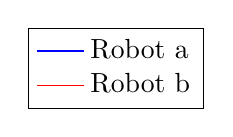
\begin{tikzpicture}

\begin{axis}[%
width=\fwidth,
height=\fheight,
scale only axis,
xmin=0,
xmax=10,
xlabel={time [$s$]},
ymin=-1,
ymax=1,
ylabel={velocity [$\frac{m}{s}$]},
legend style={draw=black,fill=white,legend cell align=left}
]
\addplot [color=blue,solid]
  table[row sep=crcr]{0	0\\
0.101010101010101	0.100838420258105\\
0.202020202020202	0.200648856522685\\
0.303030303030303	0.298413804447641\\
0.404040404040404	0.39313661214833\\
0.505050505050505	0.483851640437935\\
0.606060606060606	0.569634106908966\\
0.707070707070707	0.649609513505707\\
0.808080808080808	0.72296256147946\\
0.909090909090909	0.788945462844257\\
1.01010101010101	0.846885563602983\\
1.11111111111111	0.896192201029956\\
1.21212121212121	0.936362725104285\\
1.31313131313131	0.9669876227093\\
1.41414141414141	0.987754692360084\\
1.51515151515152	0.998452226900389\\
1.61616161616162	0.998971171723357\\
1.71717171717172	0.98930623651434\\
1.81818181818182	0.969555949182324\\
1.91919191919192	0.939921651430131\\
2.02020202020202	0.900705446202955\\
2.12121212121212	0.852307117939675\\
2.22222222222222	0.795220057023049\\
2.32323232323232	0.730026229976446\\
2.42424242424242	0.657390246682775\\
2.52525252525253	0.578052585106573\\
2.62626262626263	0.492822042588923\\
2.72727272727273	0.402567490669497\\
2.82828282828283	0.308209017490077\\
2.92929292929293	0.210708548077192\\
3.03030303030303	0.11106003812413\\
3.13131313131313	0.0102793412405343\\
3.23232323232323	-0.0906061470334077\\
3.33333333333333	-0.190567962875485\\
3.43434343434343	-0.288587058720432\\
3.53535353535354	-0.383664191806112\\
3.63636363636364	-0.474830110822239\\
3.73737373737374	-0.561155436815202\\
3.83838383838384	-0.641760137619388\\
3.93939393939394	-0.71582249922919\\
4.04040404040404	-0.782587502654202\\
4.14141414141414	-0.84137452086087\\
4.24242424242424	-0.89158425733514\\
4.34343434343434	-0.932704855531834\\
4.44444444444444	-0.964317116928778\\
4.54545454545455	-0.98609877449093\\
4.64646464646465	-0.997827777979213\\
4.74747474747475	-0.999384557612436\\
4.84848484848485	-0.990753243005677\\
4.94949494949495	-0.972021824958833\\
5.05050505050505	-0.943381258446\\
5.15151515151515	-0.905123515950137\\
5.25252525252525	-0.857638610988052\\
5.35353535353535	-0.80141062216897\\
5.45454545454545	-0.737012758318913\\
5.55555555555556	-0.665101514978822\\
5.65656565656566	-0.586409981847235\\
5.75757575757576	-0.501740369393911\\
5.85858585858586	-0.411955830830862\\
5.95959595959596	-0.317971662810619\\
6.06060606060606	-0.220745974555063\\
6.16161616161616	-0.121269920537167\\
6.26262626262626	-0.0205575962872592\\
6.36363636363636	0.0803642996702817\\
6.46464646464646	0.180466932359911\\
6.56565656565657	0.278729818677557\\
6.66666666666667	0.37415123057122\\
6.76767676767677	0.465758407025652\\
6.86868686868687	0.552617470746406\\
6.96969696969697	0.633842948448906\\
7.07070707070707	0.708606797699218\\
7.17171717171717	0.776146848283581\\
7.27272727272727	0.835774572052259\\
7.37373737373737	0.886882102029079\\
7.47474747474747	0.928948429231251\\
7.57575757575758	0.961544714026824\\
7.67676767676768	0.984338657883824\\
7.77777777777778	0.997097890943875\\
7.87878787878788	0.999692340886112\\
7.97979797979798	0.992095558932323\\
8.08080808080808	0.974384989475536\\
8.18181818181818	0.946741180583354\\
8.28282828282828	0.909445943424462\\
8.38383838383838	0.862879479381784\\
8.48484848484848	0.807516504139563\\
8.58585858585859	0.743921408256844\\
8.68686868686869	0.672742503562265\\
8.78787878787879	0.594705414024498\\
8.88888888888889	0.510605678474283\\
8.98989898989899	0.421300640588607\\
9.09090909090909	0.327700708813498\\
9.19191919191919	0.230760075325052\\
9.29292929292929	0.131466988642958\\
9.39393939393939	0.030833679061141\\
9.49494949494949	-0.0701139604006468\\
9.5959595959596	-0.170346832328096\\
9.6969696969697	-0.268843125910384\\
9.7979797979798	-0.364598733655889\\
9.8989898989899	-0.456637487633774\\
10	-0.54402111088937\\
};
\addlegendentry{Robot a};

\addplot [color=red,solid]
  table[row sep=crcr]{0	1\\
0.101010101010101	0.99490281585683\\
0.202020202020202	0.9796632259997\\
0.303030303030303	0.954436588420145\\
0.404040404040404	0.919480072752278\\
0.505050505050505	0.875150038590823\\
0.606060606060606	0.82189840263017\\
0.707070707070707	0.760268031659151\\
0.808080808080808	0.690887208377067\\
0.909090909090909	0.614463226448467\\
1.01010101010101	0.531775180091039\\
1.11111111111111	0.443666021702229\\
1.21212121212121	0.35103396849205\\
1.31313131313131	0.254823345726049\\
1.41414141414141	0.156014959925759\\
1.51515151515152	0.0556161001658067\\
1.61616161616162	-0.0453497306018852\\
1.71717171717172	-0.145853249514135\\
1.81818181818182	-0.244869886685079\\
1.91919191919192	-0.341390230048921\\
2.02020202020202	-0.434430315678286\\
2.12121212121212	-0.523041658674875\\
2.22222222222222	-0.606320922373835\\
2.32323232323232	-0.683419127290403\\
2.42424242424242	-0.753550305929445\\
2.52525252525253	-0.815999515227557\\
2.62626262626263	-0.870130124945965\\
2.72727272727273	-0.915390307713636\\
2.82828282828283	-0.951318664558728\\
2.92929292929293	-0.97754892857964\\
3.03030303030303	-0.993813698804694\\
3.13131313131313	-0.999947166176124\\
3.23232323232323	-0.995886803868673\\
3.33333333333333	-0.981674004711079\\
3.43434343434343	-0.957453659212335\\
3.53535353535354	-0.923472678494476\\
3.63636363636364	-0.880077477189673\\
3.73737373737374	-0.827710441961886\\
3.83838383838384	-0.76690542165429\\
3.93939393939394	-0.69828228503756\\
4.04040404040404	-0.62254060163933\\
4.14141414141414	-0.54045251007479\\
4.24242424242424	-0.452854846581271\\
4.34343434343434	-0.360640614001448\\
4.44444444444444	-0.264749878183483\\
4.54545454545455	-0.166160184603552\\
4.64646464646465	-0.0658765929072468\\
4.74747474747475	0.0350785690386048\\
4.84848484848485	0.135676127132719\\
4.94949494949495	0.234890552819178\\
5.05050505050505	0.331710417703216\\
5.15151515151515	0.425148704424772\\
5.25252525252525	0.514252868676963\\
5.35353535353535	0.598114549793553\\
5.45454545454545	0.67587883091213\\
5.55555555555556	0.746752954311448\\
5.65656565656566	0.810014403075603\\
5.75757575757576	0.865018266697566\\
5.85858585858586	0.911203815534403\\
5.95959595959596	0.948100217091764\\
6.06060606060606	0.975331335863734\\
6.16161616161616	0.992619567796701\\
6.26262626262626	0.999788670287321\\
6.36363636363636	0.996765558864523\\
6.46464646464646	0.983581052239521\\
6.56565656565657	0.960369558128524\\
6.66666666666667	0.927367703050975\\
6.76767676767677	0.884911920071669\\
6.86868686868687	0.833435019078179\\
6.96969696969697	0.773461774557475\\
7.07070707070707	0.705603575851525\\
7.17171717171717	0.630552194429187\\
7.27272727272727	0.54907273171308\\
7.37373737373737	0.461995819353901\\
7.47474747474747	0.37020915146548\\
7.57575757575758	0.274648435144047\\
7.67676767676768	0.176287851525489\\
7.77777777777778	0.0761301246240719\\
7.87878787878788	-0.0248037008054478\\
7.97979797979798	-0.125484668174093\\
8.08080808080808	-0.224886398621082\\
8.18181818181818	-0.321995554297938\\
8.28282828282828	-0.415822168707717\\
8.38383838383838	-0.505409738788067\\
8.48484848484848	-0.589844975855707\\
8.58585858585859	-0.668267116007629\\
8.68686868686869	-0.739876695065317\\
8.78787878787879	-0.80394369860703\\
8.88888888888889	-0.859815004003662\\
8.98989898989899	-0.906921038591359\\
9.09090909090909	-0.944781586105027\\
9.19191919191919	-0.973010682179788\\
9.29292929292929	-0.991320549013866\\
9.39393939393939	-0.99952452908148\\
9.49494949494949	-0.997538987988408\\
9.5959595959596	-0.985384167071799\\
9.6969696969697	-0.963183977052532\\
9.7979797979798	-0.931164734843692\\
9.8989898989899	-0.889652856392602\\
10	-0.839071529076452\\
};
\addlegendentry{Robot b};

\end{axis}
\end{tikzpicture}%
  \caption{Example figure created with \texttt{matlab2tikz}.}
  \label{fig:example_tikz_figure}
\end{figure}

An alternative which you might want to consider is \texttt{matlabfrag} and \texttt{mlf2pdf}.
Especially when there are many data points in your figure you might run into problems when using tikz.
Again, you can find a short example on how to use \texttt{mlf2pdf} in the \texttt{create\_figures.m} scriptin in the \texttt{matlab\_figures} folder.
This script makes use of the two functions \texttt{matlabfrag.m} and \texttt{mlf2pdf.m} to create a PDF which you can then include into matlab.
These two files can be downloaded \href{http://www.mathworks.ch/matlabcentral/fileexchange/28545-matlabfrag-to-pdf}{here} and \href{http://www.mathworks.ch/matlabcentral/fileexchange/21286-matlabfrag}{here}.

\begin{figure}[H]
     \centering
     \includegraphics[width=0.85\textwidth]{matlab_figures/example_matlabfrag_figure.pdf}
     \caption{Example figure created with \texttt{mlf2pdf}.}
     \label{fig:example_matlab_fig}
  \end{figure}


\section{Including Code in your Document}

You may include samples from your Matlab code using the \texttt{lstlistings} environment, for example:

  \lstset{language=Matlab,numbers=none}
  \begin{lstlisting}[frame=lines, caption=Matlab Example, label=matlabexample]
  % Evaluate y = 2x
  for i = 1:length(x)

    y(i) = 2*x(i);

  end
  \end{lstlisting}

  \lstset{language=C++,numbers=none,caption=C++ Example, label=cppexample}
  \begin{lstlisting}[frame=lines]
  // sum all elements in a list
  int sum=0;
  for(list<int>::iterator it=mylist.begin(); it!=mylist.end(); ++it)
    sum += *it;
  \end{lstlisting}

%\chapter{RPG Notation Style}\label{chap:notation}

This chapter presents some conventions on notation that we use at the Robotics and Perception Group.
Try to stick to those conventions since a unique style makes it easier to review the report.

\section{Variable styles in \LaTeX}

Use lowercase and bold letters for vectors, e.g. $\textbf{x}$, uppercase and bold letters for matrices, e.g. $\textbf{R}$, and lowercase letters with normal weight for scalars, e.g. $s$.

\section{Coordinate Systems and Rotations}

We use the notation introduced by Prof. Glocker in the course ``Mechanik 3'' at ETHZ to express coordinate frames, rotations and vectors.
Refer to Chapter~5 ``Kinematik'' in the lecture script for more details \footnote{\url{http://mitschriften.amiv.ethz.ch/main.php?page=3&scrid=1&pid=87&eid=1}}.
Figure \ref{fig:notation} gives an overview of how coordinate transformations and vectors are specified.
Observe that the coordinate system in which a vector is expressed is always written as index before the variable, e.g. $_B\mathbf{t}_{AB}$ is the vector from $A$ to $B$ expressed the coordinate system $B$.
For the ease of reading, the index for the origin coordinate frame can be omitted: $_O\mathbf{t}_k := \mathbf{t}_k$.

\begin{figure}[H]
     \centering
     \includegraphics[scale=0.8]{img/notation}
     \caption{Notation overview.}
     \label{fig:notation}
\end{figure}
  
$A$ and $B$ are two adjacent coordinate frames and $O$ is the frame of origin.
$\mathbf{R}_{AB}$ describes the coordinate transformation from frame $B$ to frame $A$, thus it holds that 
	\[
		\begin{aligned}
			_O\mathbf{t}_k  &= \mathbf{R}_{OB} \ _B\mathbf{f}_k, \\
			\mathbf{R}_{OB} &= \mathbf{R}_{OA} \ \mathbf{R}_{AB}.
	  \end{aligned} 
	\]

\section{Measured, estimated and target values}

For controllers and estimators please specify the variables as follows in the report:

	\[
		\begin{aligned}
			\text{true value:} \quad & \mathbf{x} \\
			\text{estimated value:} \quad & \hat{\mathbf{x}} \\
			\text{measured value:} \quad & \tilde{\mathbf{x}} \\
			\text{desired value:} \quad & \mathbf{x}_\text{des} \\
      \text{error value:} \quad & \mathbf{x}_\text{e} \\
      \text{equilibrium value:} \quad & \mathbf{x}^* \\
		\end{aligned}
	\]

\chapter{Discussion}\label{chap:discussion}

TODO
Explain both the advantages and limitations of your approach.

\section{Conclusion}\label{sec:conclusion}
In this thesis we presented a complete framework to permits a quadrotor to find, approach and land on a moving platform. We explained all the modules that make up the system, showing in detail the computation we perform in order to complete the assigned task. \\
Several experiments were carried in simulation and in the real world to demonstrate the functionality of our system. From these experiments we demonstrate robustness of the framework up to a certain velocity, after which the trajectory generation and the self state estimation modules start to fail.\\

\section{Future Work}\label{sec:future_work}
There are several upgrades that can be done to this frameworks. The major problems are related to the not always robust state estimation and the issues with the trajectory generator ( described in \ref{sec:trajectory_problem}).\\
 Following we describe what solution can be applied in future to solve these problems.

\subsection{State estimation using also GPS and Teraranger}
A future upgrade that we should do is to fuse multiple sensor to have a more robust and precise state estimation.\\
As a matter of fact MSF can combine easily different sources of data, filtering them with the IMU information.
The main two sensor we can add for this upgrade can be:
\begin{itemize}
\item GPS: it gives a 3D absolute position with not a high accuracy, but are always available in outside environment, and can be useful to have a continue state estimation used to initialized (and reinitialized if it fails) the visual odometry. Of course the uncertainty related to this measure will be much more higher w.r.t the one from SVO, but it is MSF's duty taking in account these information and filtering the data in the right way.
\item Teraranger \cite{teraranger}: it is distance sensor for robotics, it can operate both in inside and outside environment, it is very light and can be really useful to have an estimation of the height of the quadrotor. It is in fact well known that both VO and GPS systems have much more error in the depth component, so the data from this sensor can be correct all the wrong estimations from the other two sources. 
\end{itemize}

\subsection{Change the controller}
As describe before the trajectory generator has some issues that must be resolved \label{sec:trajectory_problem}}. The approach to solve these problems can be:
\begin{itemize}
\item make the flight controller more sensitive: right now the replanning does not work because the first desired state of the trajectory is too close to the current state to generate a correct control action. Making the controller more response at little variation can solve this problem.\\
A method to increase the sensitivity is tuning the controller gains, but this can lead to a unstable behavior, so further studies must be done.
\item change both the trajectory and the contorller: implementing a new contorller like a LQR controller \cite{wiki_lqr} that takes in account both the dynamic of the quad and the platform and directly calculate the control actions necessary to arrive at a certain final state.\\  In this case the state machine should not predict in advance where the platform will be in $T$ seconds because this prediction is directly done by the LQR controller. The main problem with this type of controller is tuning the weights in the cost function to have a nice and smooth flight. \\ 
Furthermore we can implement a continuous replanning of the control actions of the LQR, leading with an MPC framework. This solution, as described in the introduction of the thesis, is really computational expensive and before implementing it, we must understand if it can run onboard on our quadrotor.
\end{itemize} 

\subsection{Cross detector}
In the final challenge the moving platform will be signed with the marker in figure \ref{fig:finalplatform}. \\
In order to have a measurement update in the low-altitude EKF we have to implement a cross detector: instead of estimating the 4dof pose of the platform from the AR-tag detection, we must be able to extract the same information from the cross mark.\\

The detector itself should not be really hard to implement  (it consists in a new Pnp problem) the only problem can be due to the symmetry of the cross that does not allow to detect a unique solution for the yaw orientation. On the other end once we are estimating the initial yaw angle we are able to detect correctly the changing in orientation, as far as between two consecutive measures the platform rotates a few degrees: we cannot distinguish between rotations of $k90^o$, but we know that two measures close in time has also close degree because the angular velocity of the platform is not really high.\\

From the point of view of our framework we can simply substitute the detection module and everything still working: this new detector should provide the same data of the AR-tag detector used in this thesis, and so it can directly be used as update step on the EKF already implemented.\\

\cleardoublepage

% Appendix______________________________________________________________________
\appendix
%\input{chapters/10_appendix}

% Bibliography__________________________________________________________________

\bibliographystyle{unsrt}
\bibliography{bibtex/references.bib}

\end{document}
